% Chapter Template

\chapter{Results}
\label{chap:4:results}

\label{sec:results:clinical}

In this chapter, I first discuss the textual characteristics of both samples and verbosity patterns (\ref{sec:results:clinical:sample_length}), then turn to the interaction between the social variables and the target variables, as well as the relation between the target variables and the text length (\ref{sec:results:clinical:control_variables}). Afterwards, each group of metrics is discussed separately for both languages (\ref{sec:results:clinical:lexical}-\ref{sec:results:clinical:LM}). Finally, I present a cross-group (\ref{sec:results:clinical:cross_group}) and a cross-linguistic (\ref{sec:results:clinical:cross_linguistic}) comparison of the studied metrics.

%-----------------------------------
%	section 1
%-----------------------------------
\section{Textual Characteristics of the Samples}
\label{sec:results:clinical:sample_length}

As NAP patients are believed to be less verbose, it is important to take the differences in text length into account. Table \ref{tab:data:length} summarizes the length characteristics of both German and Russian samples. Unlike what has been reported previously, the overall text length, i.e. word count, seems to be explained more by the number of sentences than by their length, though sentence length also plays some role, especially in the German sample. It also seems to play some role in the overall verbosity on two of the tasks in the Russian sample, adventure and chair, - the shortest and the longest one, respectively. 

Figures \ref{fig:data:de:length} and \ref{fig:data:ru:length} show the relation between the word count and both sentence count and mean sentence length, as well as the correlation coefficient, underlining the differences in the components contributing to the text length across the tasks and languages. These differences imply that the mean sentence length would serve as a strong baseline for performance only on some tasks, while on others only the number of sentences, and, possibly, the word count, would function as such. For the tasks, where the differences in mean sentence length are prominent, it is especially important to account for the intrinsic relation between some of the metrics and mean sentence length. However, no such correction is required for the number of sentences, as there seems no intrinsic relation between the number of sentences and the metric values for any of the metrics used, except the verbosity\footnote{It is possible that the moving window procedure does not entirely remove the effects of verbosity from the graph-based metrics. These effects may come via the number of sentences, rather than sentence length, though with the latter the graph-based metrics are indeed not intrinsically related. Yet, we do not explore this question further in the present work.}.

\begin{table}[h]
\resizebox{\textwidth}{!}{%
\begin{tabular}{llllll}
\hline
\textbf{} & \textbf{German} & \textbf{Russian} & \textbf{} & \textbf{} & \textbf{} \\
\textbf{task} & \textbf{} & \textbf{adventure} & \textbf{chair} & \textbf{present} & \textbf{sportsman} \\ \hline
n words           & \begin{tabular}[c]{@{}l@{}}184.2\\ (117.4)\end{tabular} & \begin{tabular}[c]{@{}l@{}}129.8 \\ (82.1)\end{tabular} & \begin{tabular}[c]{@{}l@{}}168.4 \\ (120.9)\end{tabular} & \begin{tabular}[c]{@{}l@{}}140.8 \\ (107.7)\end{tabular} & \begin{tabular}[c]{@{}l@{}}134.4 \\ (86.0)\end{tabular} \\
n sents & 17.9 (9.3) & 18.7 (11.0) & 20.4 (15.0) & 15.1 (12.7) & 17.7 (10.1) \\
mean sent len & 10.0 (2.8) & 6.9 (1.5) & 8.1 (1.6) & 9.9 (4.7) & 7.8 (2.2) \\
r n sents & 0.88 & 0.93 & 0.95 & 0.95 & 0.93 \\
r n mean sent len & 0.59 & 0.36 & 0.38 & 0.08 & 0.11 \\ \hline
\end{tabular}
}
\captionsetup{width=\textwidth}
\caption[Text Length Characteristics]{\label{tab:data:length} Statistics of the mean length of each task between the languages. Standard deviation is provided in parenthesis for each mean value. \\ `n words' stands for the word count, `n sents' for sentence count, and `mean sent len' for mean sentence length. `r n sents' indicates the correlation coefficient of the word count with the sentence count and `r mean sent length' that of the word count with mean sentence length.}
\end{table}

\begin{figure}[ht!]
\begin{center}
    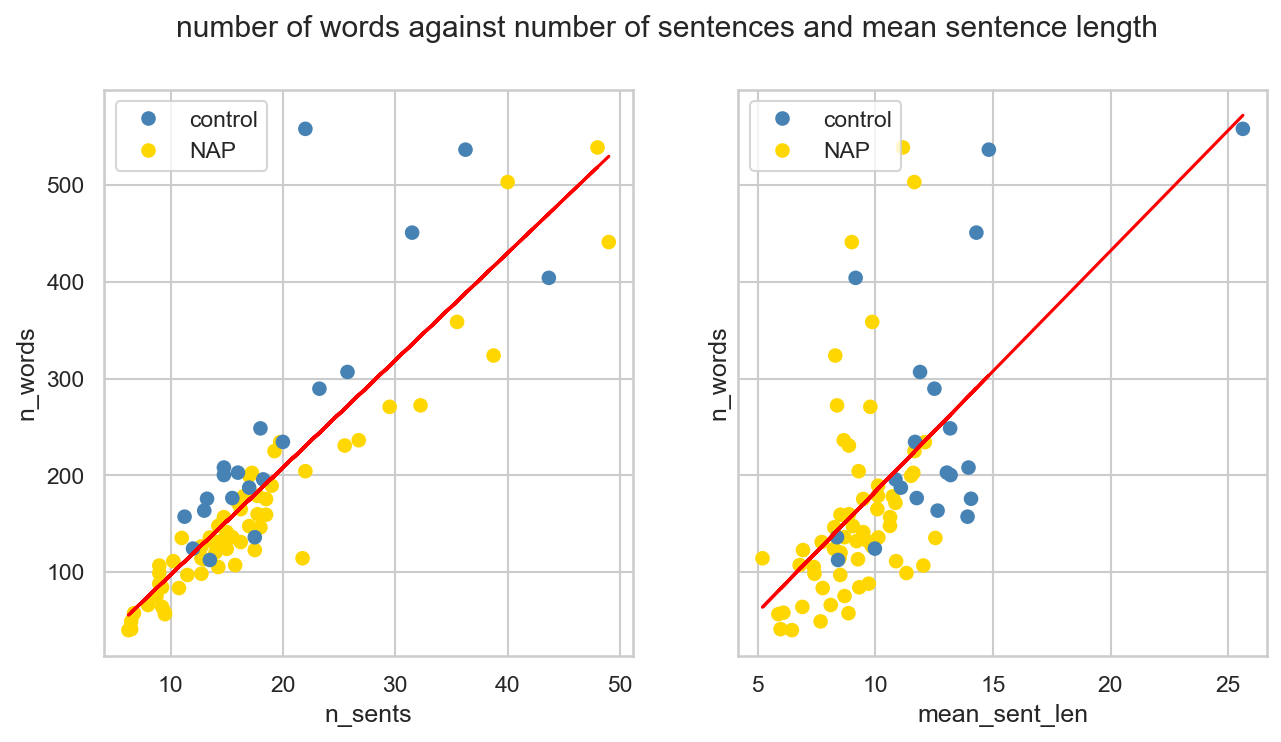
\includegraphics[width=0.7\textwidth]{Figures/chapter_4/de_n_words_n_sents.png} 
\caption[German Clinical Dataset: Length Characteristics]{\label{fig:data:de:length} The correlation between word count and both sentence count and mean sentence length on the German sample, with colors indicating controls and NAP groups.}
\end{center}
\end{figure}

\begin{figure}[p]
\begin{center}
    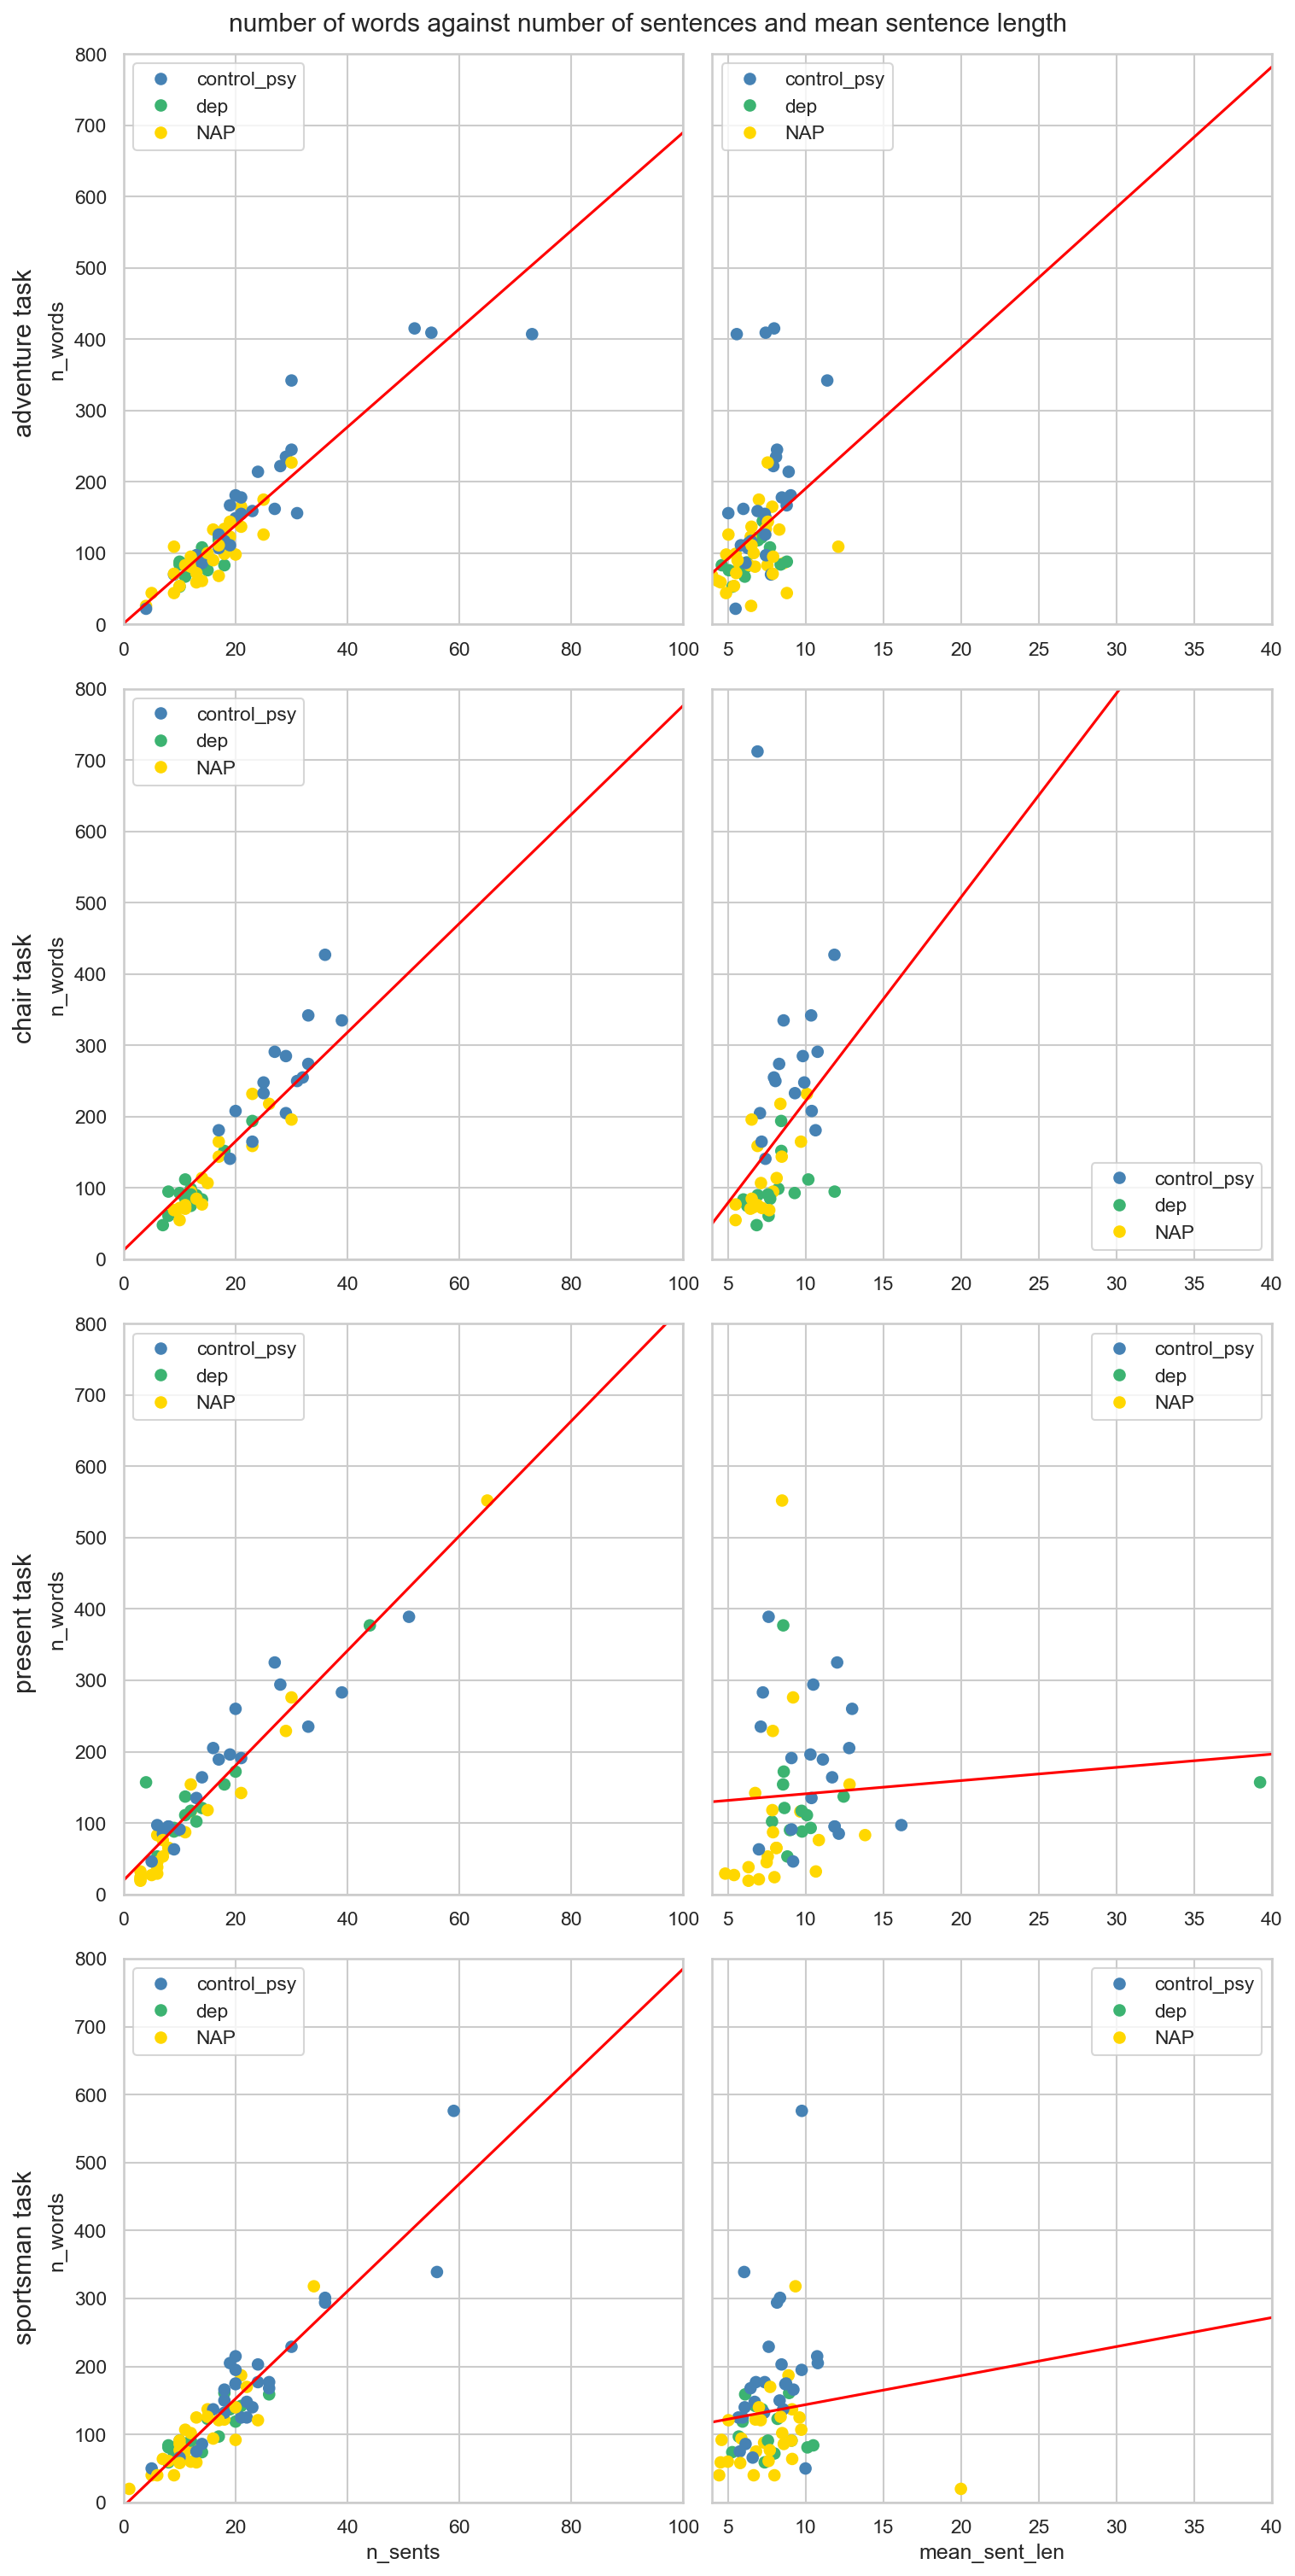
\includegraphics[width=0.7\textwidth]{Figures/chapter_4/ru_n_words_n_sents.png} 
\caption[Russian Clinical Dataset: Length Characteristics]{\label{fig:data:ru:length} The correlation between word count and both sentence count and mean sentence length on the Russian sample for each of the tasks, with colors indicating controls, depression and NAP groups.}
\end{center}
\end{figure}

\pagebreak



%-----------------------------------
%	section 2
%-----------------------------------
\section{Control Variables}
\label{sec:results:clinical:control_variables}

\subsection{German}

After correcting for multiple testing, there remained a significant negative correlation of symptom severity with mean sentence length for negative symptom scales: SANS and PANSS negative (r \textless -0.4, p before correction \textless 0.001). There was no relation between sentence length and sex, age, years of education, or verbal IQ. 

As for the relation between the control variables and the tested metrics, there was no difference in metric between the sexes, and no significant correlation with age, years of education, or verbal IQ, after Bonferroni correction.

\subsection{Russian}

After correcting for multiple testing, there was no significant correlation with mean sentence length for any of the psychiatric scales or social variables, though this may be both because of a high number of comparisons and a lower importance of mean sentence length for overall word count in the Russian sample. 

There also was no correlation between the metrics and the control variables, after controlling for multiple comparisons, with no significant correlation with age or ears of education, and no effect of sex, though here as well it may be due to a high number of comparisons.


%-----------------------------------
%	section 3
%-----------------------------------
\section{Scale and Task Effects}

Table \ref{tab:results:scales_tasks} summarizes the performance of the tested metrics across tasks and scales, showing the number of metrics correlated with each psychiatric scale, as well as the number of metrics among them which were also uncorrelated with mean sentence length.

\begin{table}[ht]
\resizebox{\textwidth}{!}{%
\begin{tabular}{lllllll}
\hline
    & \textbf{German}     & \textbf{Russian}   &        &         &           &         \\
    & \textbf{total (De)} & \textbf{adventure} & \textbf{chair}  & \textbf{present} & \textbf{sportsman} & \textbf{total (Ru)} \\ 
\hline
\textbf{PANSS total}  & 16 (3)    & 9 (2)     & 12 (5) & 18 (13) & 8 (7)     & 30 (17) \\
\textbf{PANSS\_pos}   &  1 (0)    & 1 (1)     & 12 (5) & 13 (11) & 10 (8)    & 24 (15) \\
\textbf{PANSS\_neg}  & 12 (3)      & 8 (1)     & 5 (3)  & 17 (12) & 8 (7)     & 28 (15) \\
\textbf{PANSS\_o}    & 14 (2)      & 7 (2)     & 11 (4) & 18 (13) & 7 (6)     & 28 (16) \\
\textbf{SANS}        & 10 (3)      & -         & -      & -       & -         & -       \\
\textbf{SAPS}         & 5 (1)     & -         & -      & -       & -         & -       \\
\textbf{dep severity} & -         & 0 (0)     & 9 (2)  & 0 (0)   & 0 (0)     & 9 (2)   \\
\textbf{td severity}  & -         & 0 (0)     & 3 (2)  & 13 (11) & 4 (3)     & 19 (15) \\ 
\hline
\textbf{total }       & 21 (4)    & 10 (2)     & 17 (5) & 23 (18) & 10 (8)    & 30 (20)    \\ 
\hline
\end{tabular}
}
\captionsetup{width=\textwidth}
\caption[Scale and Task Effects]{\label{tab:results:scales_tasks} The number of metrics correlating above 0.3 with the target scale (or having pseudo r squared above 0.9) and either do not correlate with mean sentence length above the threshold of 0.3 or outperform this baseline metric. In parenthesis are the numbers of metrics not correlating with sentence length above 0.3.}
\end{table}

\subsection{German}
The overall differences between the scales are summarized in table \ref{tab:results:scales_tasks}. On the German sample, negative symptoms predominate, and, therefore, across the tested metrics, the correlation with the negative symptoms is stronger than with the positive. Additionally, SAPS, which is dedicated solely to the positive symptoms, was more detailed than the corresponding PANSS subscale. Thus, the correlation with SAPS across the metrics was stronger than with the positive PANSS subscale. Yet, SANS and PANSS negative subscale were close to each other. The total PANSS score, as it encompasses both positive and negative symptoms, was correlated with most metrics. On the German sample, the correlation with mean sentence length was frequent for the well-performing metrics, yet many metrics outperformed this baseline. As for the group differences in the metrics on the German sample, they are discussed below for each metric type. 

\subsection{Russian}
The same table (\ref{tab:results:scales_tasks}) shows the overall effects of both tasks and scales for the Russian sample. On it, negative symptoms also predominate, and across all PANSS subscales, the symptoms are more severe than in the German sample. Thus, both positive and negative, as well as general symptoms correlated with some of the metrics. Like on the German sample, PANSS total score correlated with most metrics, however, all PANSS subscales followed closely, the positive symptoms being hardest to predict. TD severity was slightly more less predictable, being easiest to predict on one of the tasks (present), and depression severity could only be predicted on one task (chair). No metric was sensitive enough to reliably differentiate between the groups on the Russian sample, as all bootstrap quantile-based error bars crossed zero for all tasks and metrics\footnote{Due to this absence of any meaningful difference between the groups, the t-test results for the Russian sample are not discussed in any more detail in the present work.}.

The symptom severity was most strongly correlated with the metrics calculated on present task, followed by chair task, sportsman task, and adventure task. This means that the two picture-elicited tasks, sportsman and adventure, were the hardest to predict the symptom severity on. 

As verbosity was more explained by mean sentence length for chair and adventure tasks, these two showed the most difference between the metrics that did not correlate with sentence length and those that did but outperformed it. On the other two tasks, the sentence length did not serve as a strong baseline and the aforementioned difference was therefore not as pronounced.


%-----------------------------------
%	section 4
%-----------------------------------
\section{Lexical Methods}
\label{sec:results:clinical:lexical}
This section covers the performance of the selected lexical metrics, namely, lemma-token ratio (LTR), moving average lemma-token ratio (MALTR), and word count (n words) across target variables in both languages.

\subsection{German}
Figure \ref{fig:results:lexical:de} shows the performance of each lexical metric on SANS, SAPS, and PANSS subscales. On the German sample, LTR positively correlated with the negative symptom scales (PANSS negative and SANS), total PANSS, and PANSS general subscale. MALTR, on the other hand, weakly negatively correlated with both SANS and SAPS. Finally, word count negatively correlated with the negative symptom scales.

\begin{figure}[h!]
    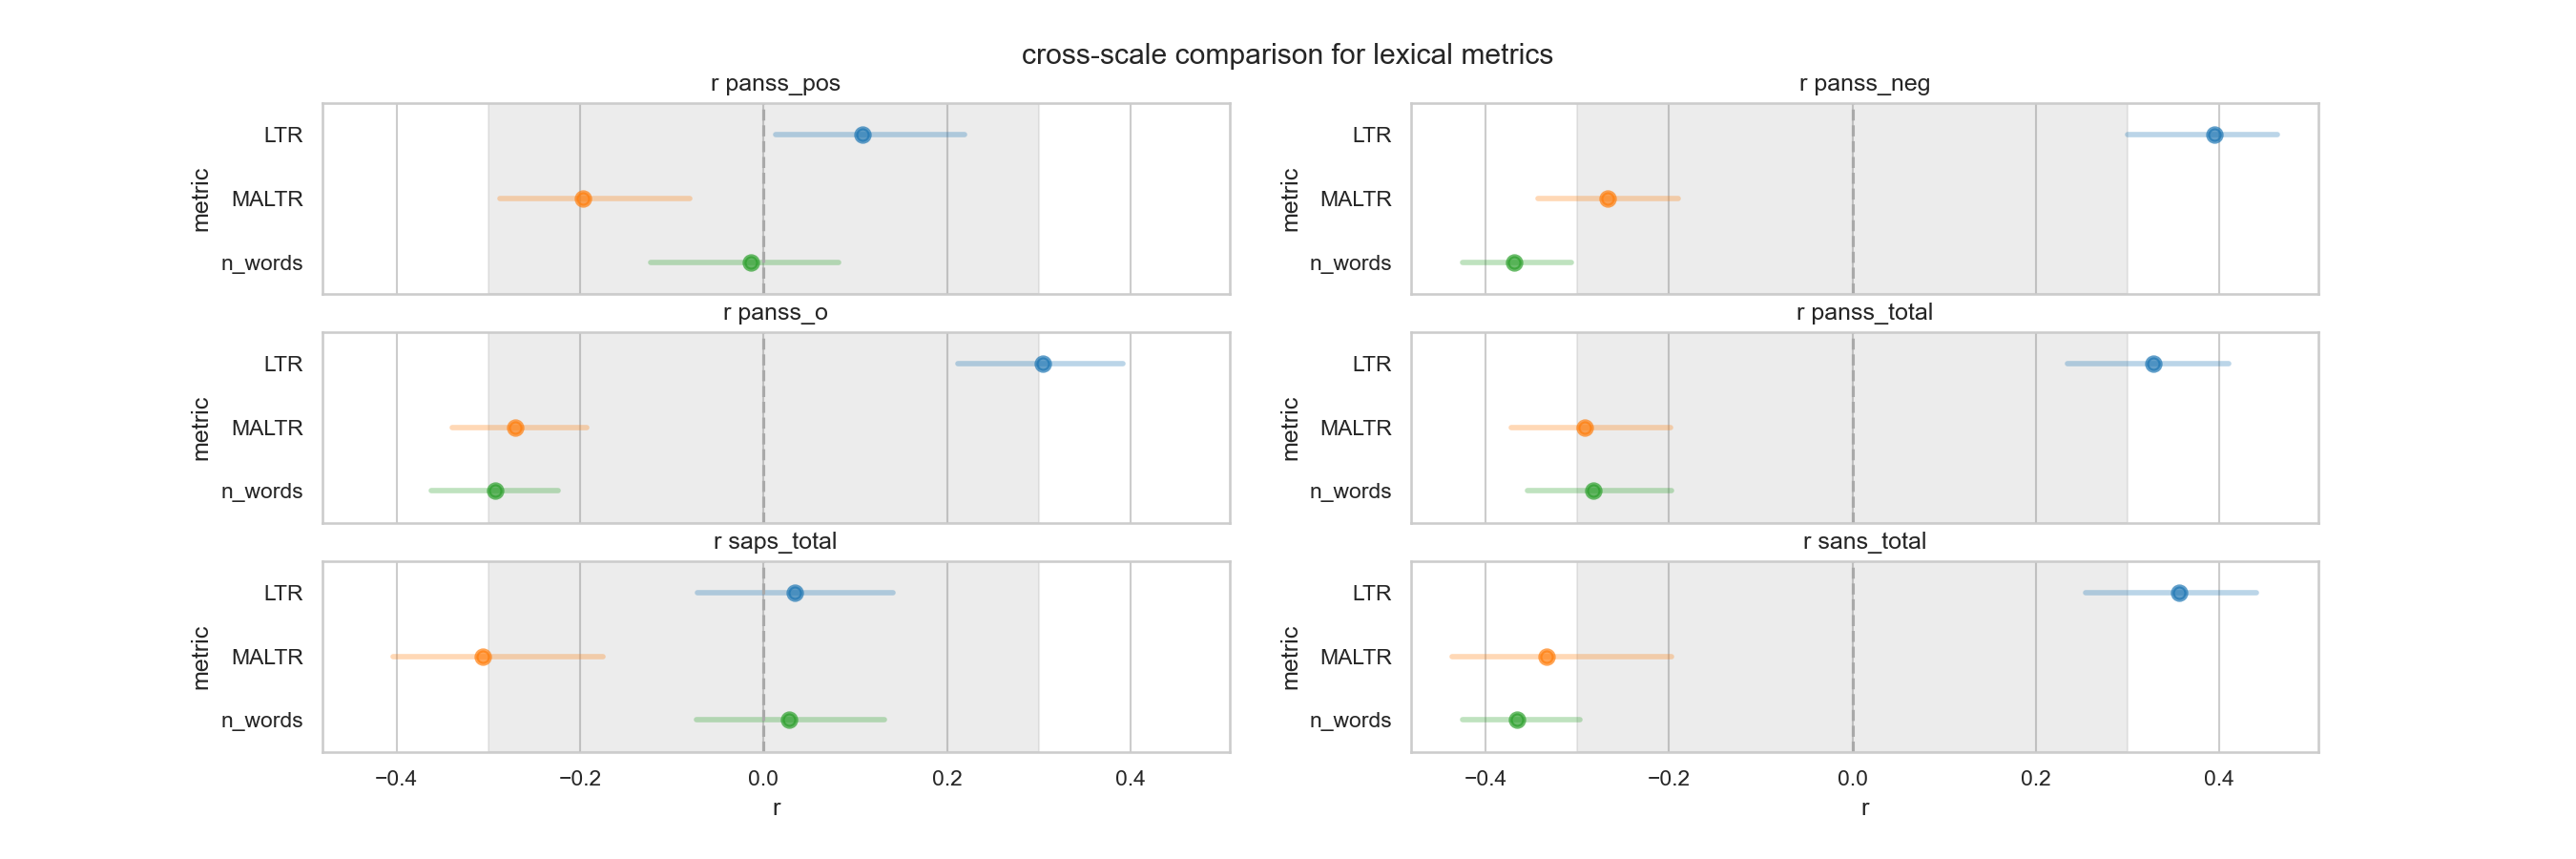
\includegraphics[width=1.2\textwidth, center]{Figures/chapter_4/lexical/de_scale_r.png} 
\captionsetup{width=\textwidth}
\caption[Lexical Metrics: German]{\label{fig:results:lexical:de} Pearson's r correlation coefficient with each scale for the lexical metrics on the German dataset. Grey indicates the values below the 0.3 threshold in absolute value.}
\end{figure}

As shown in figure \ref{fig:results:lexical:de:ttest}, the correlation with mean sentence length closely matched the performance of each metric on the t-test. The LTR was higher in the patient group, while the word count was lower, with no difference in MALTR. All three metrics correlated with mean sentence length, LTR negatively, and MALTR and word count positively.

\begin{figure}[ht!]
    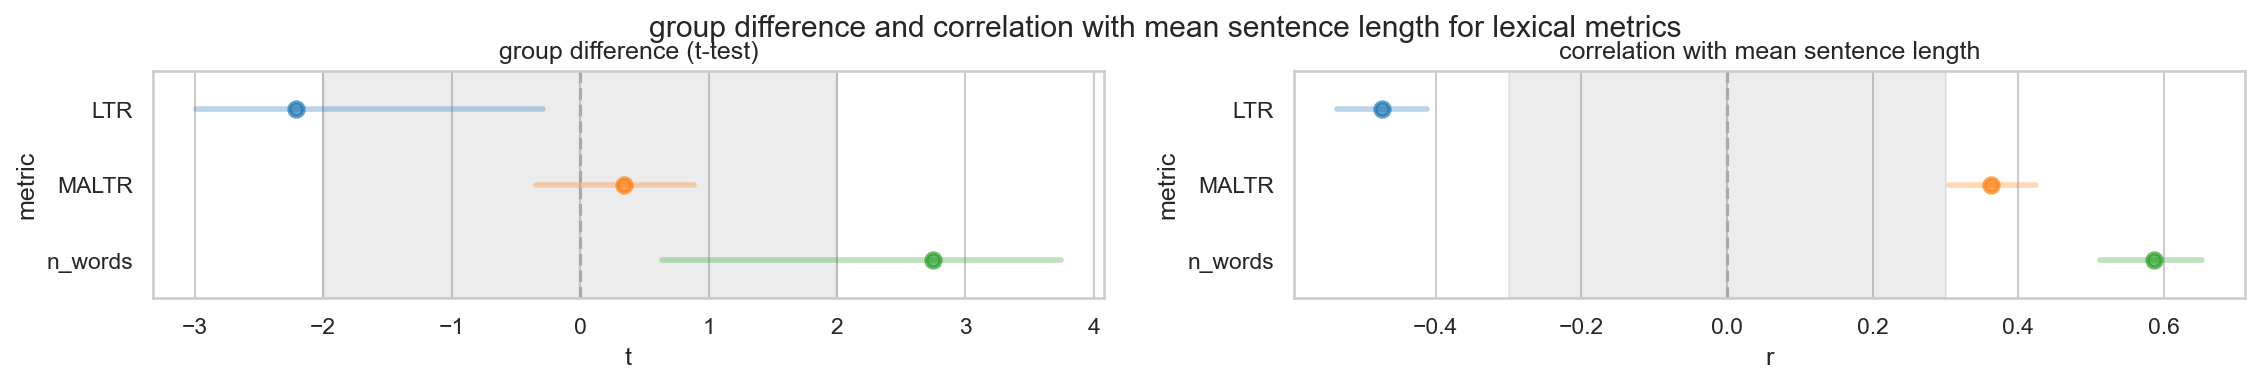
\includegraphics[width=\textwidth, center]{Figures/chapter_4/lexical/de_t_test_corr_len.png} 
\captionsetup{width=\textwidth}
\caption[Lexical Metrics: German (T-Test)]{\label{fig:results:lexical:de:ttest} T-test and Pearson's r correlation coefficient with mean sentence length for the lexical metrics on the German dataset. Grey indicates the values below 2 for the t score and below the 0.3 threshold in absolute value for the correlation coefficient.}
\end{figure}


\subsection{Russian}
On adventure task, shown in figure \ref{fig:results:lexical:ru:ad}, LTR did not perform on any of the scales. MALTR correlated negatively with PANSS negative and general scales, as well as the total PANSS score. Word count correlated negatively with all PANSS scales. None of the metrics could detect TD or depression severity.

\begin{figure}[ht!]
    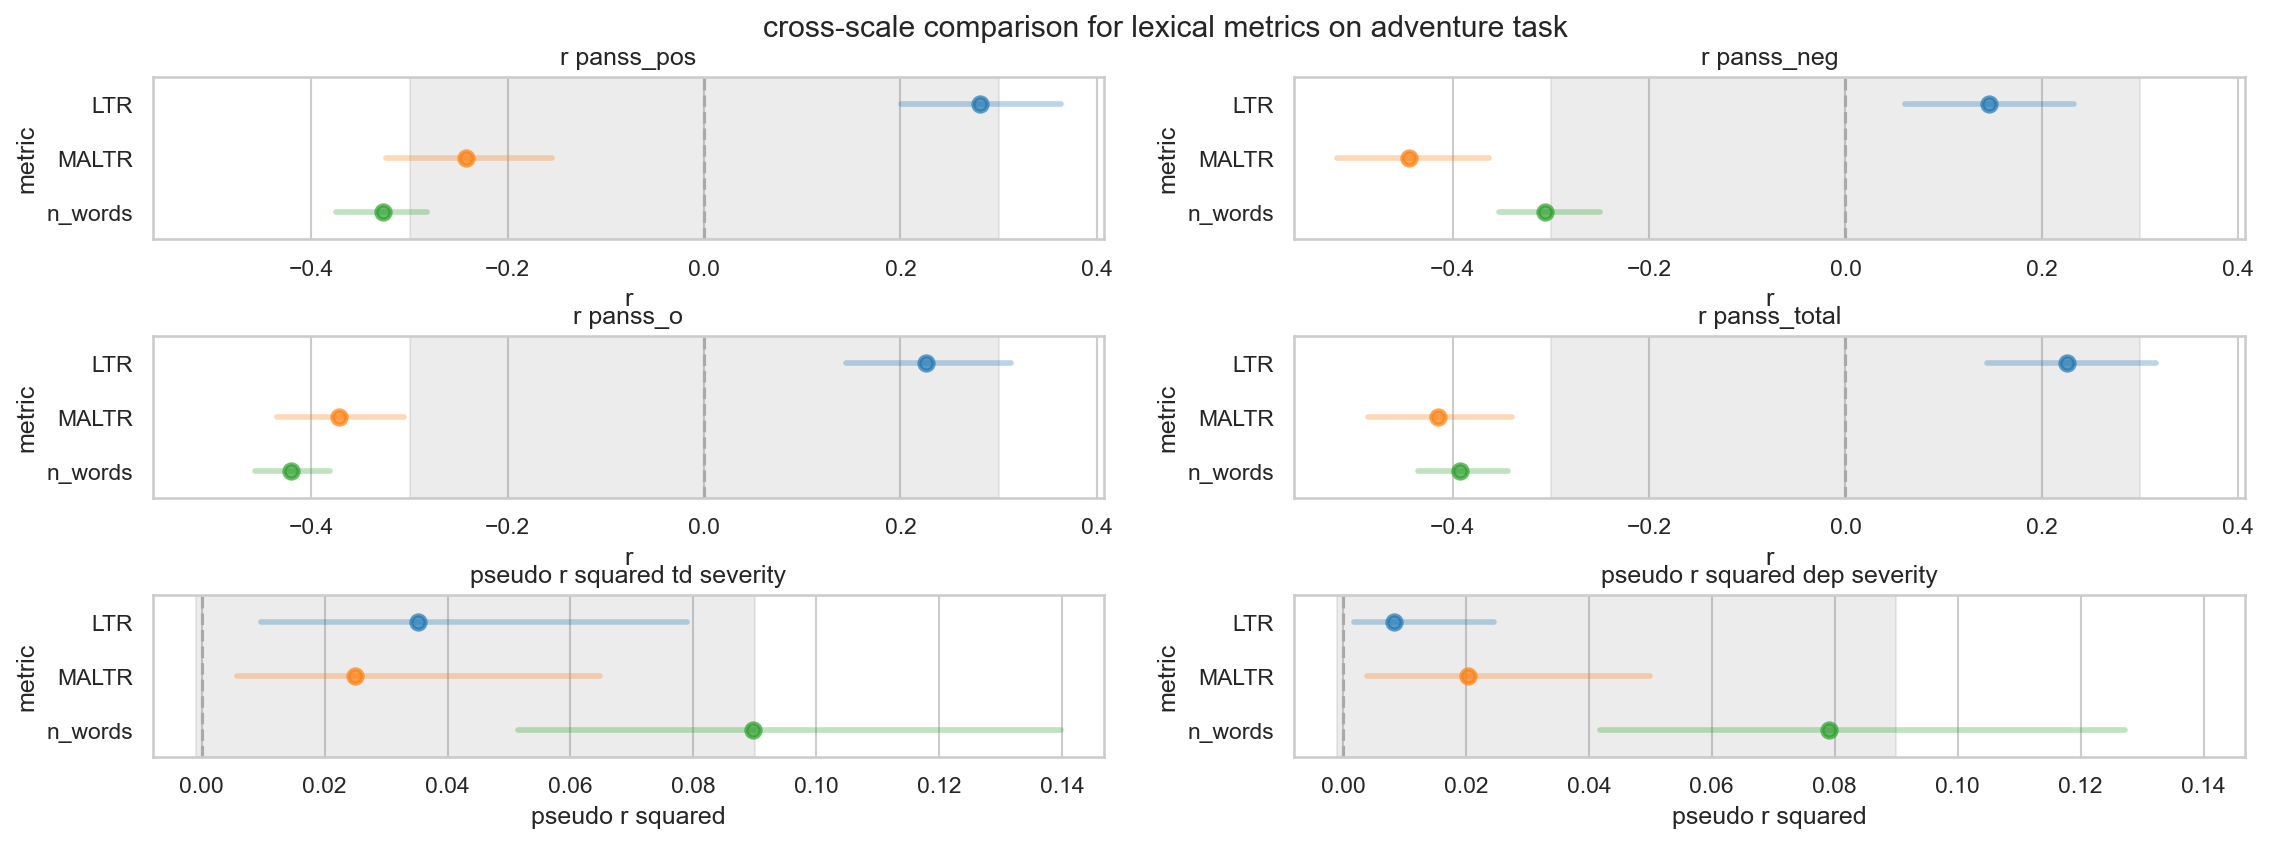
\includegraphics[width=0.9\textwidth, center]{Figures/chapter_4/lexical/ru_adventure_scale_r.png} 
\captionsetup{width=\textwidth}
\caption[Lexical Metrics: Russian, Adventure Task]{\label{fig:results:lexical:ru:ad} Pearson's r correlation coefficient and pseudo r squared for each scale for the lexical metrics on the Russian dataset, adventure task. Grey indicates the values below the 0.3 threshold in absolute value or pseudo r squared below 0.09.}
\end{figure}

On chair task, shown in figure \ref{fig:results:lexical:ch}, LTR correlated positively with all PANSS subscales, and was also predictive of depression severity. Conversely, MALTR and word count both correlated negatively with all PANSS subscales, and word count was also predictive of depression severity on chair task.

\begin{figure}[ht!]
    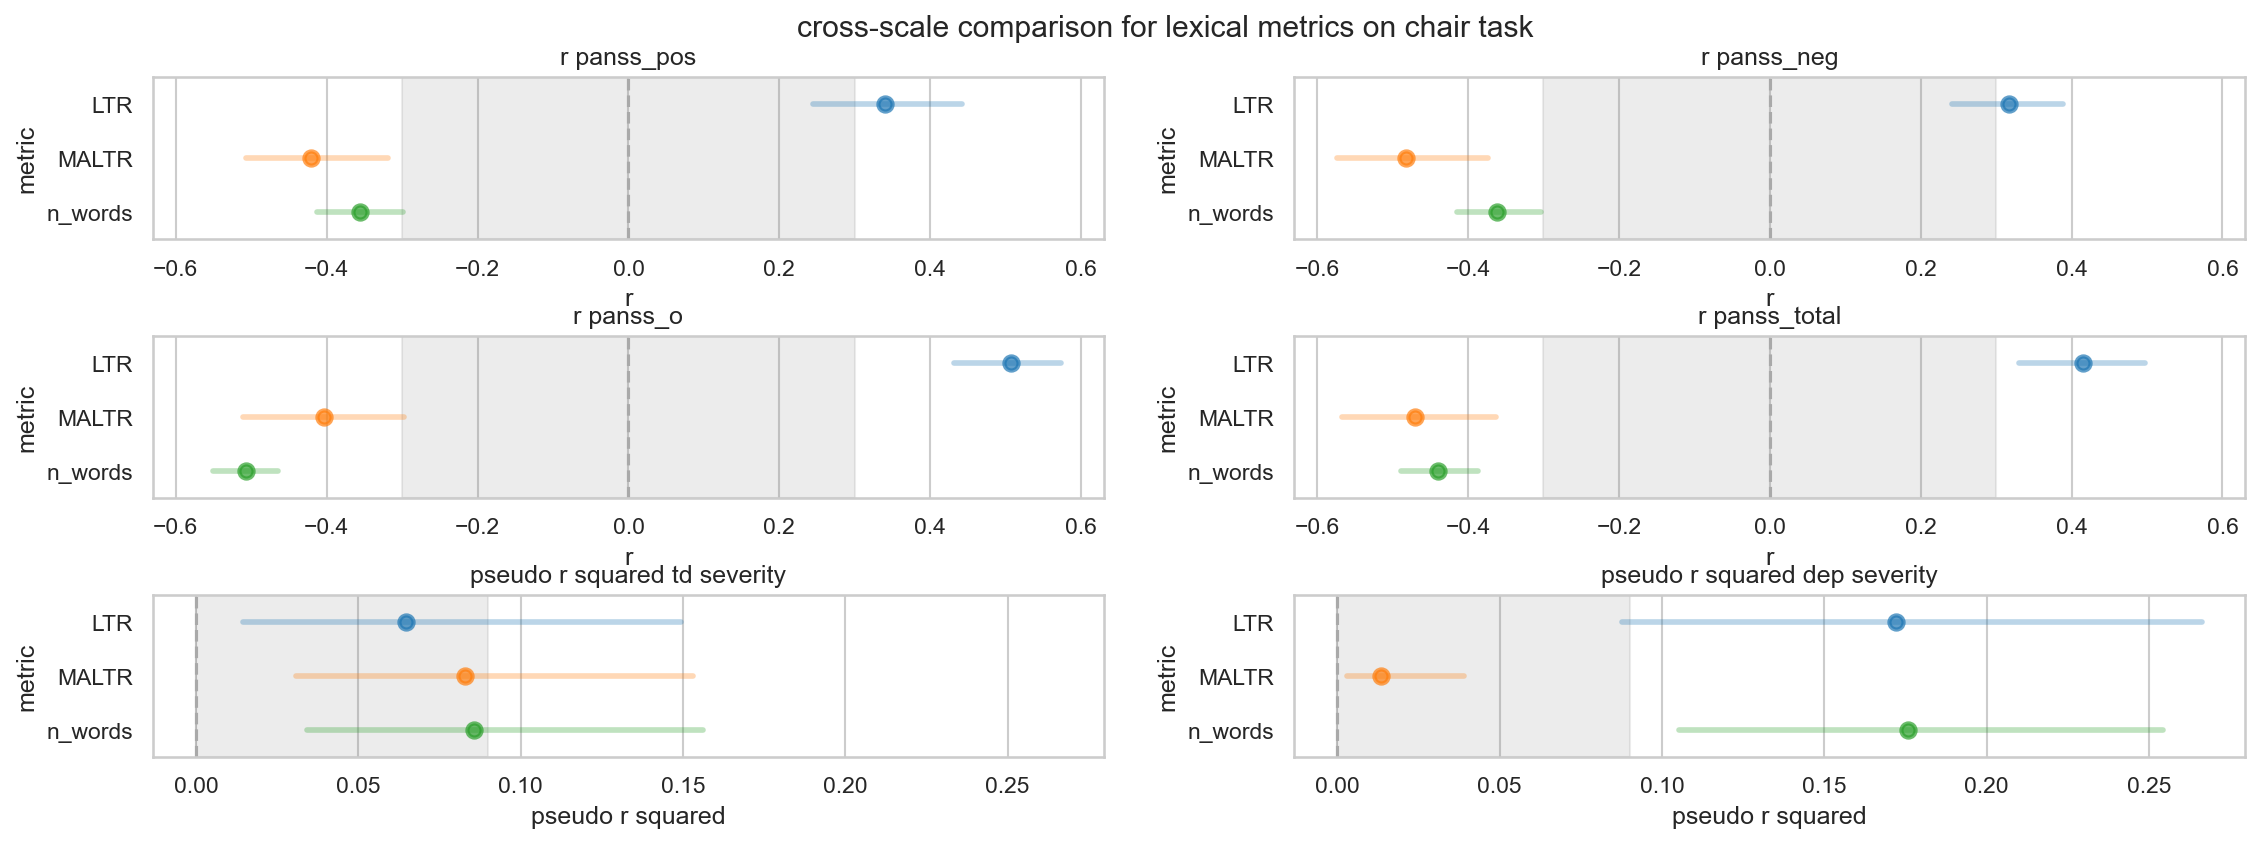
\includegraphics[width=0.9\textwidth, center]{Figures/chapter_4/lexical/ru_chair_scale_r.png} 
\captionsetup{width=\textwidth}
\caption[Lexical Metrics: Russian, Chair Task]{\label{fig:results:lexical:ch} Pearson's r correlation coefficient and pseudo r squared for each scale for the lexical metrics on the Russian dataset, chair task. Grey indicates the values below the 0.3 threshold in absolute value or pseudo r squared below 0.09.}
\end{figure}

On present task, shown in figure \ref{fig:results:lexical:ru:pr}, LTR correlated positively with all PANSS subscales and was predictive of TD severity. MALTR correlated with PANSS negative only, and word count correlated negatively with all PANSS subscales and was also predictive of TD severity.

\begin{figure}[ht!]
    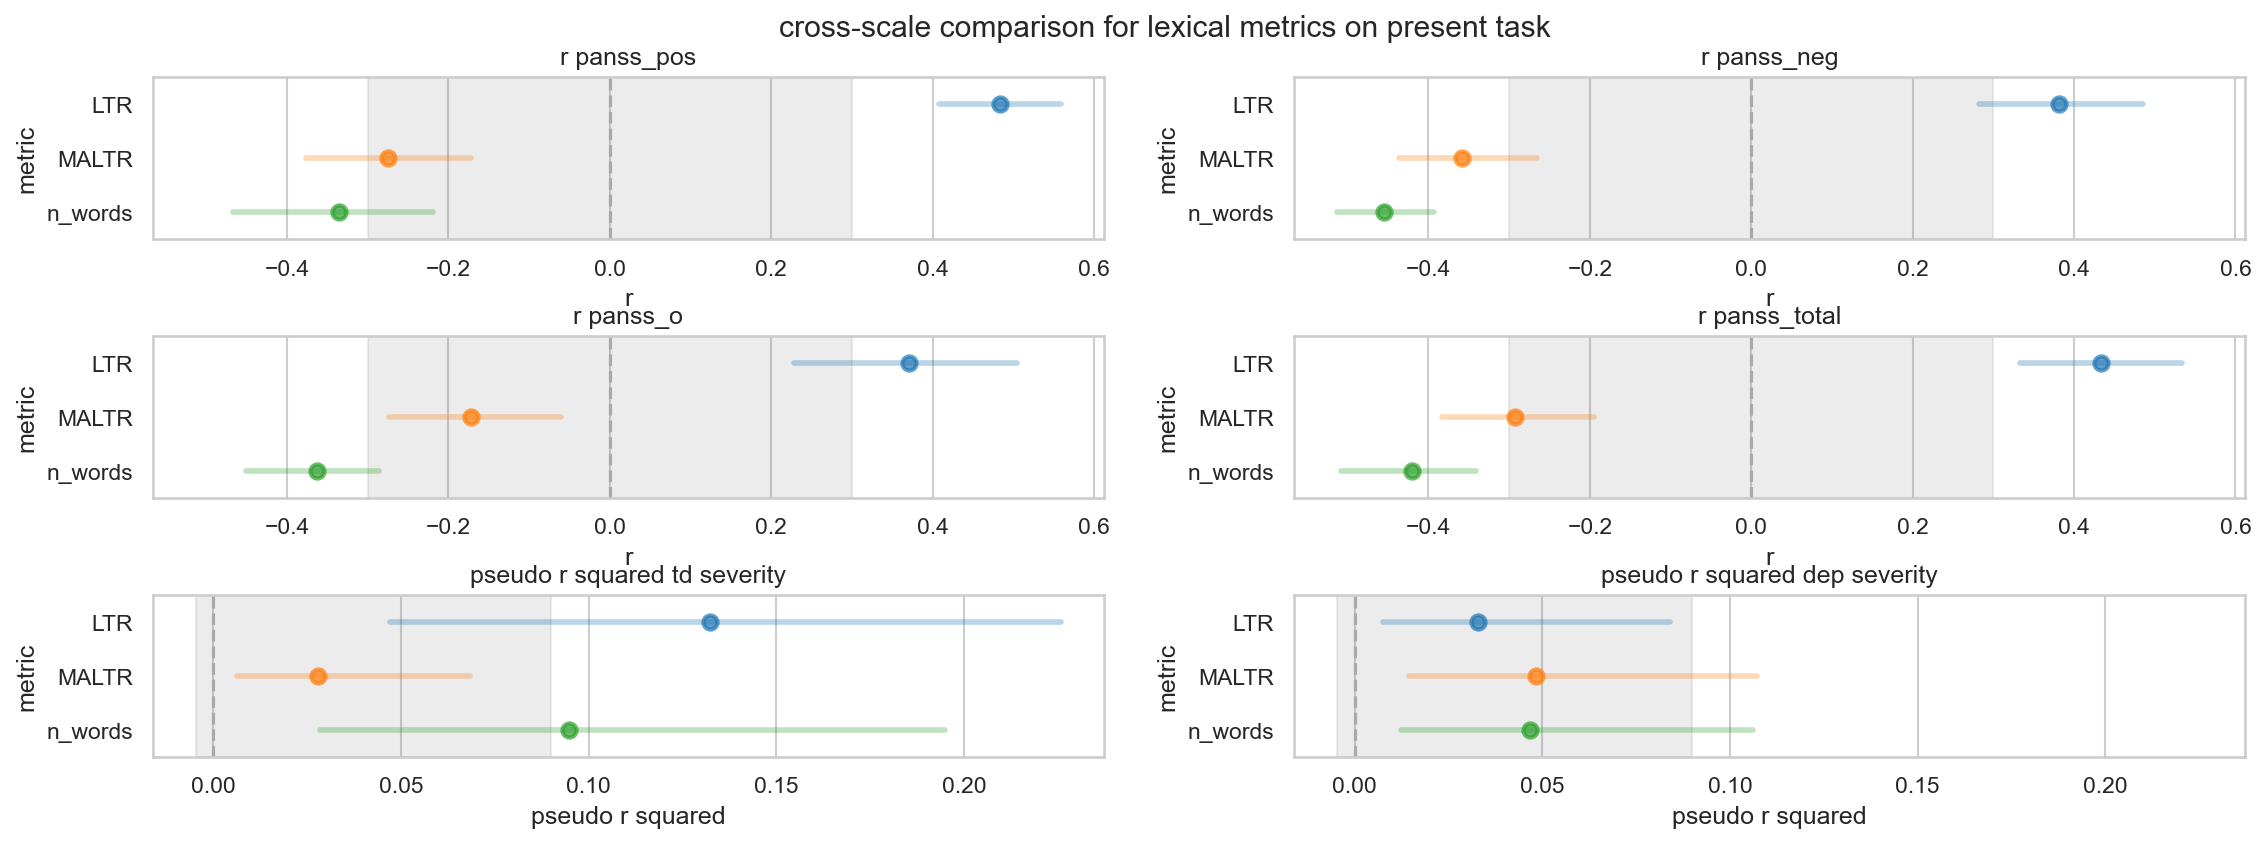
\includegraphics[width=0.9\textwidth, center]{Figures/chapter_4/lexical/ru_present_scale_r.png} 
\captionsetup{width=\textwidth}
\caption[Lexical Metrics: Russian, Present Task]{\label{fig:results:lexical:ru:pr} Pearson's r correlation coefficient and pseudo r squared for each scale for the lexical metrics on the Russian dataset, present task. Grey indicates the values below the 0.3 threshold in absolute value or pseudo r squared below 0.09.}
\end{figure}

Finally, on sportsman task, shown in figure \ref{fig:results:lexical:ru:sp}, LTR also correlated positively with all PANSS subscales and was predictive of TD severity, and word count correlated negatively with all PANSS subscales and was also predictive of TD severity. MALTR did not perform on any of the scales on this task.

\begin{figure}[ht!]
    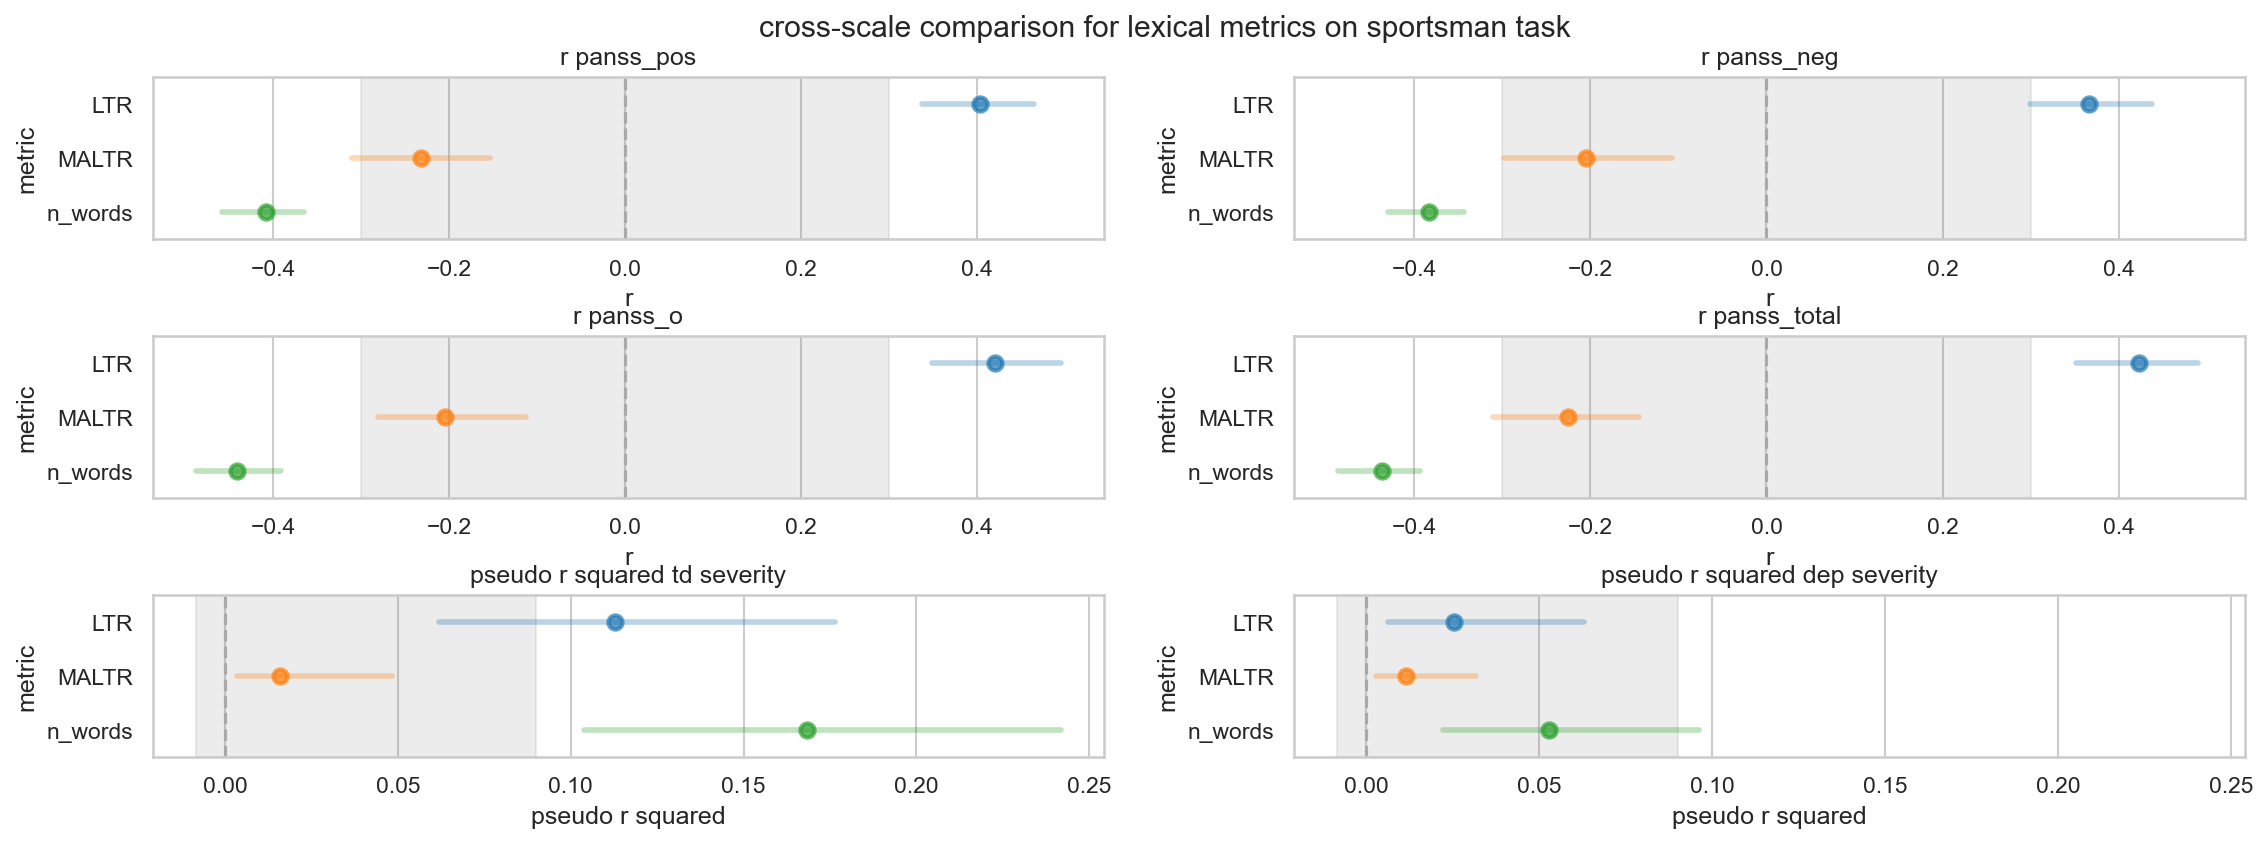
\includegraphics[width=0.9\textwidth, center]{Figures/chapter_4/lexical/ru_sportsman_scale_r.png} 
\captionsetup{width=\textwidth}
\caption[Lexical Metrics: Russian, Sportsman Task]{\label{fig:results:lexical:ru:sp} Pearson's r correlation coefficient and pseudo r squared for each scale for the lexical metrics on the Russian dataset, sportsman task. Grey indicates the values below the 0.3 threshold in absolute value or pseudo r squared below 0.09.}
\end{figure}

Figure \ref{fig:results:lexical:ru:corr_len} shows the strength of correlation with mean sentence length across tasks, indicating that MALTR positively correlated with mean sentence length on all tasks, while word count only does on chair task, and LTR only on sportsman task.

\begin{figure}[ht!]
    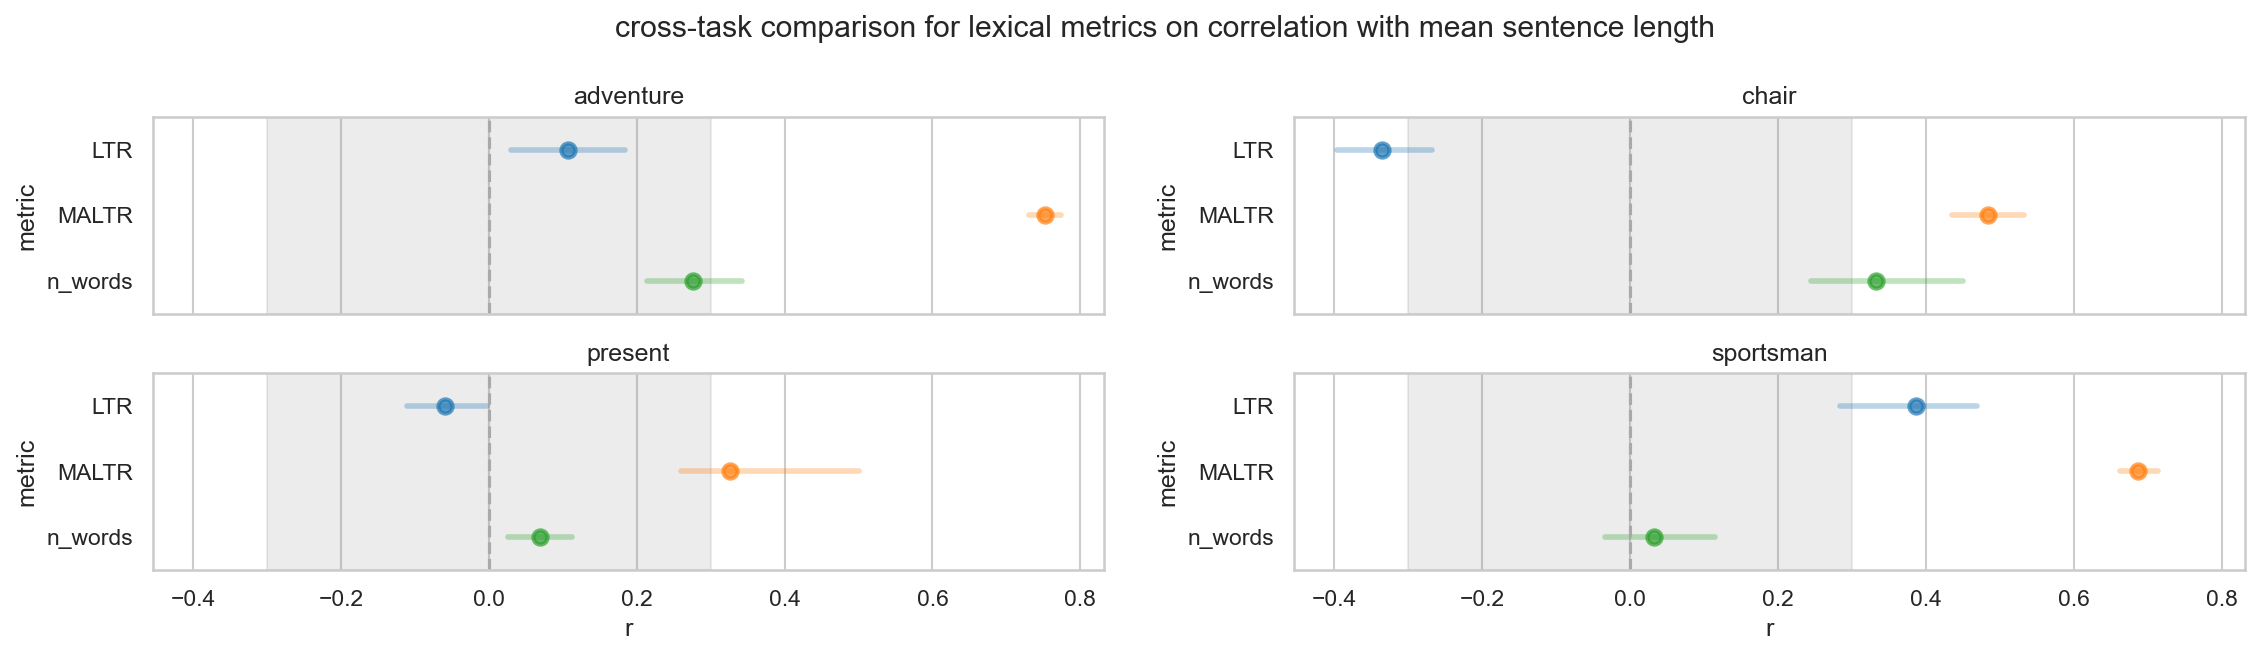
\includegraphics[width=0.9\textwidth, center]{Figures/chapter_4/lexical/ru_corr_len.png} 
\captionsetup{width=\textwidth}
\caption[Lexical Metrics: Russian, Length Correlation]{\label{fig:results:lexical:ru:corr_len} Pearson's r correlation coefficient with mean sentence length for the lexical metrics on the Russian dataset across tasks. Grey indicates the values below 0.3.}
\end{figure}

Overall, on the Russian sample, LTR correlated positively across PANSS subscales but for one task, and word count correlated negatively across PANSS subscales but for one task, while MALTR only performed on two tasks. LTR and word count were also predictive of TD severity on two tasks and of depression severity on one task, while not being overly strongly correlated with mean sentence length.

\subsection{Cross-Linguistic Comparison}
The direction of the correlation for the lexical metrics, was similar between the languages, while the strength of correlation as well as the correlation with mean sentence length differed across scales, tasks, and languages. 


%-----------------------------------
%	section 5
%-----------------------------------
\clearpage
\section{Syntactic Methods}
\label{sec:results:clinical:syntactic}
This section covers the performance of syntactic metrics, including mean, maximal, and minimal sentence length, along with standard deviation in sentence length (mean\_, min\_, max\_, and std\_  sent\_len, respectively), and total sentence count (n sents). Part-of-speech (POS) rates are also tested for the parts-of-speech that were shown to perform in some of the literature, namely: adjectives (ADJ), adverbs (ADV), auxiliary verbs (AUX), coordinating and subordinating conjunctions (CCONJ, SCONJ), determiners (DET), nouns and proper nouns (NOUN, PRPON), pronouns (PRON), particles (PART), and verbs (VERB).

\subsection{German}
The performance of the syntactic metrics on the German sample is shown in figure \ref{fig:results:syntactic:de}. 

\begin{figure}[h!]
    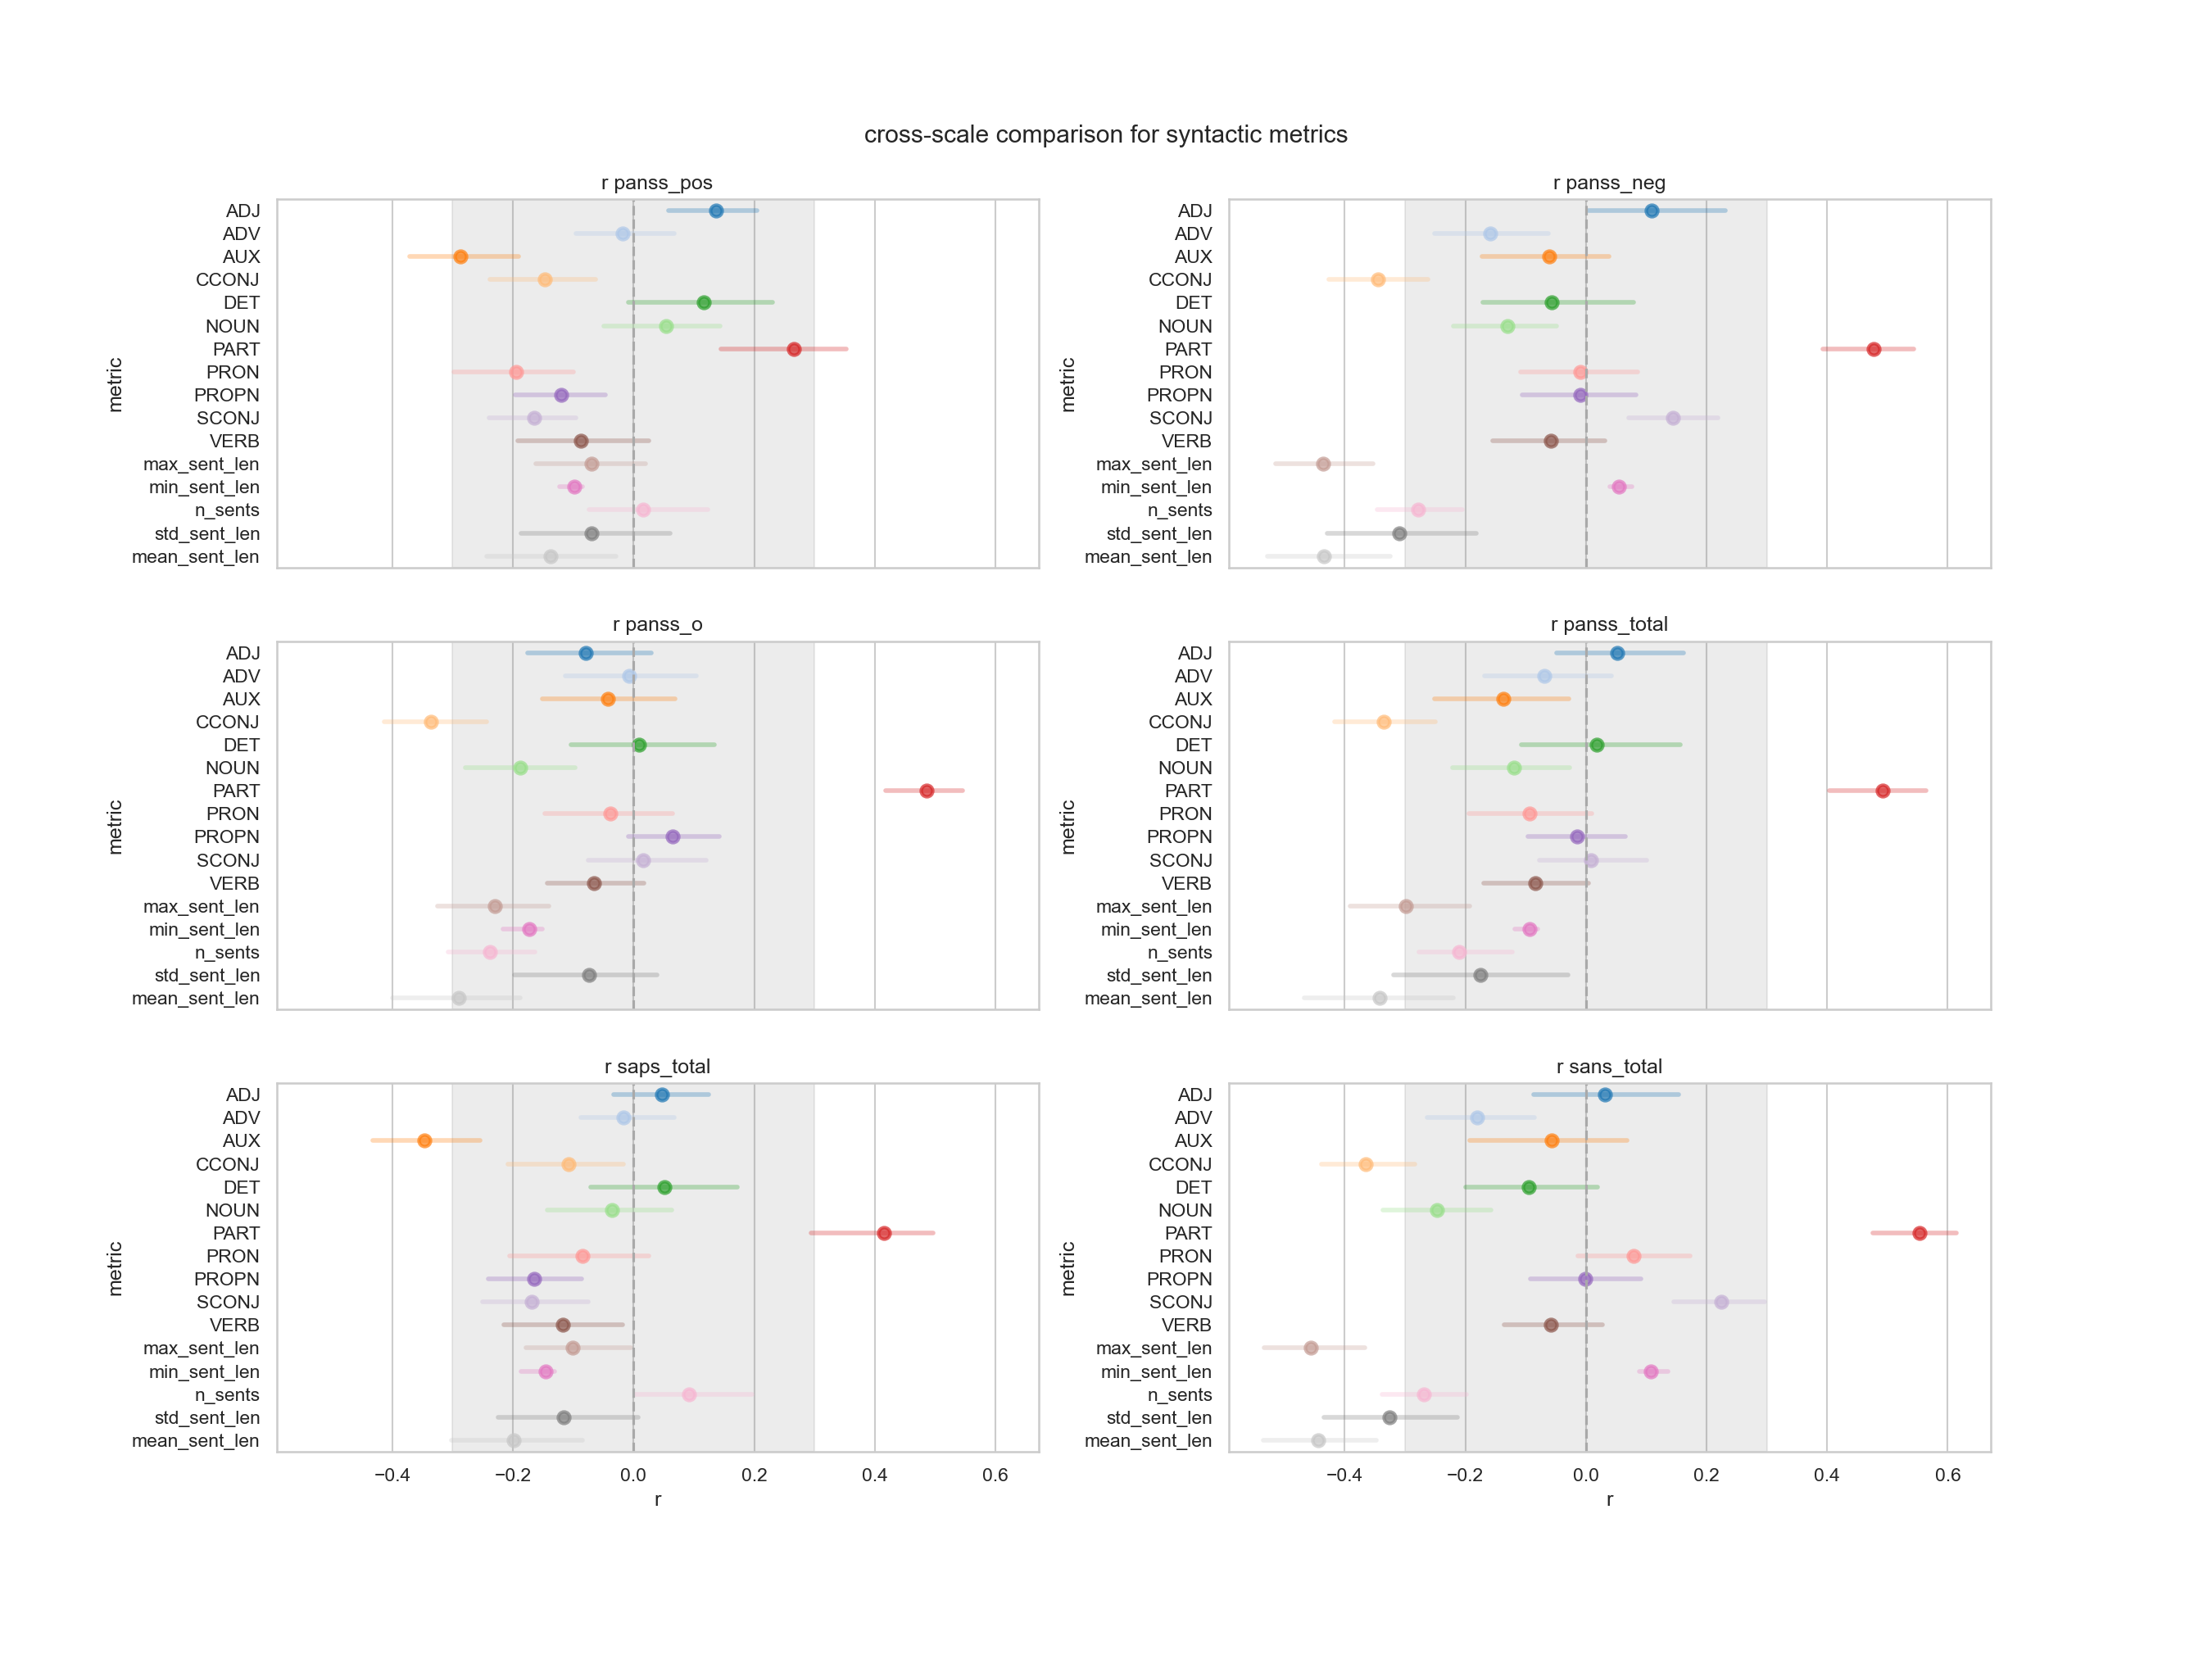
\includegraphics[width=1.2\textwidth, center]{Figures/chapter_4/syntactic/de_scale_r.png} 
\captionsetup{width=\textwidth}
\caption[Syntactic Metrics: German]{\label{fig:results:syntactic:de} Pearson's r correlation coefficient with each scale for the syntactic metrics on the German dataset. Grey indicates the values below the 0.3 threshold in absolute value.}
\end{figure}

Among the POS rate metrics, only PART, AUX, and CCONJ correlated consistently with any of the scales. PART use correlated positively with all scales, but PANSS positive. AUX correlated negatively with all scales, but the positive ones, while CCONJ correlated negatively only with SAPS total score. As for the other syntactic metrics, maximum, mean, and minimal sentence length showed the best performance, as they correlated negatively with all negative scales as well as with PANSS total score, except for minimal sentence length. None of the other metrics correlated with any of the scales.

\clearpage
\begin{figure}[ht!]
    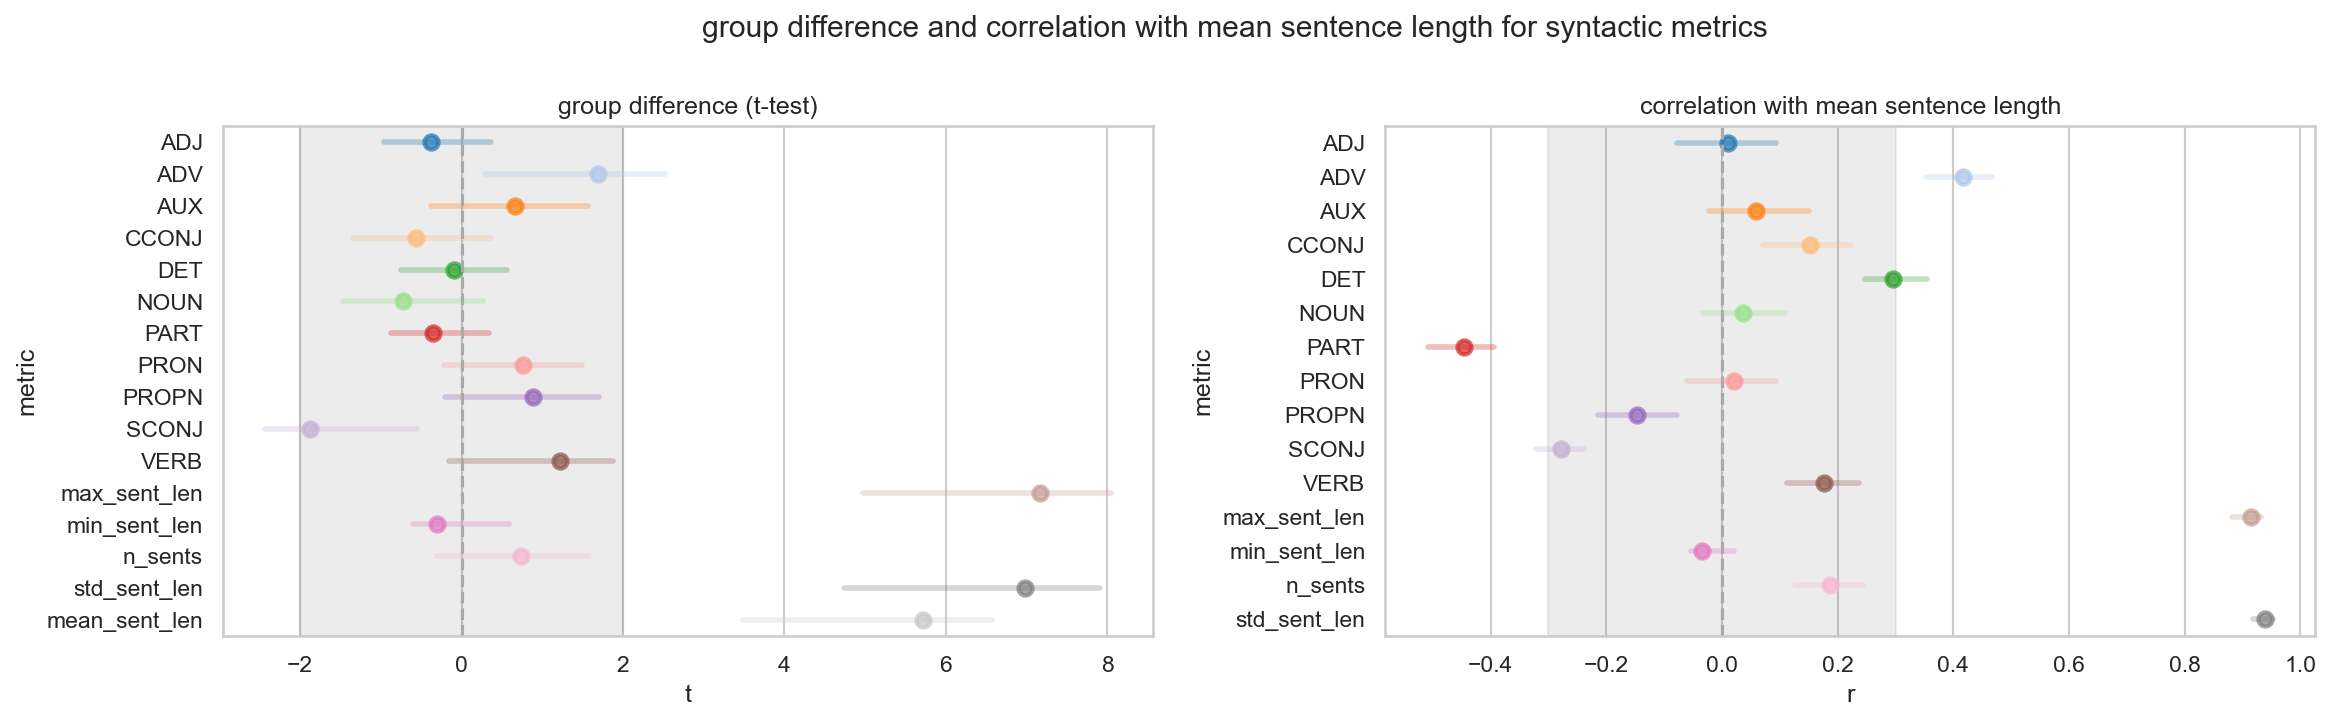
\includegraphics[width=1.1\textwidth, center]{Figures/chapter_4/syntactic/de_t_test_corr_len.png} 
\captionsetup{width=\textwidth}
\caption[Syntactic Metrics: German (T-Test)]{\label{fig:results:syntactic:de:ttest} T-test and Pearson's r correlation coefficient with mean sentence length for the syntactic metrics on the German dataset. Grey indicates the values below 2 for t score and below the 0.3 threshold in absolute value for correlation coefficient.}
\end{figure}


Figure \ref{fig:results:syntactic:de:ttest} compares the strength of the t-test to the corresponding correlation with mean sentence length. Mean sentence length is a reasonable baseline for the German sample, and both maximal and minimal sentence length, as could be expected, correlated strongly with it, somewhat outperforming it on the t-test. PART correlated negatively with mean sentence length, while ADV correlated positively with it.

\clearpage
\subsection{Russian}

Figure \ref{fig:results:syntactic:ru:ad} shows the performance of the syntactic metrics on the adventure task, and the only metric that correlated with any of the symptom scales is the total number of sentences, which correlated negatively with general symptoms and total PANSS score.

\begin{figure}[ht!]
    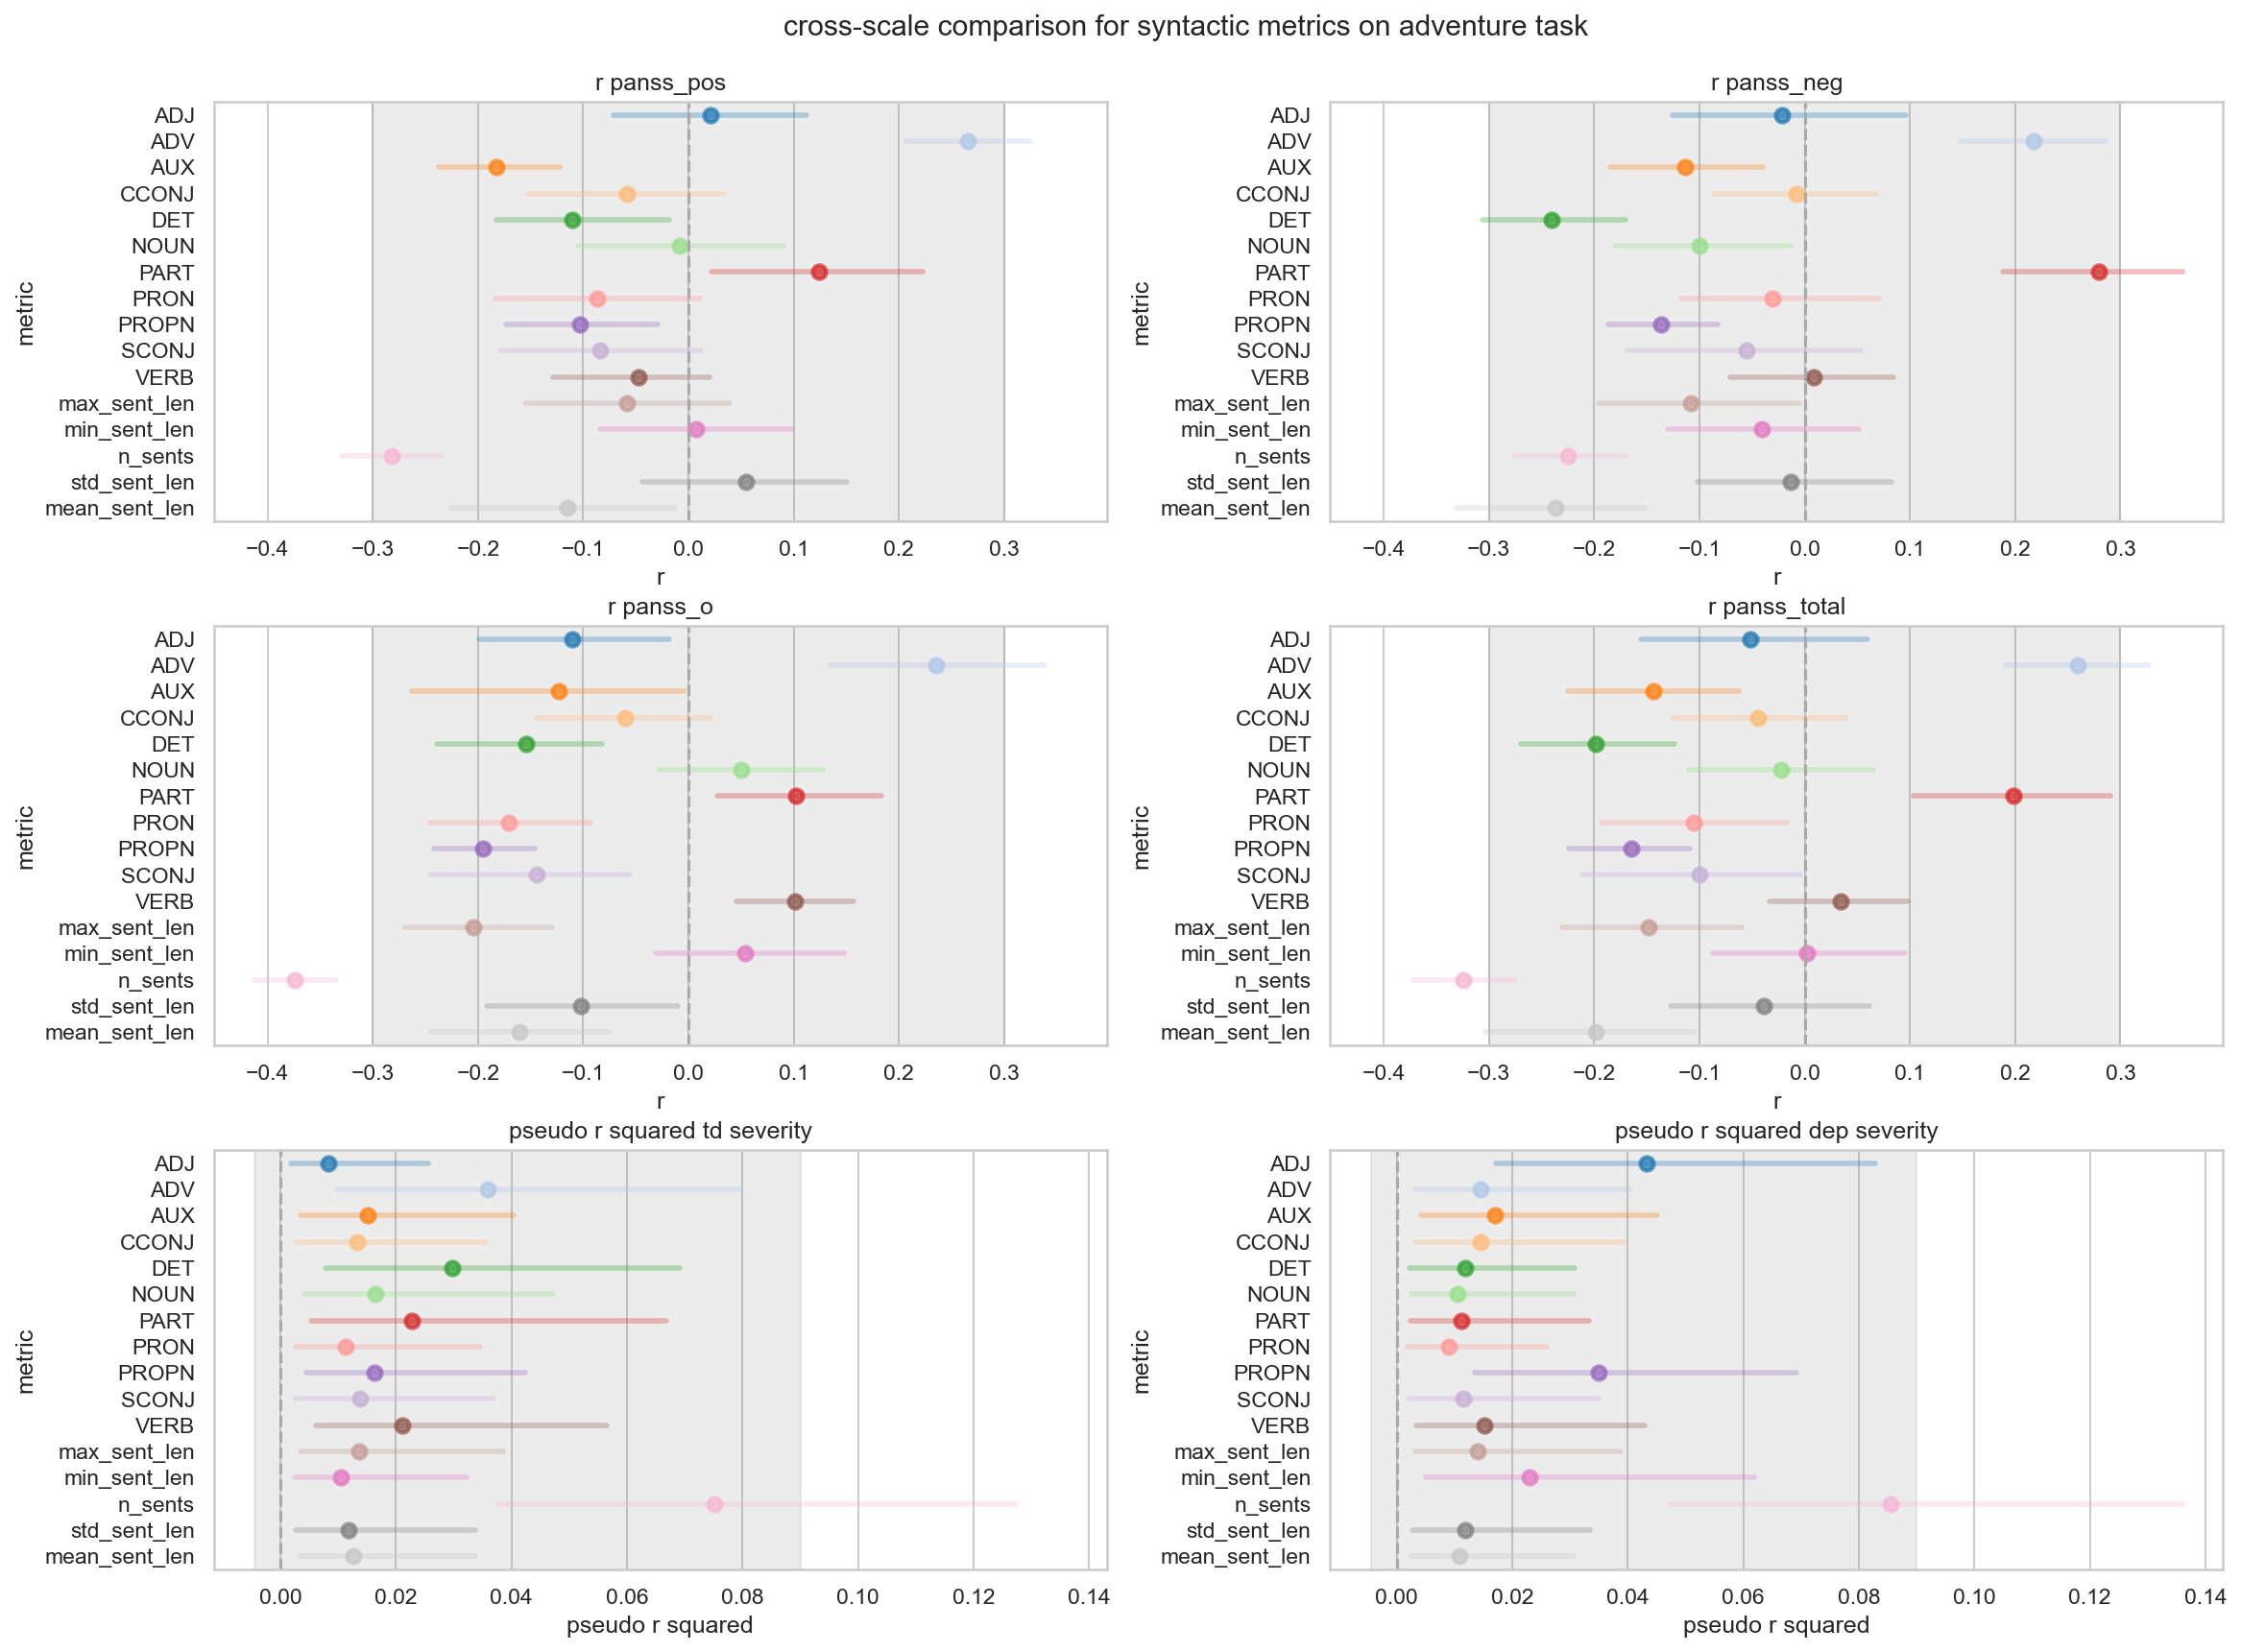
\includegraphics[width=1.1\textwidth, center]{Figures/chapter_4/syntactic/ru_adventure_scale_r.png} 
\captionsetup{width=\textwidth}
\caption[Syntactic Metrics: Russian, Adventure Task]{\label{fig:results:syntactic:ru:ad} Pearson's r correlation coefficient and pseudo r squared for each scale for the syntactic metrics on the Russian dataset, adventure task. Grey indicates the values below the 0.3 threshold in absolute value or pseudo r squared below 0.09.}
\end{figure}

\clearpage
Figure \ref{fig:results:syntactic:ru:ch} shows the performance of the syntactic metrics on the chair task. Among the parts of speech, PART rate correlated with all PANSS subscales, and NOUN rate with all but the general symptoms subscale. These two metrics were also the only ones performing well in TD severity detection. The mean sentence length correlated with all PANSS subscales as well as predicted depression severity along with maximal sentence length. The total number of sentences correlated with all PANSS subscales but PANSS negative.

\begin{figure}[ht!]
    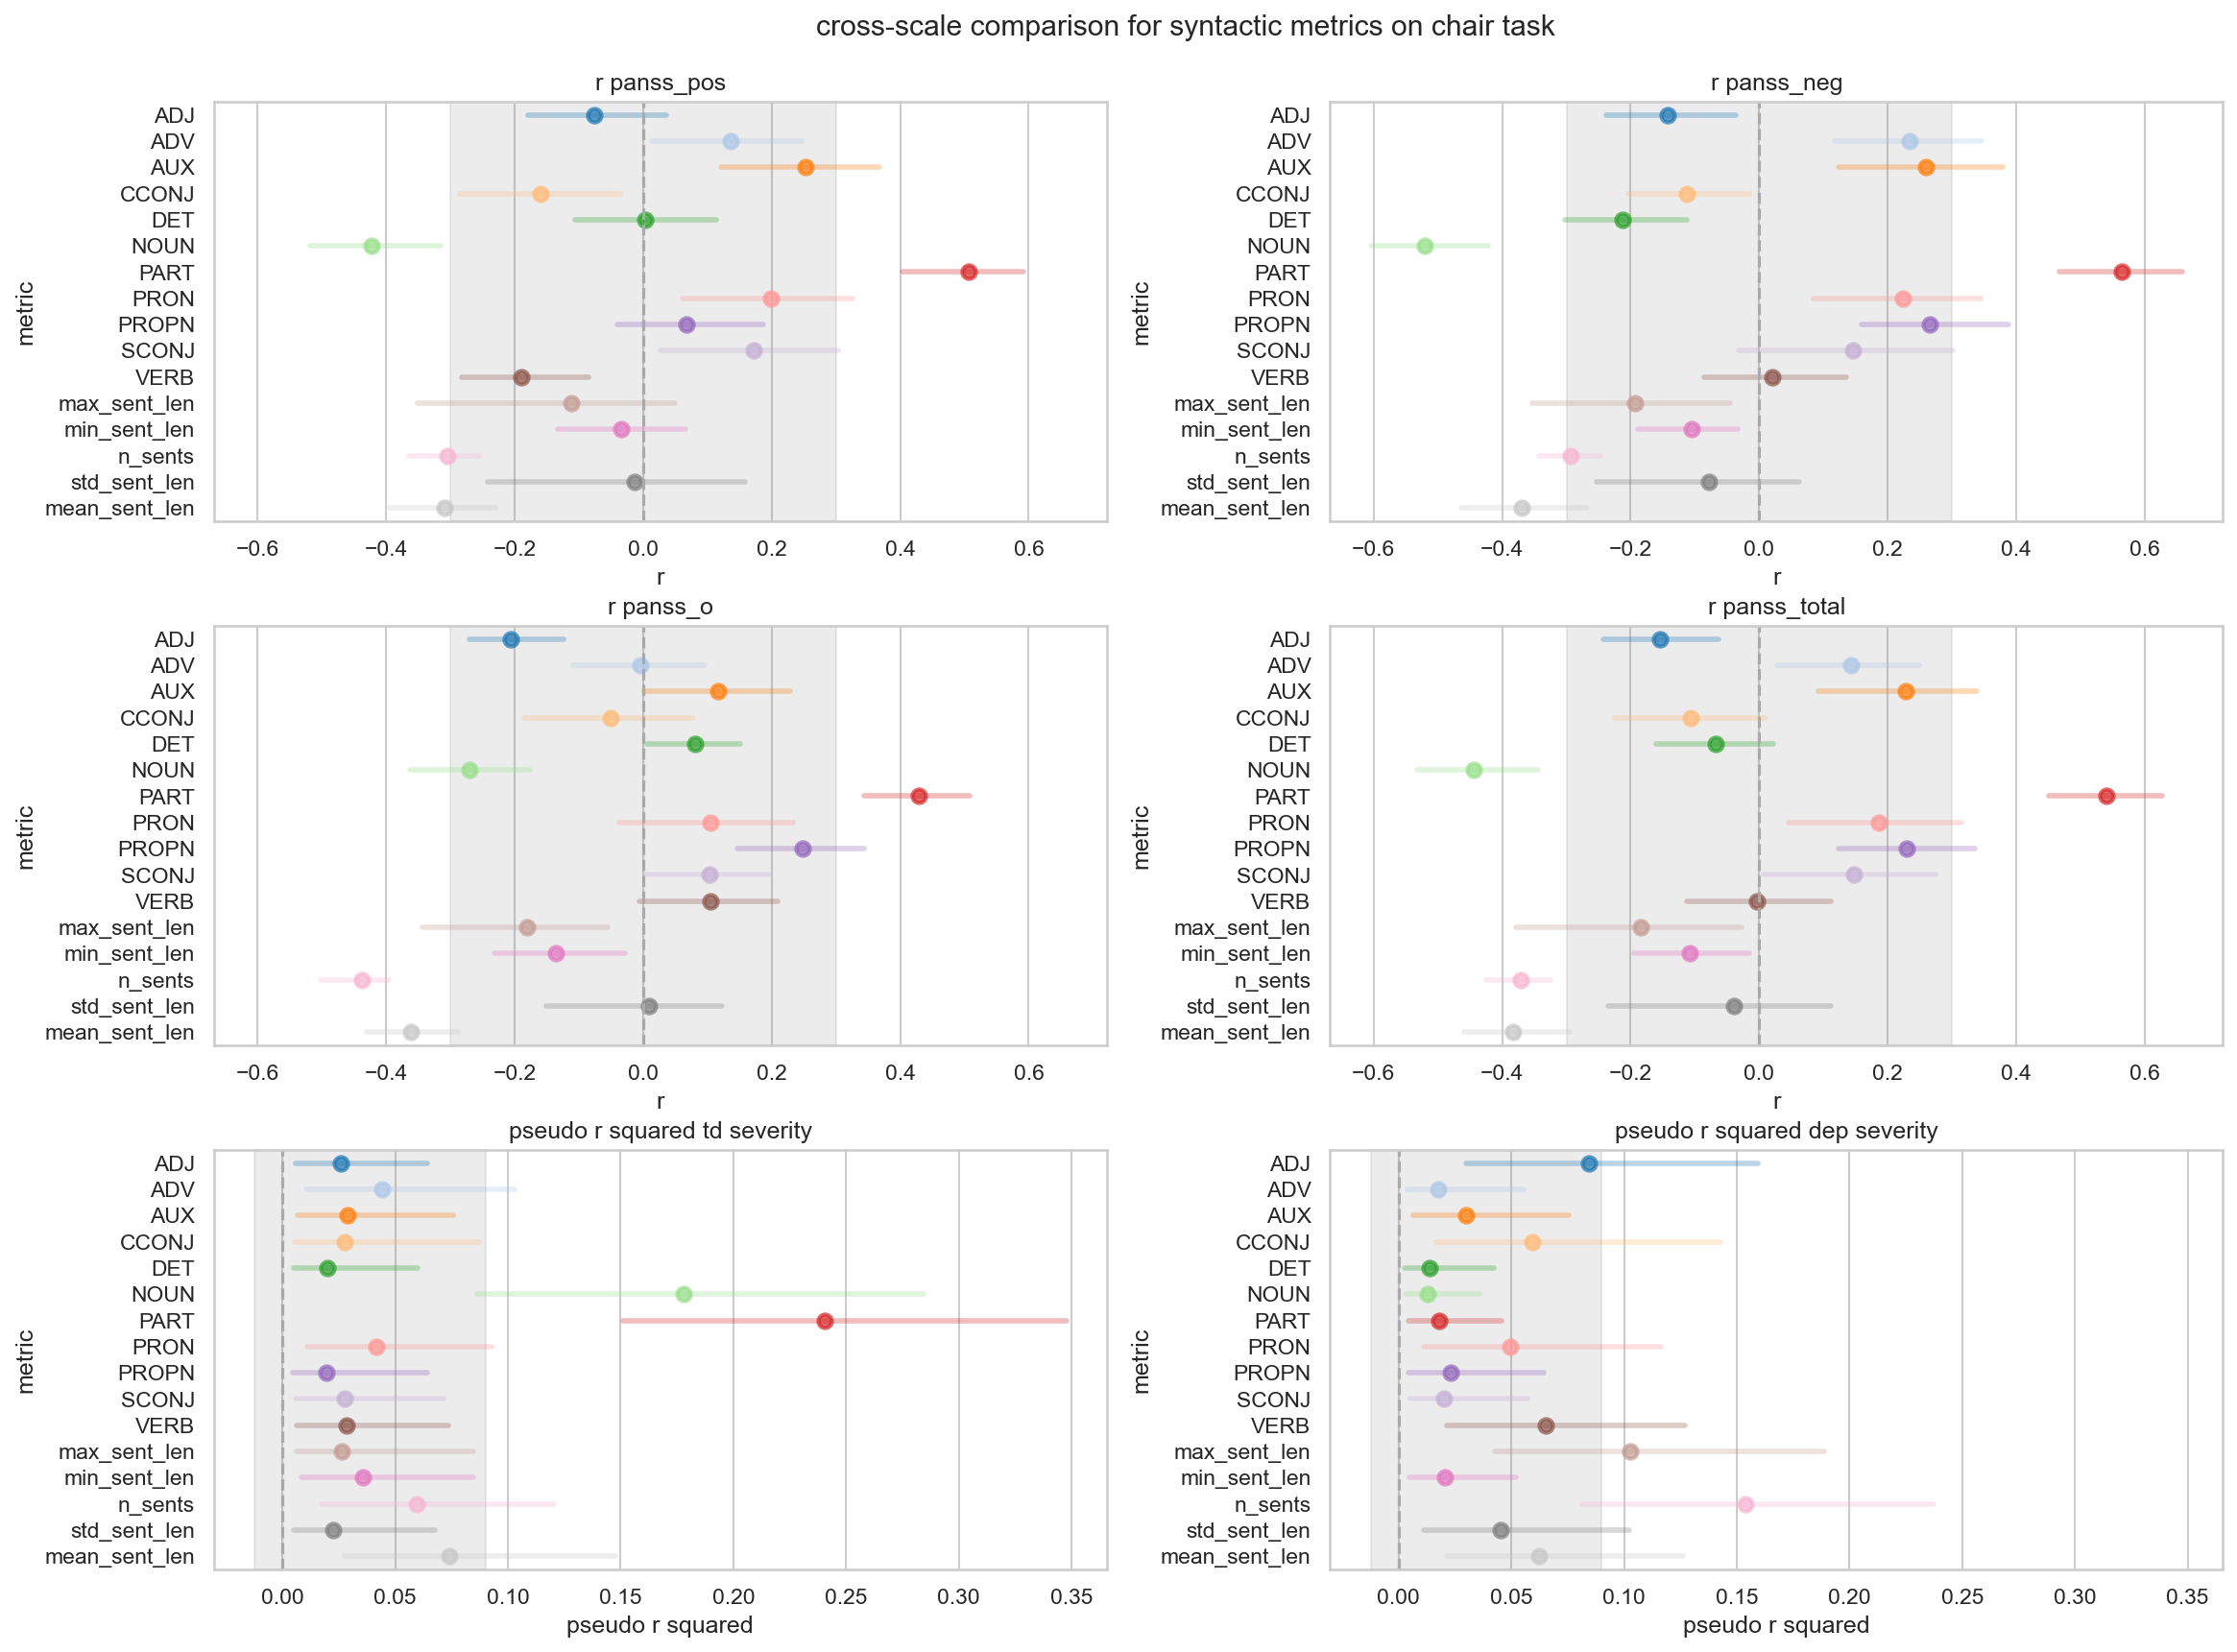
\includegraphics[width=1.1\textwidth, center]{Figures/chapter_4/syntactic/ru_chair_scale_r.png} 
\captionsetup{width=\textwidth}
\caption[Syntactic Metrics: Russian, Chair Task]{\label{fig:results:syntactic:ru:ch} Pearson's r correlation coefficient and pseudo r squared for each scale for the syntactic metrics on the Russian dataset, chair task. Grey indicates the values below the 0.3 threshold in absolute value or pseudo r squared below 0.09.}
\end{figure}

\clearpage
Figure \ref{fig:results:syntactic:ru:pr} shows the performance of the syntactic metrics on the present task. PART rate correlated positively with PANSS positive and total scores, DET rate correlated negatively with PANSS negative and total scores, and CCONJ rate correlated negatively with PANSS general only. The total number of sentences correlated negatively with PANSS negative only, while mean sentence length did so with all PANSS scales but the positive. Maximal sentence length and the standard deviation correlated negatively with all PANSS scales and also performed well in TD severity detection, largely outperforming mean sentence length.

\begin{figure}[ht!]
    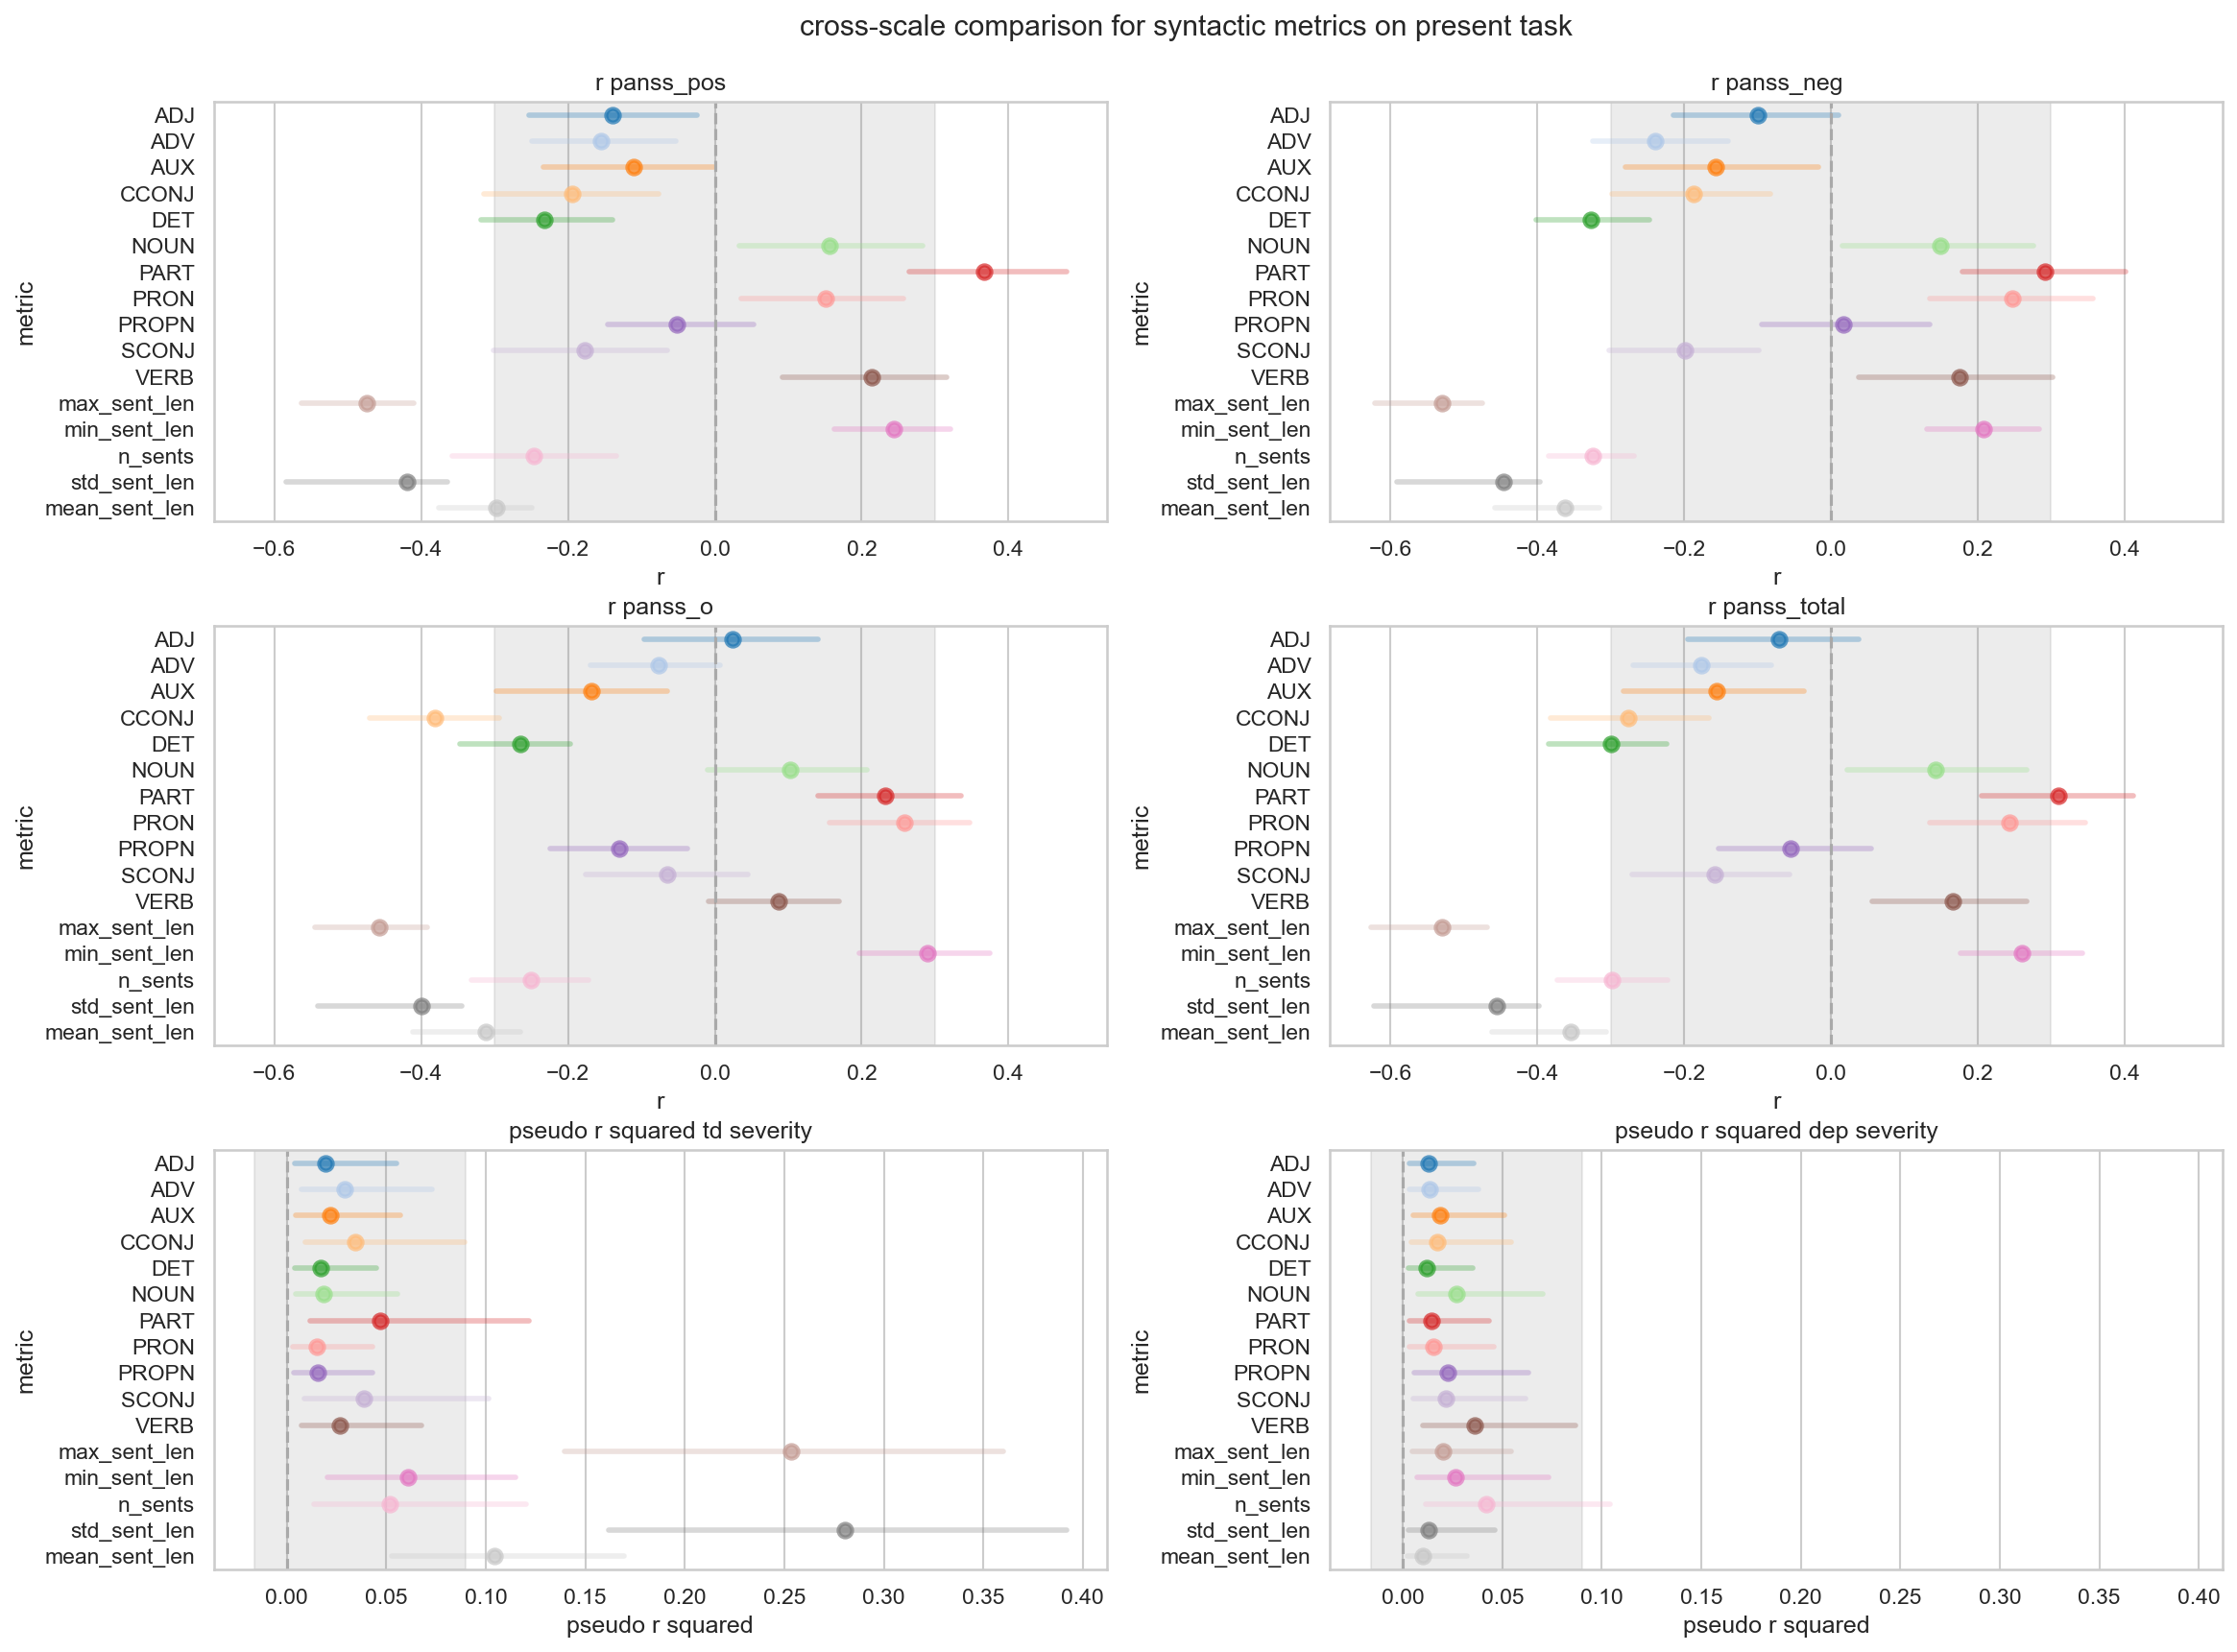
\includegraphics[width=1.1\textwidth, center]{Figures/chapter_4/syntactic/ru_present_scale_r.png} 
\caption[Syntactic Metrics: Russian, Present Task]{\label{fig:results:syntactic:ru:pr} Pearson's r correlation coefficient and pseudo r squared for each scale for the syntactic metrics on the Russian dataset, present task. Grey indicates the values below the 0.3 threshold in absolute value or pseudo r squared below 0.09.}
\end{figure}

\clearpage
Figure \ref{fig:results:syntactic:ru:sp} shows the performance of the syntactic metrics on the sportsman task. On this task, PART correlated positively only with PANSS positive, while maximal sentence length correlated with it negatively. The number of sentences on the other hand correlated negatively with all PANSS scales and was also the only metric sensitive to TD severity.

\begin{figure}[ht!]
    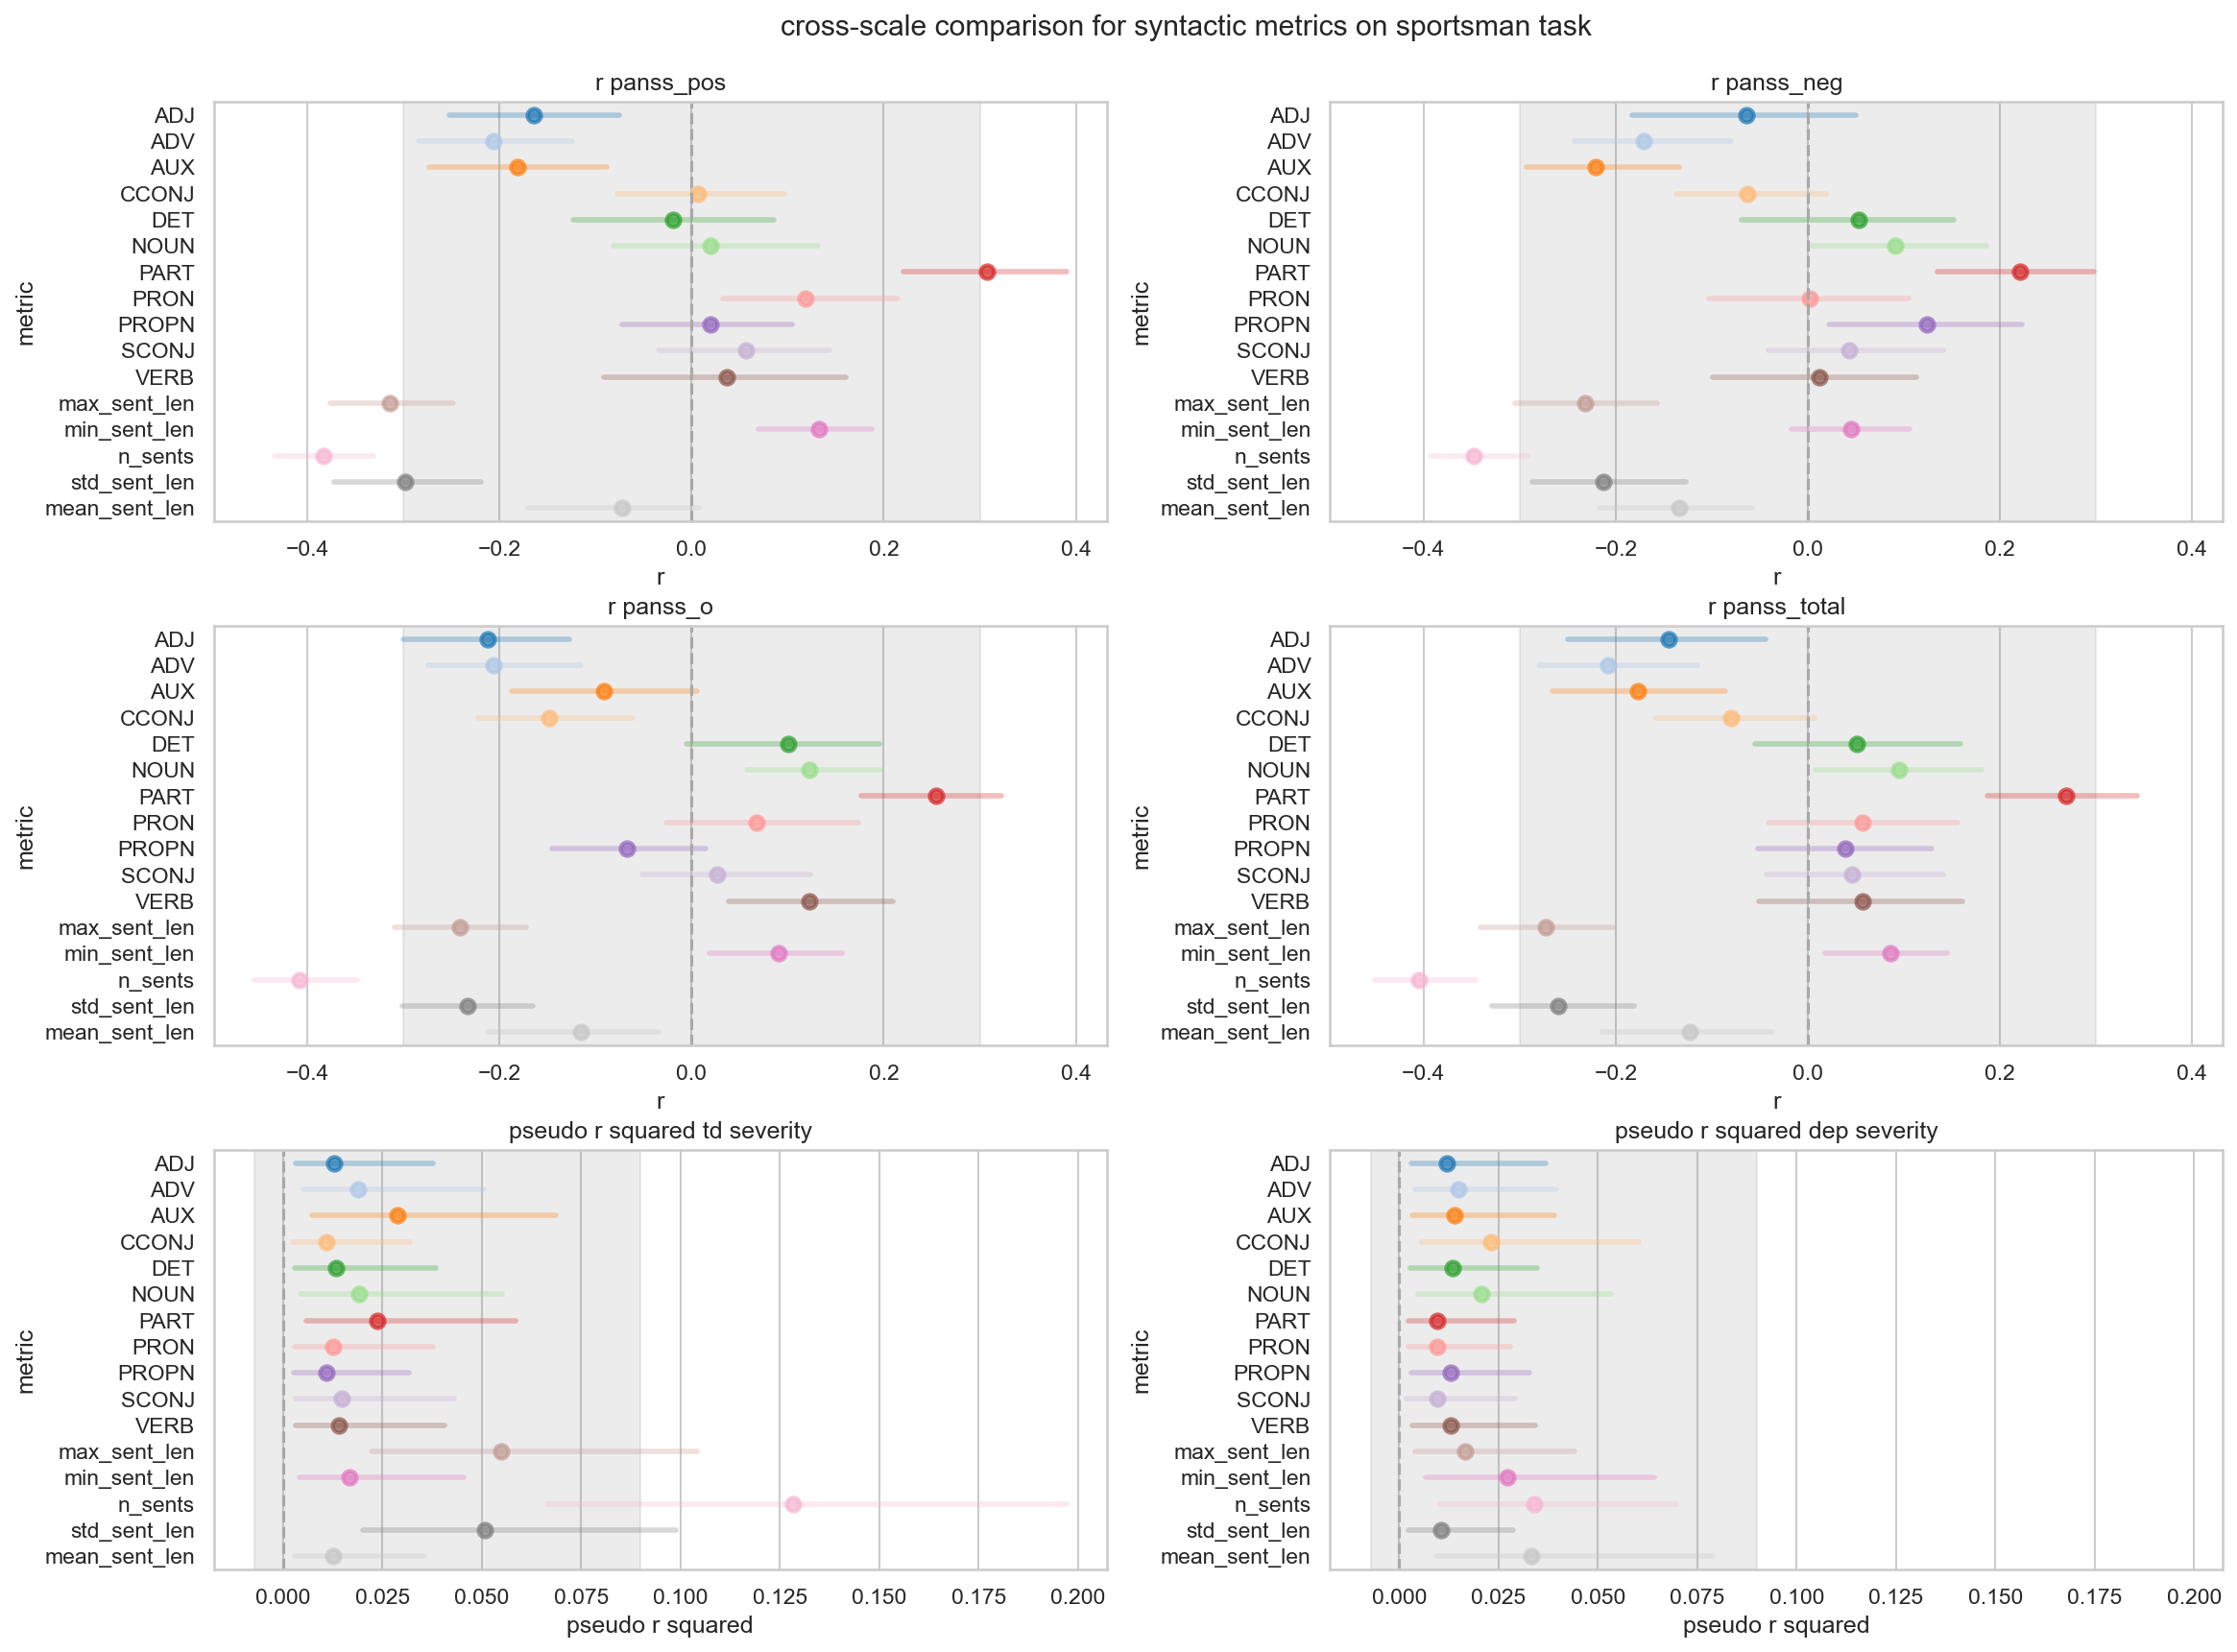
\includegraphics[width=1.1\textwidth, center]{Figures/chapter_4/syntactic/ru_sportsman_scale_r.png} 
\captionsetup{width=\textwidth}
\caption[Syntactic Metrics: Russian, Sportsman Task]{\label{fig:results:syntactic:ru:sp} Pearson's r correlation coefficient and pseudo r squared for each scale for the syntactic metrics on the Russian dataset, sportsman task. Grey indicates the values below the 0.3 threshold in absolute value or pseudo r squared below 0.09.}
\end{figure}

\clearpage
Figure \ref{fig:results:syntactic:ru:corr_len} shows the strength of correlation with mean sentence length across tasks. As could be expected, on all tasks, maximal, standard deviation, and minimal sentence length correlated positively with the mean. VERB rate correlated negatively with mean sentence length on sportsman and adventure tasks, and ADV did so on chair task, while ADJ correlated positively with mean sentence length on all tasks present, and NOUN did so on chair task. Importantly, it is on the chair task that NOUN performed well. 

\begin{figure}[ht!]
    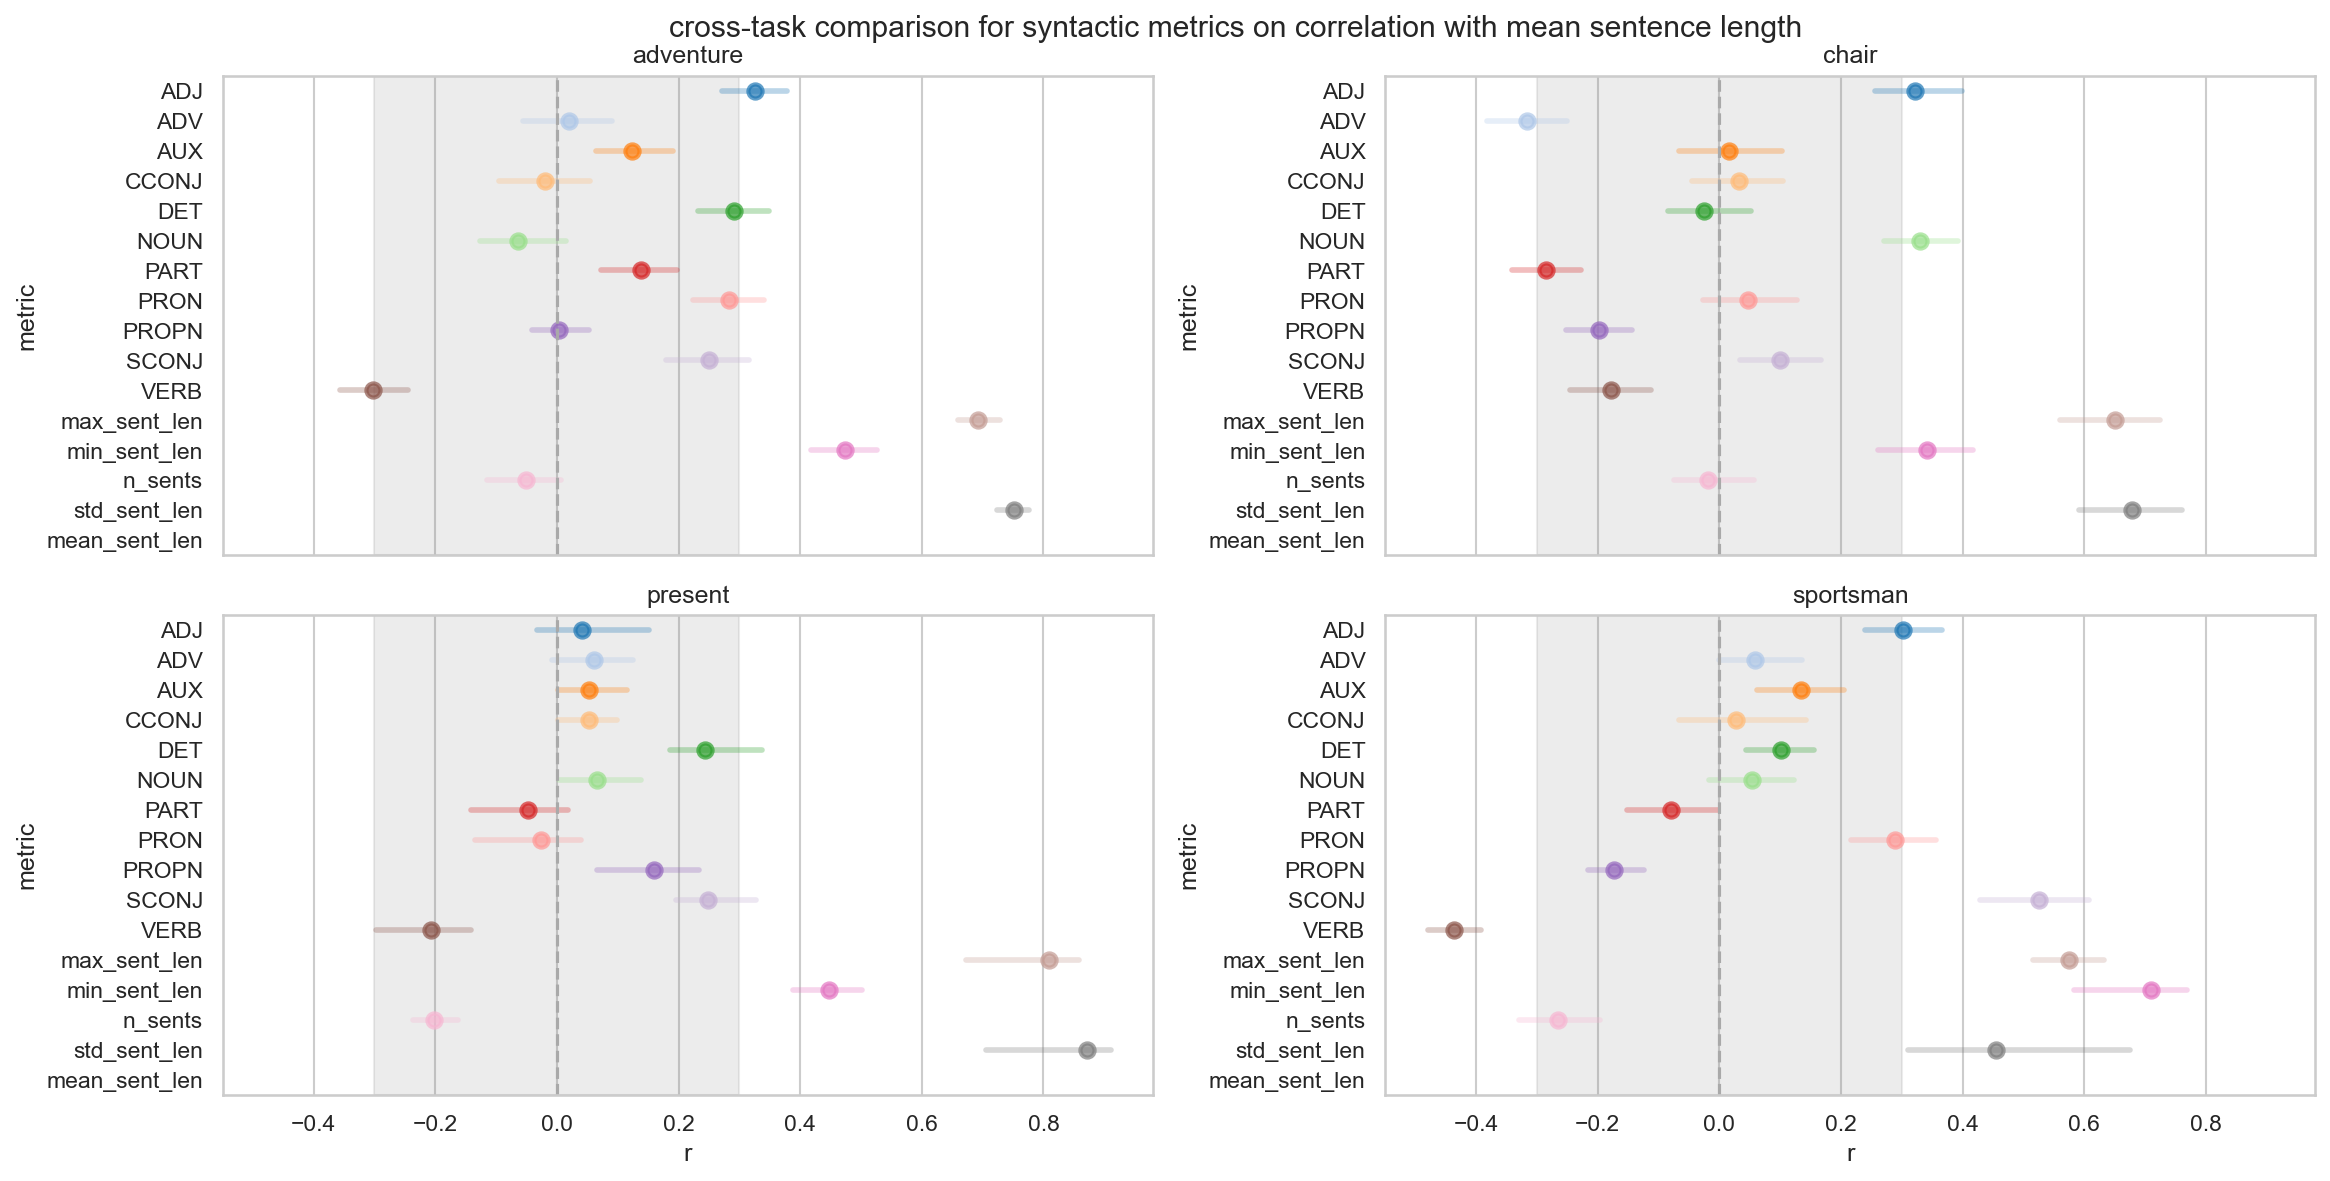
\includegraphics[width=1.1\textwidth, center]{Figures/chapter_4/syntactic/ru_corr_len.png} 
\captionsetup{width=\textwidth}
\caption[Syntactic Metrics: Russian, Length Correlation]{\label{fig:results:syntactic:ru:corr_len} Pearson's r correlation coefficient with mean sentence length for the syntactic metrics on the Russian dataset across tasks. Grey indicates the values below 0.3.}
\end{figure}

Overall, on the Russian sample, the number of sentences was the strongest metric, being the only one, that correlated with symptom scales on all tasks. The rate of PART was positively correlated with symptom severity on three of the four tasks. As could be expected, mean sentence length served as a good baseline on only two of the tasks (chair and	present), and maximal sentence length performed on the same tasks, though it correlated with fewer subscales that mean sentence length. As for, CCONJ, DET, and NOUN rates, each only performed on one of the tasks, and the same is true of standard deviation in mean sentence length.

\subsection{Cross-Linguistic Comparison}
In both languages, PART rate correlated positively with PANSS scales, and similarly in both languages mean, maximal, and standard deviation sentence length correlated negatively with PANSS scales, with mean sentence length performing better on the German sample, as could be expected. CCONJ rate correlated negatively both on the German and the Russian samples, though for the latter only on one scale for one task. AUX rate correlated negatively only on the German sample, and NOUN and DET did so only on the Russian sample, both on only one task. Similarly, the number of sentences correlated negatively with PANSS scales only on the Russian sample.



%-----------------------------------
%	section 6
%-----------------------------------
\clearpage
\section{Graph-Based Methods}
\label{sec:results:clinical:graph}
This section covers the performance of co-occurrence graph-based metrics, number of nodes (N), number of edges (E), largest connected component (LCC), largest strongly connected component (LSC), number of parallel edges (PE), number of loops of length one (repeated lemmas), two, and three (L1, L2, L3), average node degree (degree average), and standard deviation in the node degree (degree std).  


\subsection{German}
Among the graph metrics, shown in figure \ref{fig:results:graph:de}, four correlated negatively with negative symptom scales, as well as PANSS general and total scores, namely, the largest connected and strongly connected component size as well as the number of nodes and edges. 

\begin{figure}[h!]
    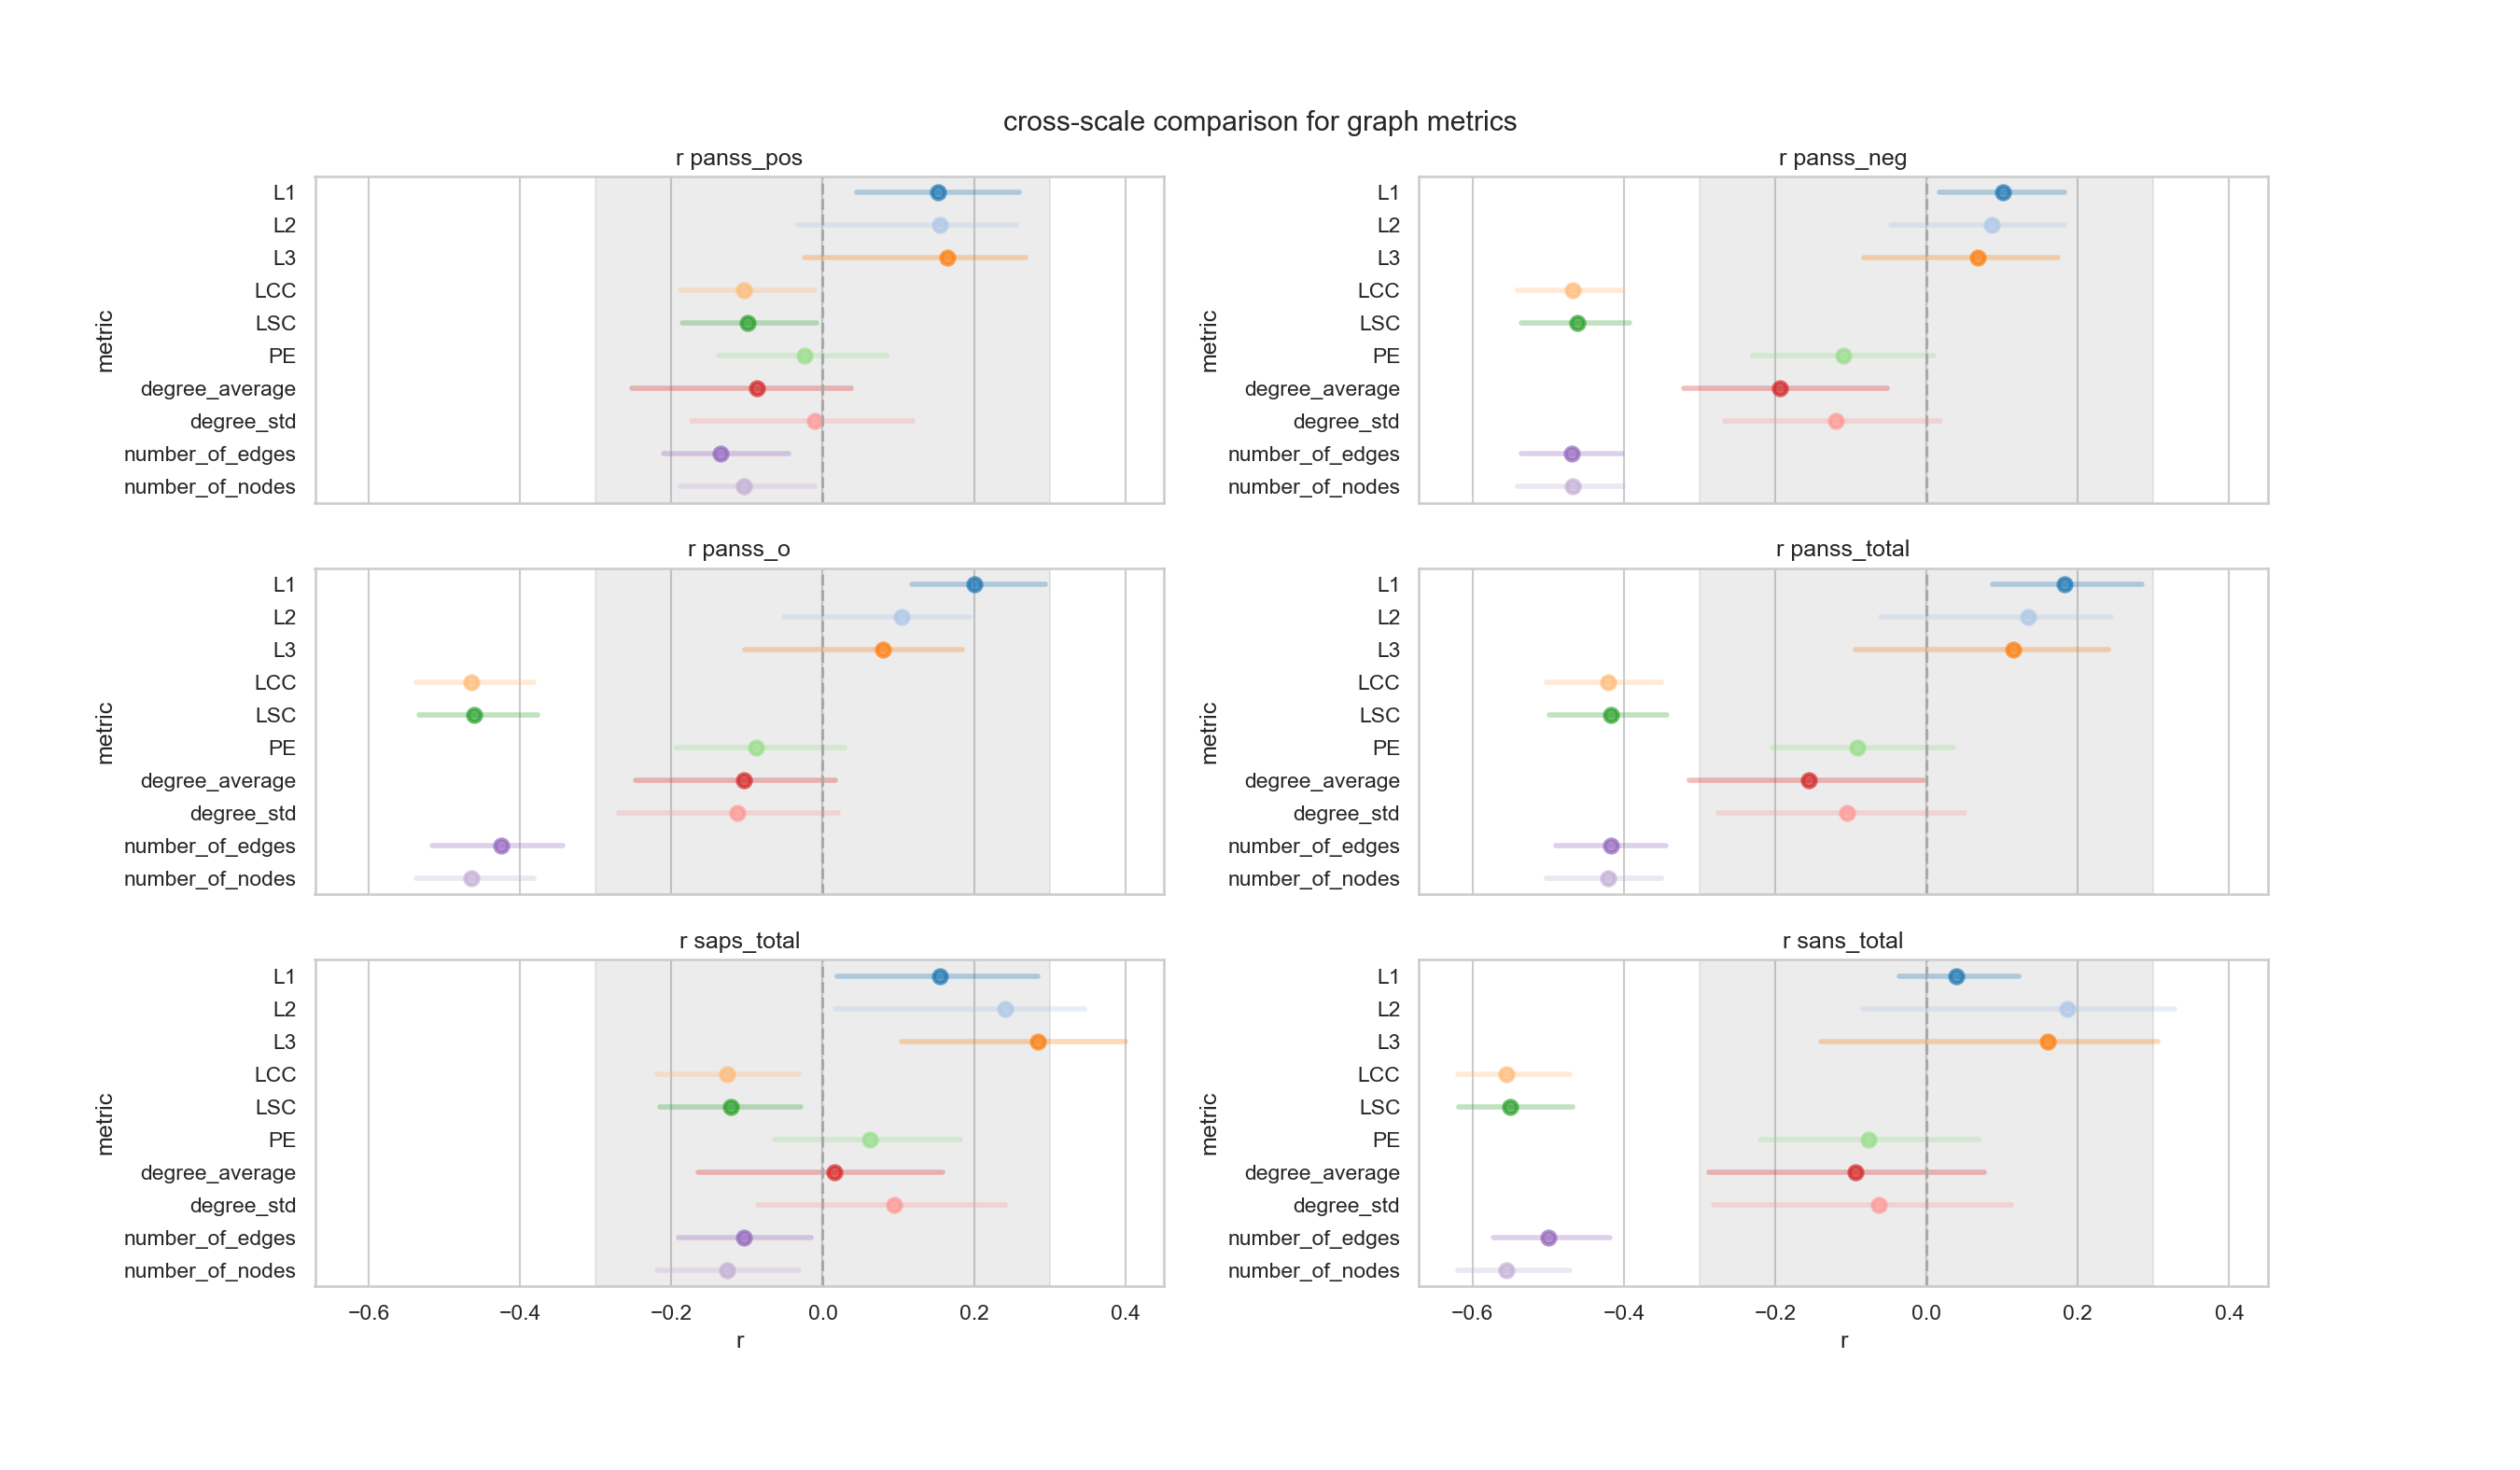
\includegraphics[width=1.2\textwidth, center]{Figures/chapter_4/graph/de_scale_r.png} 
\captionsetup{width=\textwidth}
\caption[Graph Metrics: German]{\label{fig:results:graph:de} Pearson's r correlation coefficient with each scale for the graph-based metrics on the German dataset. Grey indicates the values below the 0.3 threshold in absolute value.}
\end{figure}

Figure \ref{fig:results:graph:de:ttest} shows the strength of correlation with mean sentence length and the power of bidirectional t-test, with the patterns corresponding very closely between the two graphs. The metric values were calculated for moving window of size 100, to avoid direct correlation with verbosity, yet there was still a significant correlation with mean sentence length for all the metrics that performed well on t-test and the psychiatric scales, i.e. LCC, LSC, N, and E. 

\begin{figure}[ht!]
    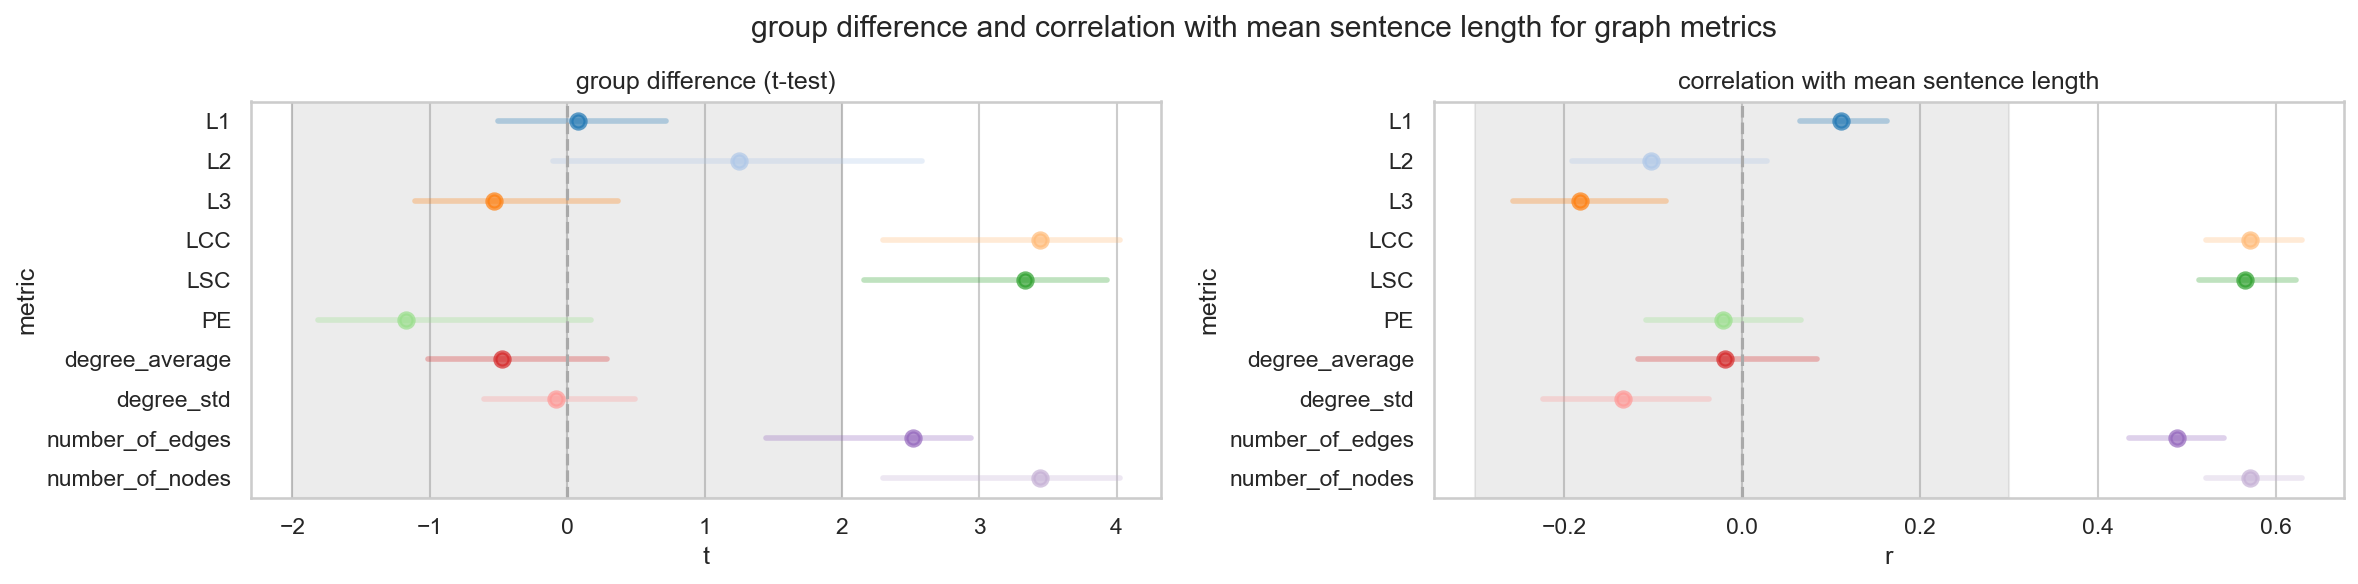
\includegraphics[width=\textwidth, center]{Figures/chapter_4/graph/de_t_test_corr_len.png} 
\captionsetup{width=\textwidth}
\caption[Graph Metrics: German (T-Test)]{\label{fig:results:graph:de:ttest} T-test and Pearson's r correlation coefficient with mean sentence length for the graph-based metrics on the German dataset. Grey indicates the values below 2 for t score and below the 0.3 threshold in absolute value for correlation coefficient.}
\end{figure}

\clearpage
\subsection{Russian}
Figure \ref{fig:results:graph:ru:ad} shows the performance of graph-based metrics on adventure task. The largest connected and strongly connected component size as well as the number of nodes and edges correlated negatively with PANSS general and total scores, and all of these but the number of edges also correlated with PANSS negative.

\begin{figure}[ht!]
    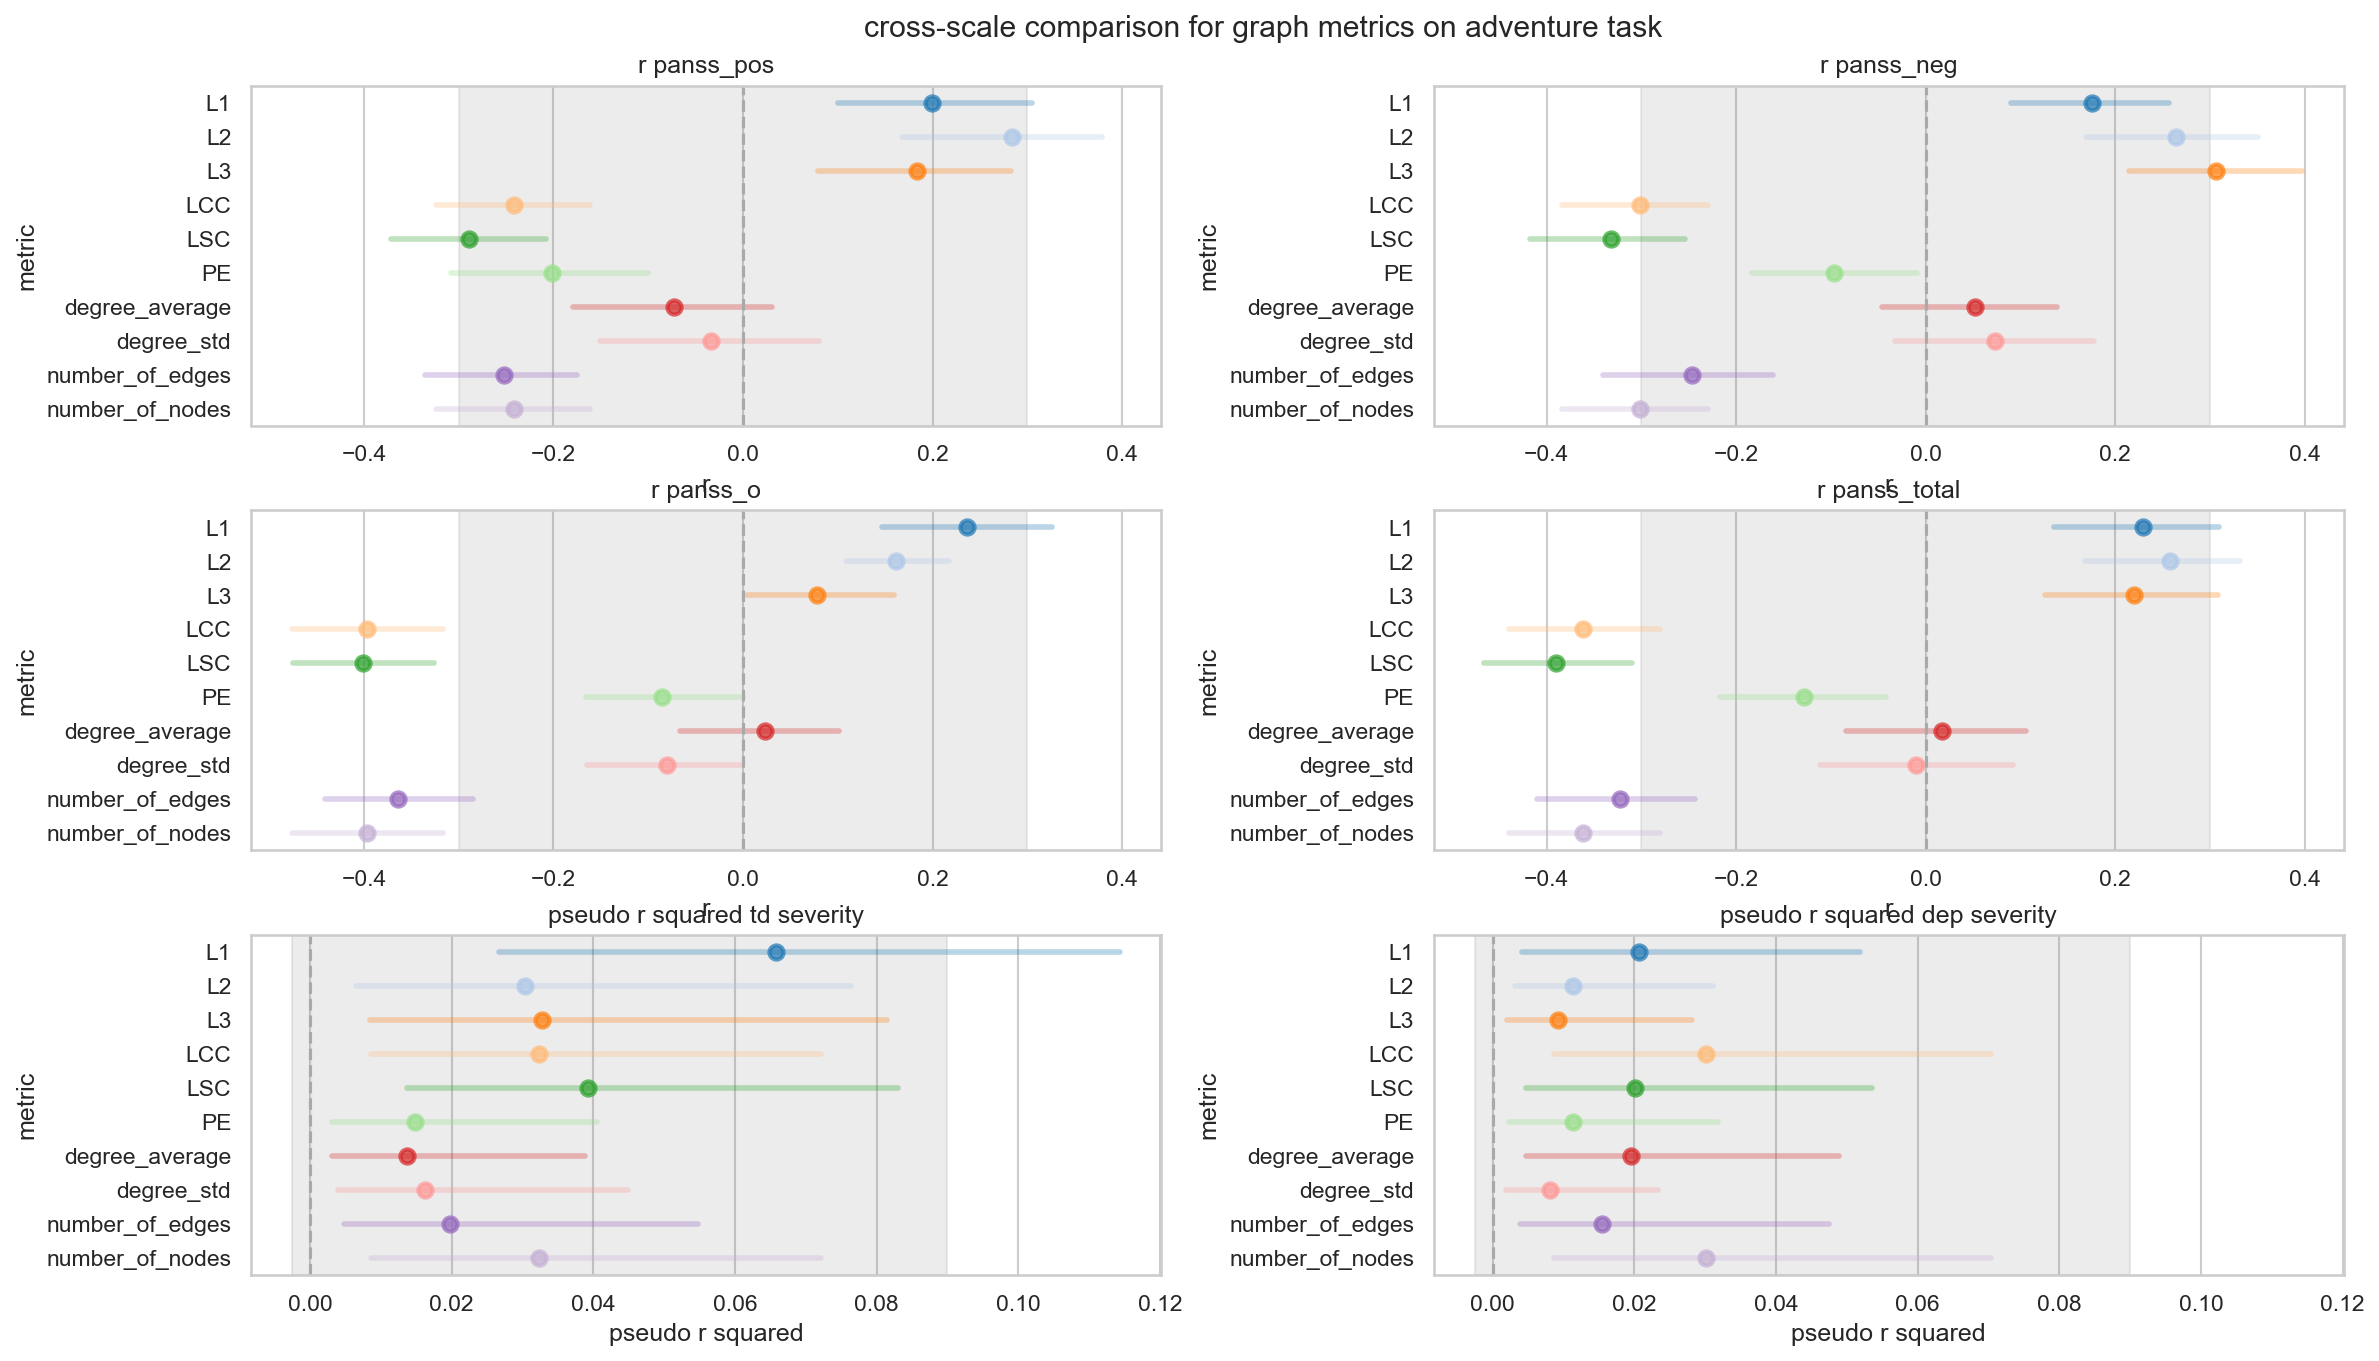
\includegraphics[width=1.1\textwidth, center]{Figures/chapter_4/graph/ru_adventure_scale_r.png} 
\captionsetup{width=\textwidth}
\caption[Graph Metrics: Russian, Adventure Task]{\label{fig:results:graph:ru:ad} Pearson's r correlation coefficient and pseudo r squared for each scale for the graph-based metrics on the Russian dataset, adventure task. Grey indicates the values below the 0.3 threshold in absolute value or pseudo r squared below 0.09.}
\end{figure}

\clearpage
Figure \ref{fig:results:graph:ru:ch} shows the performance of graph-based metrics on chair task. The largest connected and strongly connected component size as well as the number of nodes and edges correlated negatively with all PANSS scales. L3 correlated positively with all PANSS scales and was predictive of TD severity, while PE negatively correlated with PANSS positive and total scores, and was, alongside the number of edges, predictive of depression severity. 

\begin{figure}[ht!]
    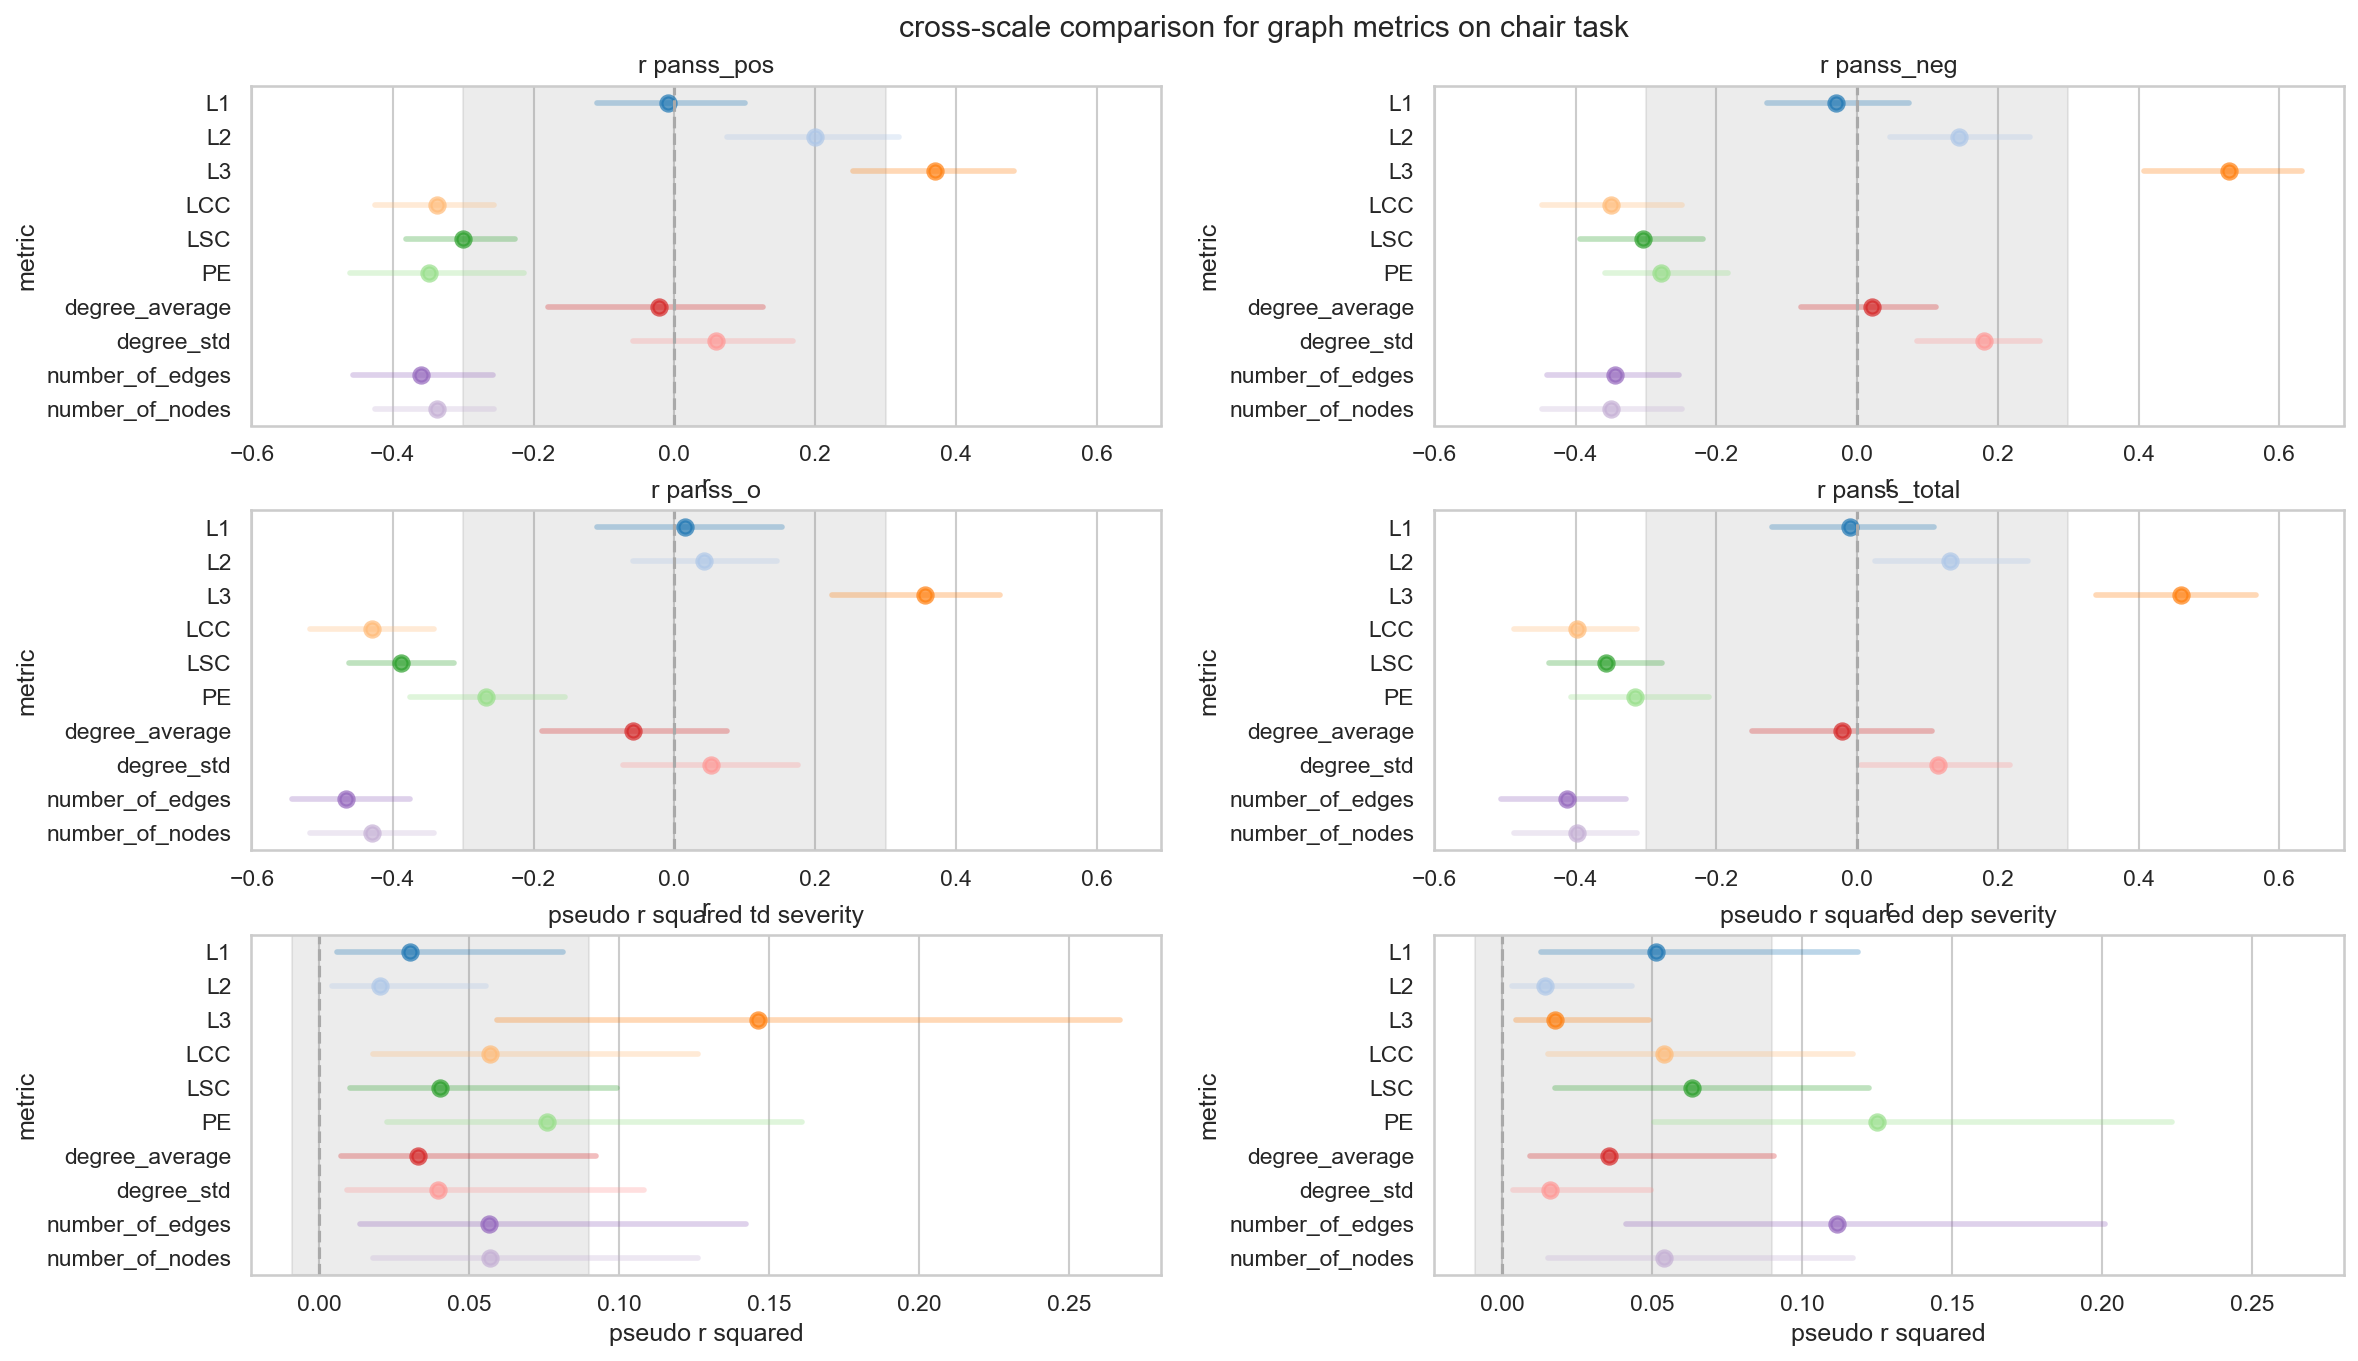
\includegraphics[width=1.1\textwidth, center]{Figures/chapter_4/graph/ru_chair_scale_r.png} 
\captionsetup{width=\textwidth}
\caption[Graph Metrics: Russian, Chair Task]{\label{fig:results:graph:ru:ch} Pearson's r correlation coefficient and pseudo r squared for each scale for the graph-based metrics on the Russian dataset, chair task. Grey indicates the values below the 0.3 threshold in absolute value or pseudo r squared below 0.09.}
\end{figure}

\clearpage
Figure \ref{fig:results:graph:ru:pr} shows the performance of graph-based metrics on present task. The largest connected and strongly connected component size as well as the number of nodes and edges correlated negatively with all PANSS scales and were also predictive of thought disorder severity. Additionally, on present task, average node degree and standard deviation in node degree correlated negatively with PANSS positive and total scores, and average degree was somewhat predictive of TD severity as well.  L1 correlated slightly with PANSS general score.

\begin{figure}[ht!]
    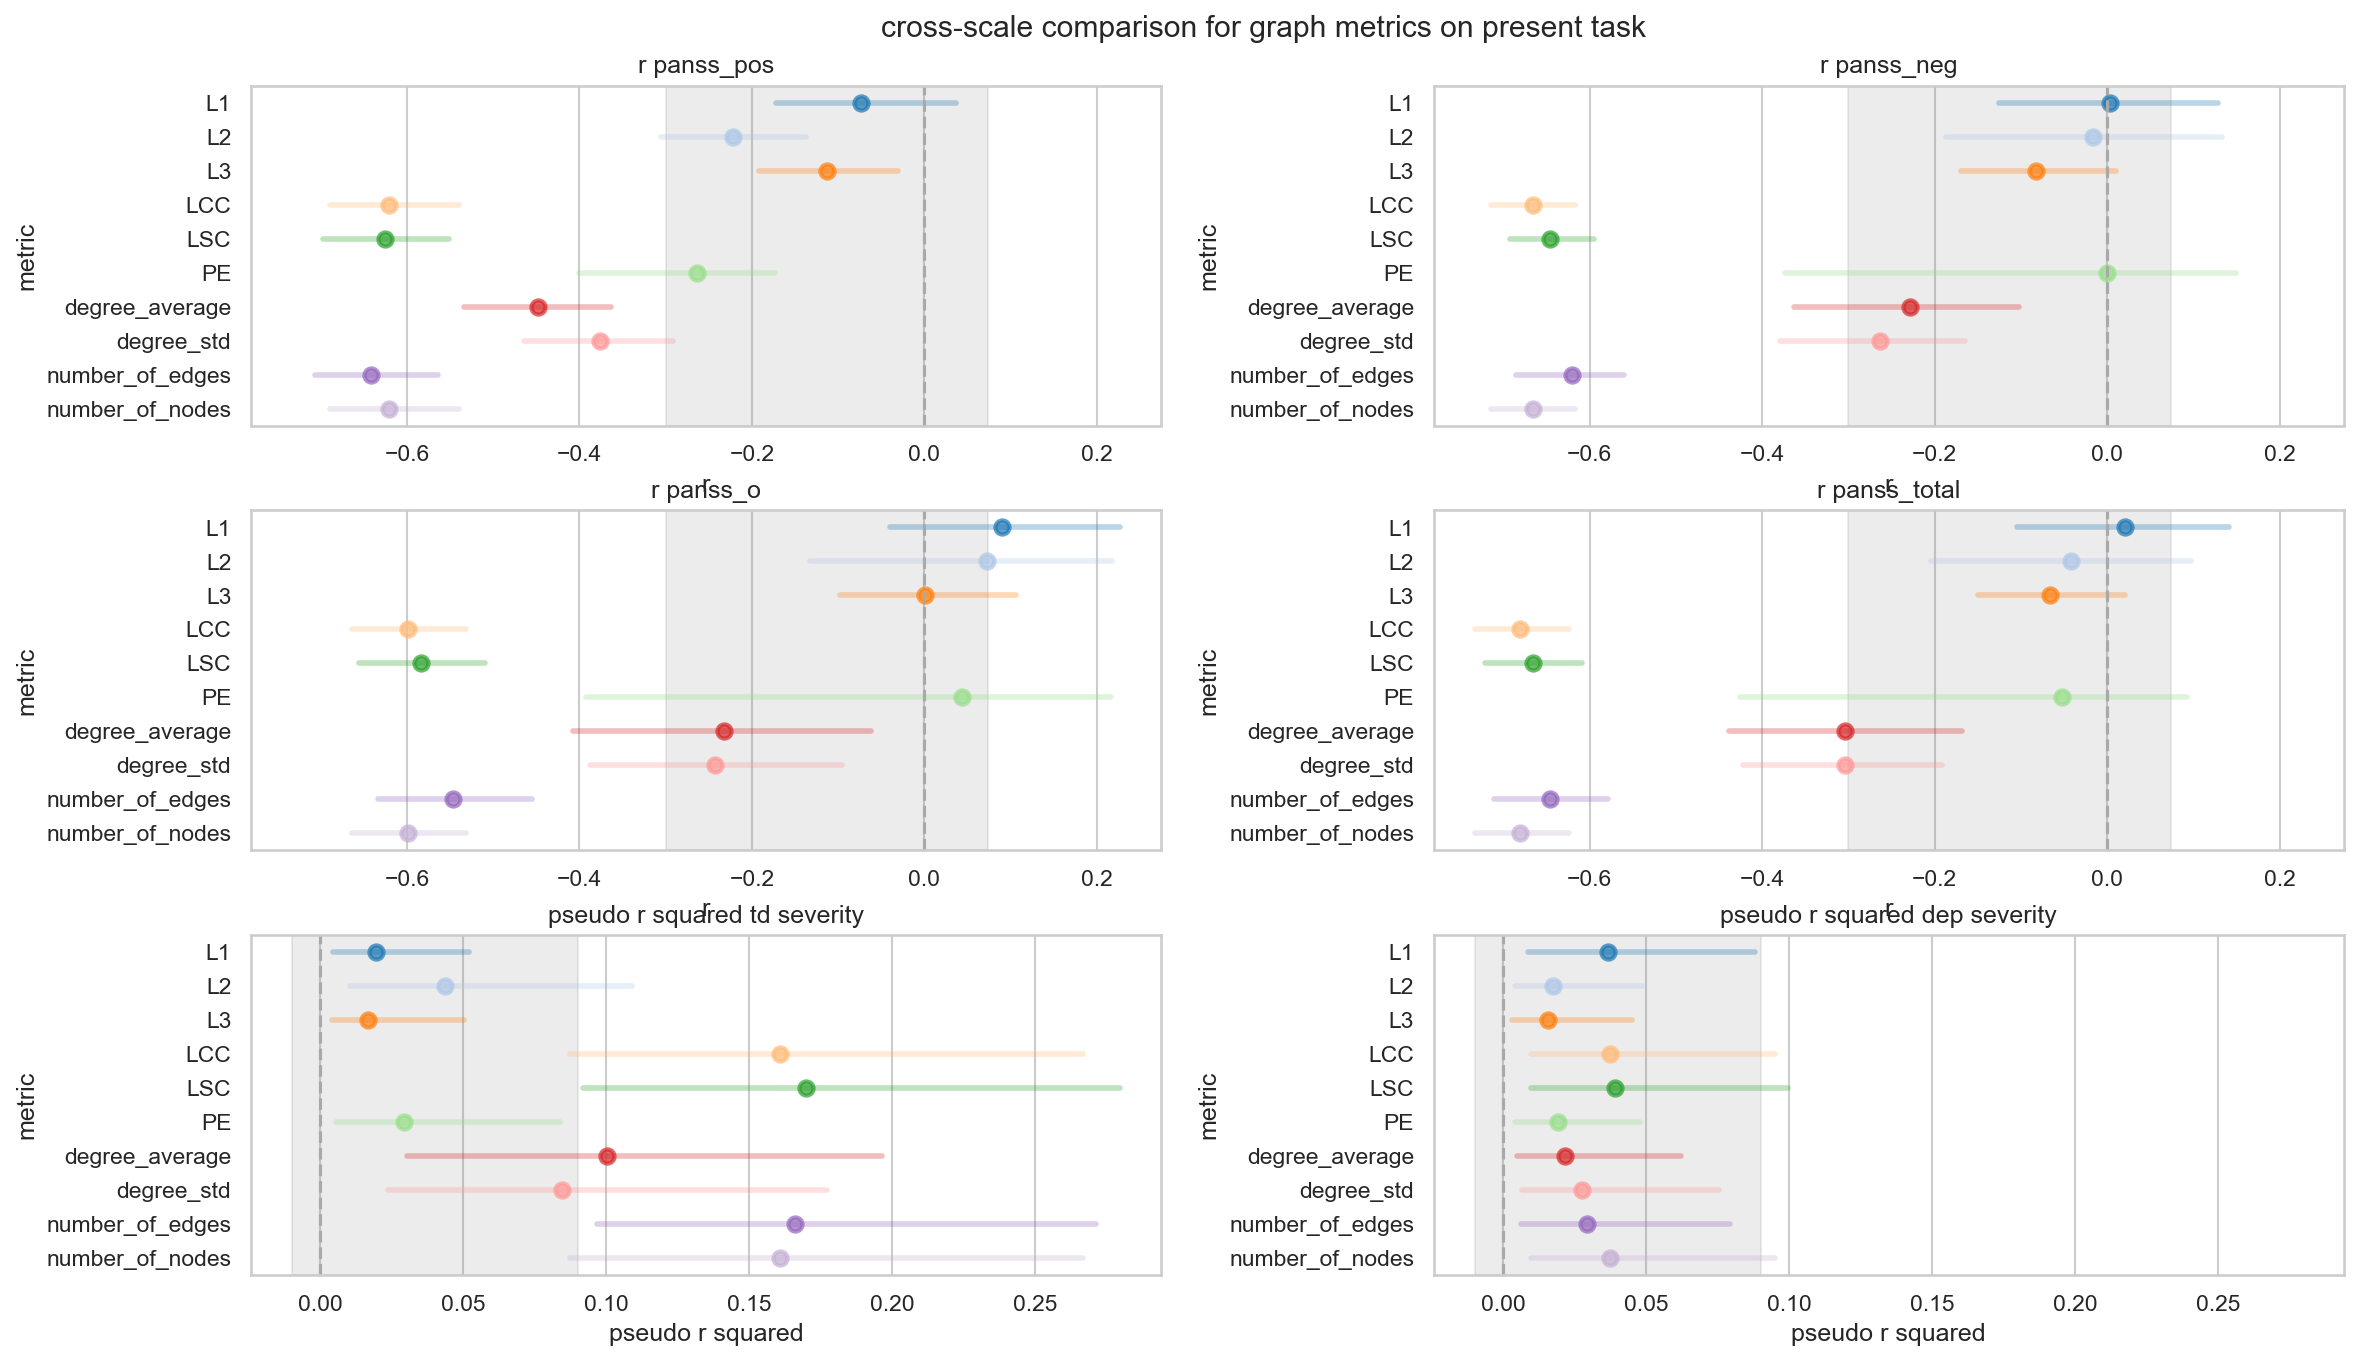
\includegraphics[width=1.1\textwidth, center]{Figures/chapter_4/graph/ru_present_scale_r.png} 
\captionsetup{width=\textwidth}
\caption[Graph Metrics: Russian, Present Task]{\label{fig:results:graph:ru:pr} Pearson's r correlation coefficient and pseudo r squared for each scale for the graph-based metrics on the Russian dataset, present task. Grey indicates the values below the 0.3 threshold in absolute value or pseudo r squared below 0.09.}
\end{figure}

Finally, figure \ref{fig:results:graph:ru:sp} shows the performance of graph-based metrics on sportsman task. As on other tasks, the largest connected and strongly connected component size as well as the number of nodes and edges correlated negatively with all PANSS scales. The number of parallel edges correlated negatively with all PANSS subscales but general and was also predictive of TD severity.

\begin{figure}[ht!]
    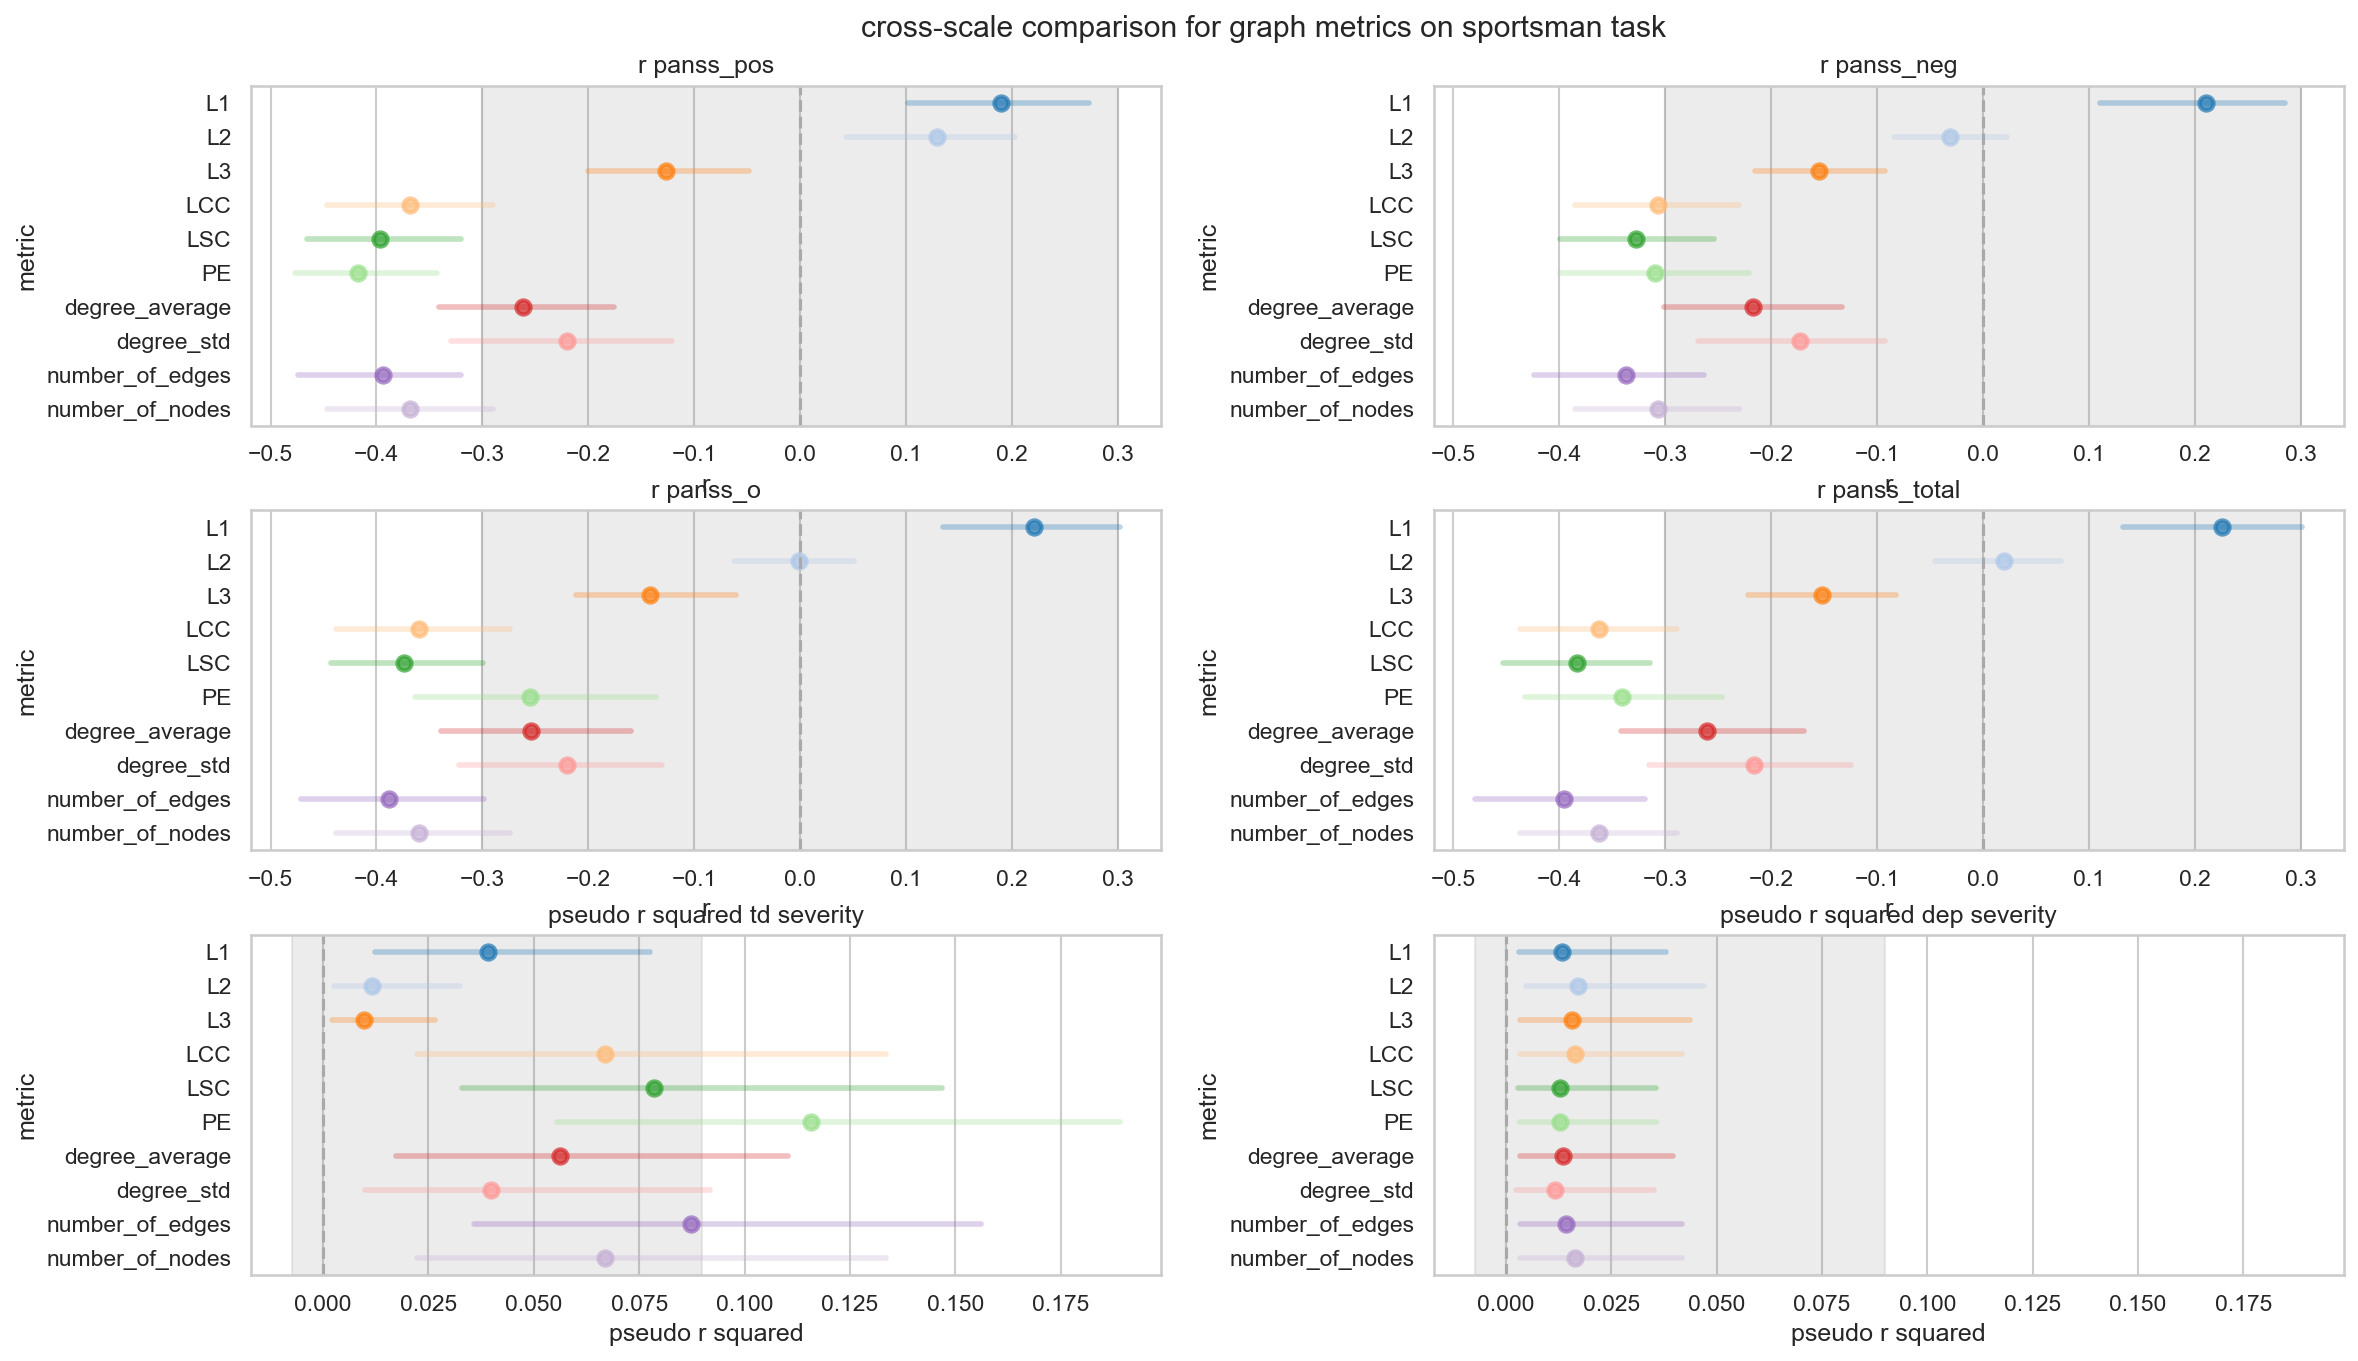
\includegraphics[width=1.1\textwidth, center]{Figures/chapter_4/graph/ru_sportsman_scale_r.png} 
\captionsetup{width=\textwidth}
\caption[Graph Metrics: Russian, Sportsman Task]{\label{fig:results:graph:ru:sp} Pearson's r correlation coefficient and pseudo r squared for each scale for the graph-based metrics on the Russian dataset, sportsman task. Grey indicates the values below the 0.3 threshold in absolute value or pseudo r squared below 0.09.}
\end{figure}


\begin{figure}[ht!]
    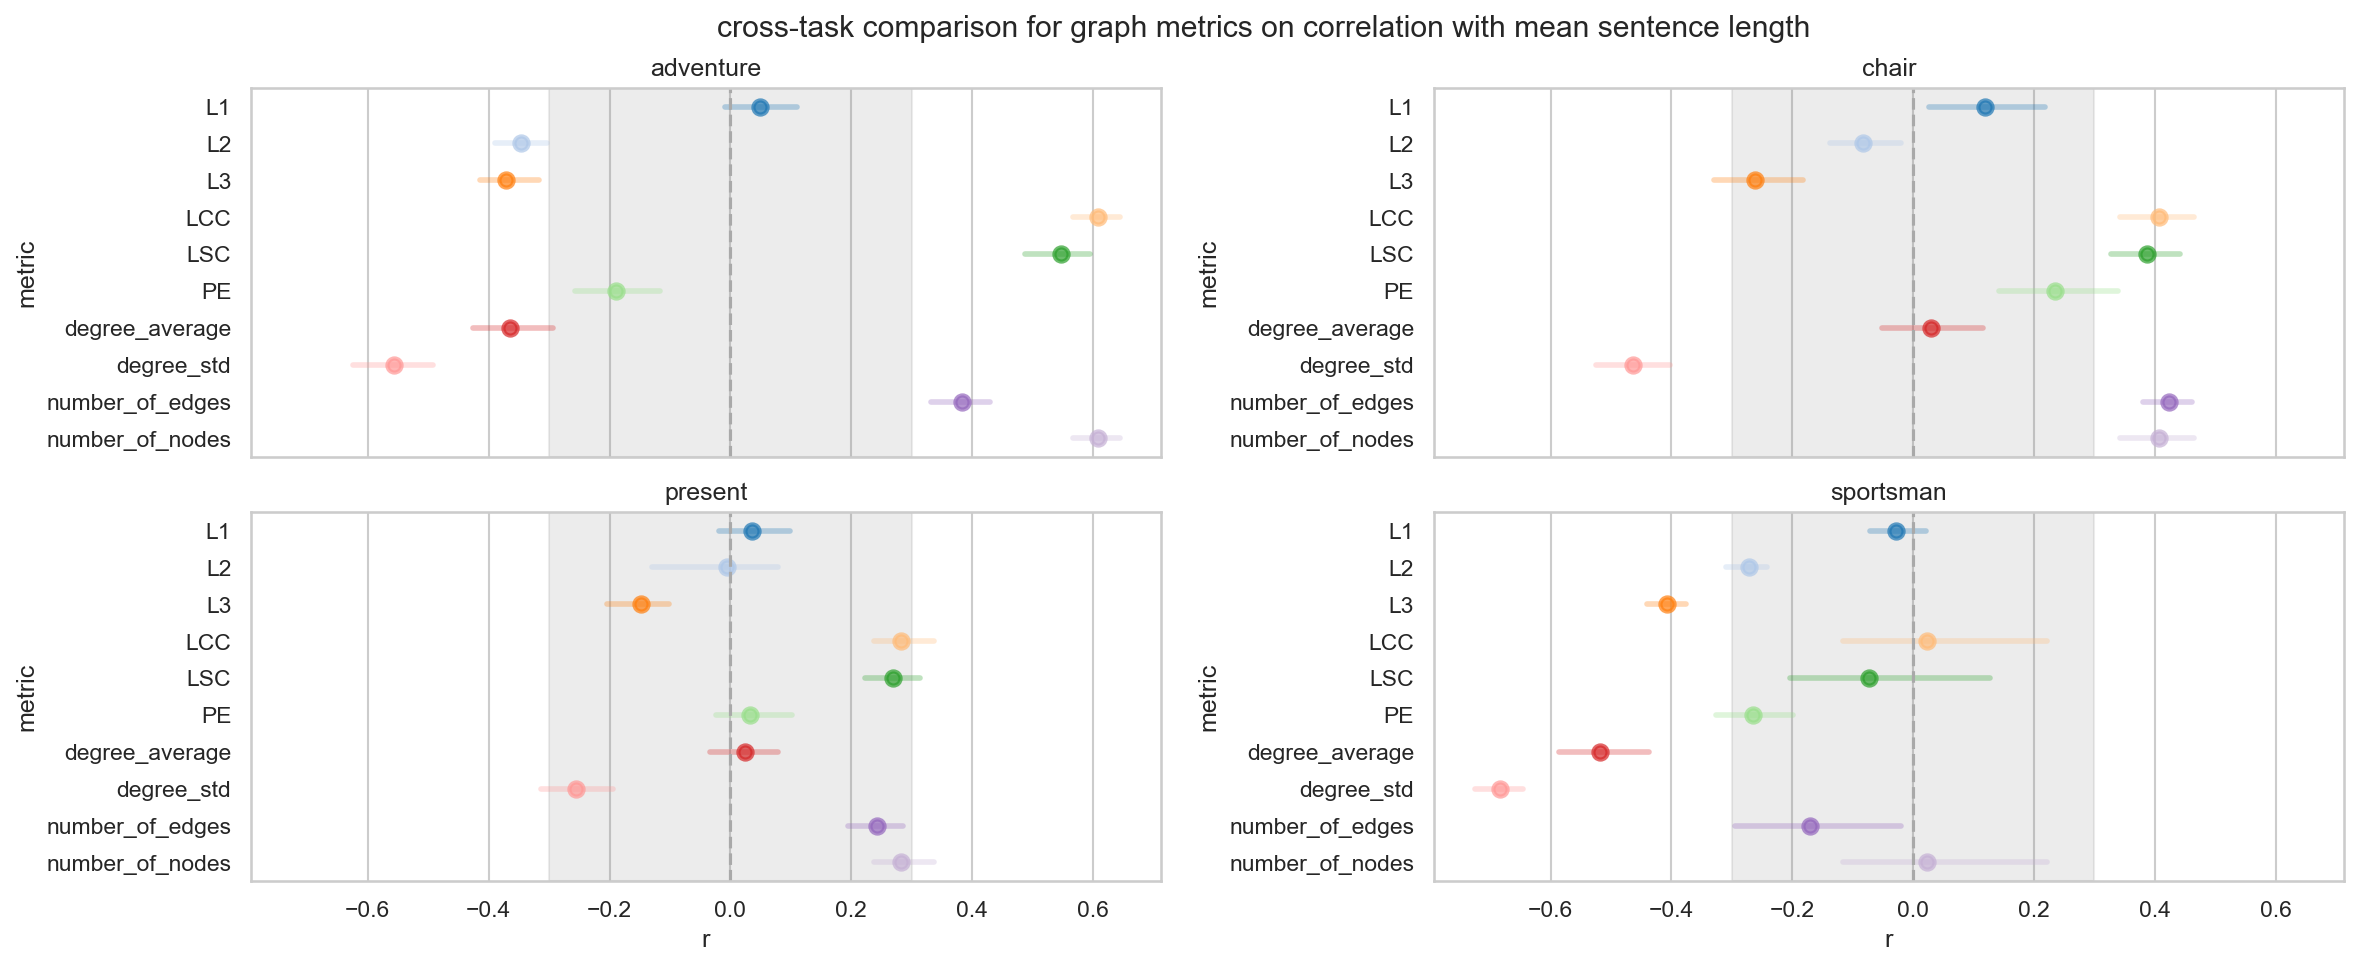
\includegraphics[width=1.1\textwidth, center]{Figures/chapter_4/graph/ru_corr_len.png} 
\captionsetup{width=\textwidth}
\caption[Syntactic Metrics: Russian, Length Correlation]{\label{fig:results:graph:ru:corr_len} Pearson's r correlation coefficient with mean sentence length for the graph-based metrics on the Russian dataset across tasks. Grey indicates the values below 0.3.}
\end{figure}

Figure \ref{fig:results:graph:ru:corr_len} shows the strength of correlation with mean sentence length across tasks. 
LCC, LSC, N, and E correlated positively with mean sentence length on adventure and chair tasks. L2 correlated negatively with mean sentence length on adventure task, and L3, average node degree, and standard deviation of node degree did so on adventure and sportsman tasks. The standard deviation of node degree also correlated negatively with mean sentence length on chair task.

Overall, among the graph-based metrics, LCC, LSC, N, and E showed the best performance on the Russian sample, as they correlated with some psychiatric scales across all of the tasks, though they also were correlated with mean sentence length on the two tasks where it could be expected, as they probably depended somewhat on the verbosity. The number of parallel edges performed on two of the four tasks, chair and sportsman, and the average and standard deviation in node degree, as well as loops of size one (lemma repetitions) and three, only performed on one task, namely, present.

\subsection{Cross-Linguistic Comparison}

Both on the German and Russian samples, LCC, LSC, N, and E were negatively correlated with negative and general symptoms scales and were also positively correlated with mean sentence length, though on the Russian sample, this correlation was present only for some tasks. As positive symptoms were more pronounced in the Russian sample, the same metrics were also correlated negatively with PANSS positive scale and on some tasks predictive of TD and depression severity. L1, L3, PE, average node degree, and standard deviation in node degree, were only correlated with symptom scales on the Russian sample.

%-----------------------------------
%	section 7
%-----------------------------------
\clearpage
\section{Language Model-Based Methods}
\label{sec:results:clinical:LM}

This section covers the results of the language model-based metrics for both languages. The metrics included cumulative global coherence (\texttt{cgcoh}), global coherence (\texttt{gcoh}), local coherence (\texttt{lcoh}), second order coherence (\texttt{scoh}), next sentence probability (\texttt{sprob}), and pseudo-perplexity (\texttt{pppl}). The models included BERT and two weighting schemes for word2vec. \texttt{BERT} is denoted as such, \texttt{w2v} stands for word2vec (fasttext), \texttt{glove} stands for GloVe, and \texttt{tf} on figures stands for TF-IDF weighted sentence scheme, while \texttt{avg} for simple sentence averaging. 

\subsection{German}

Figure \ref{fig:results:lm:de} shows the performance of Language Model-based metrics on the German sample.

\begin{figure}[h!]
    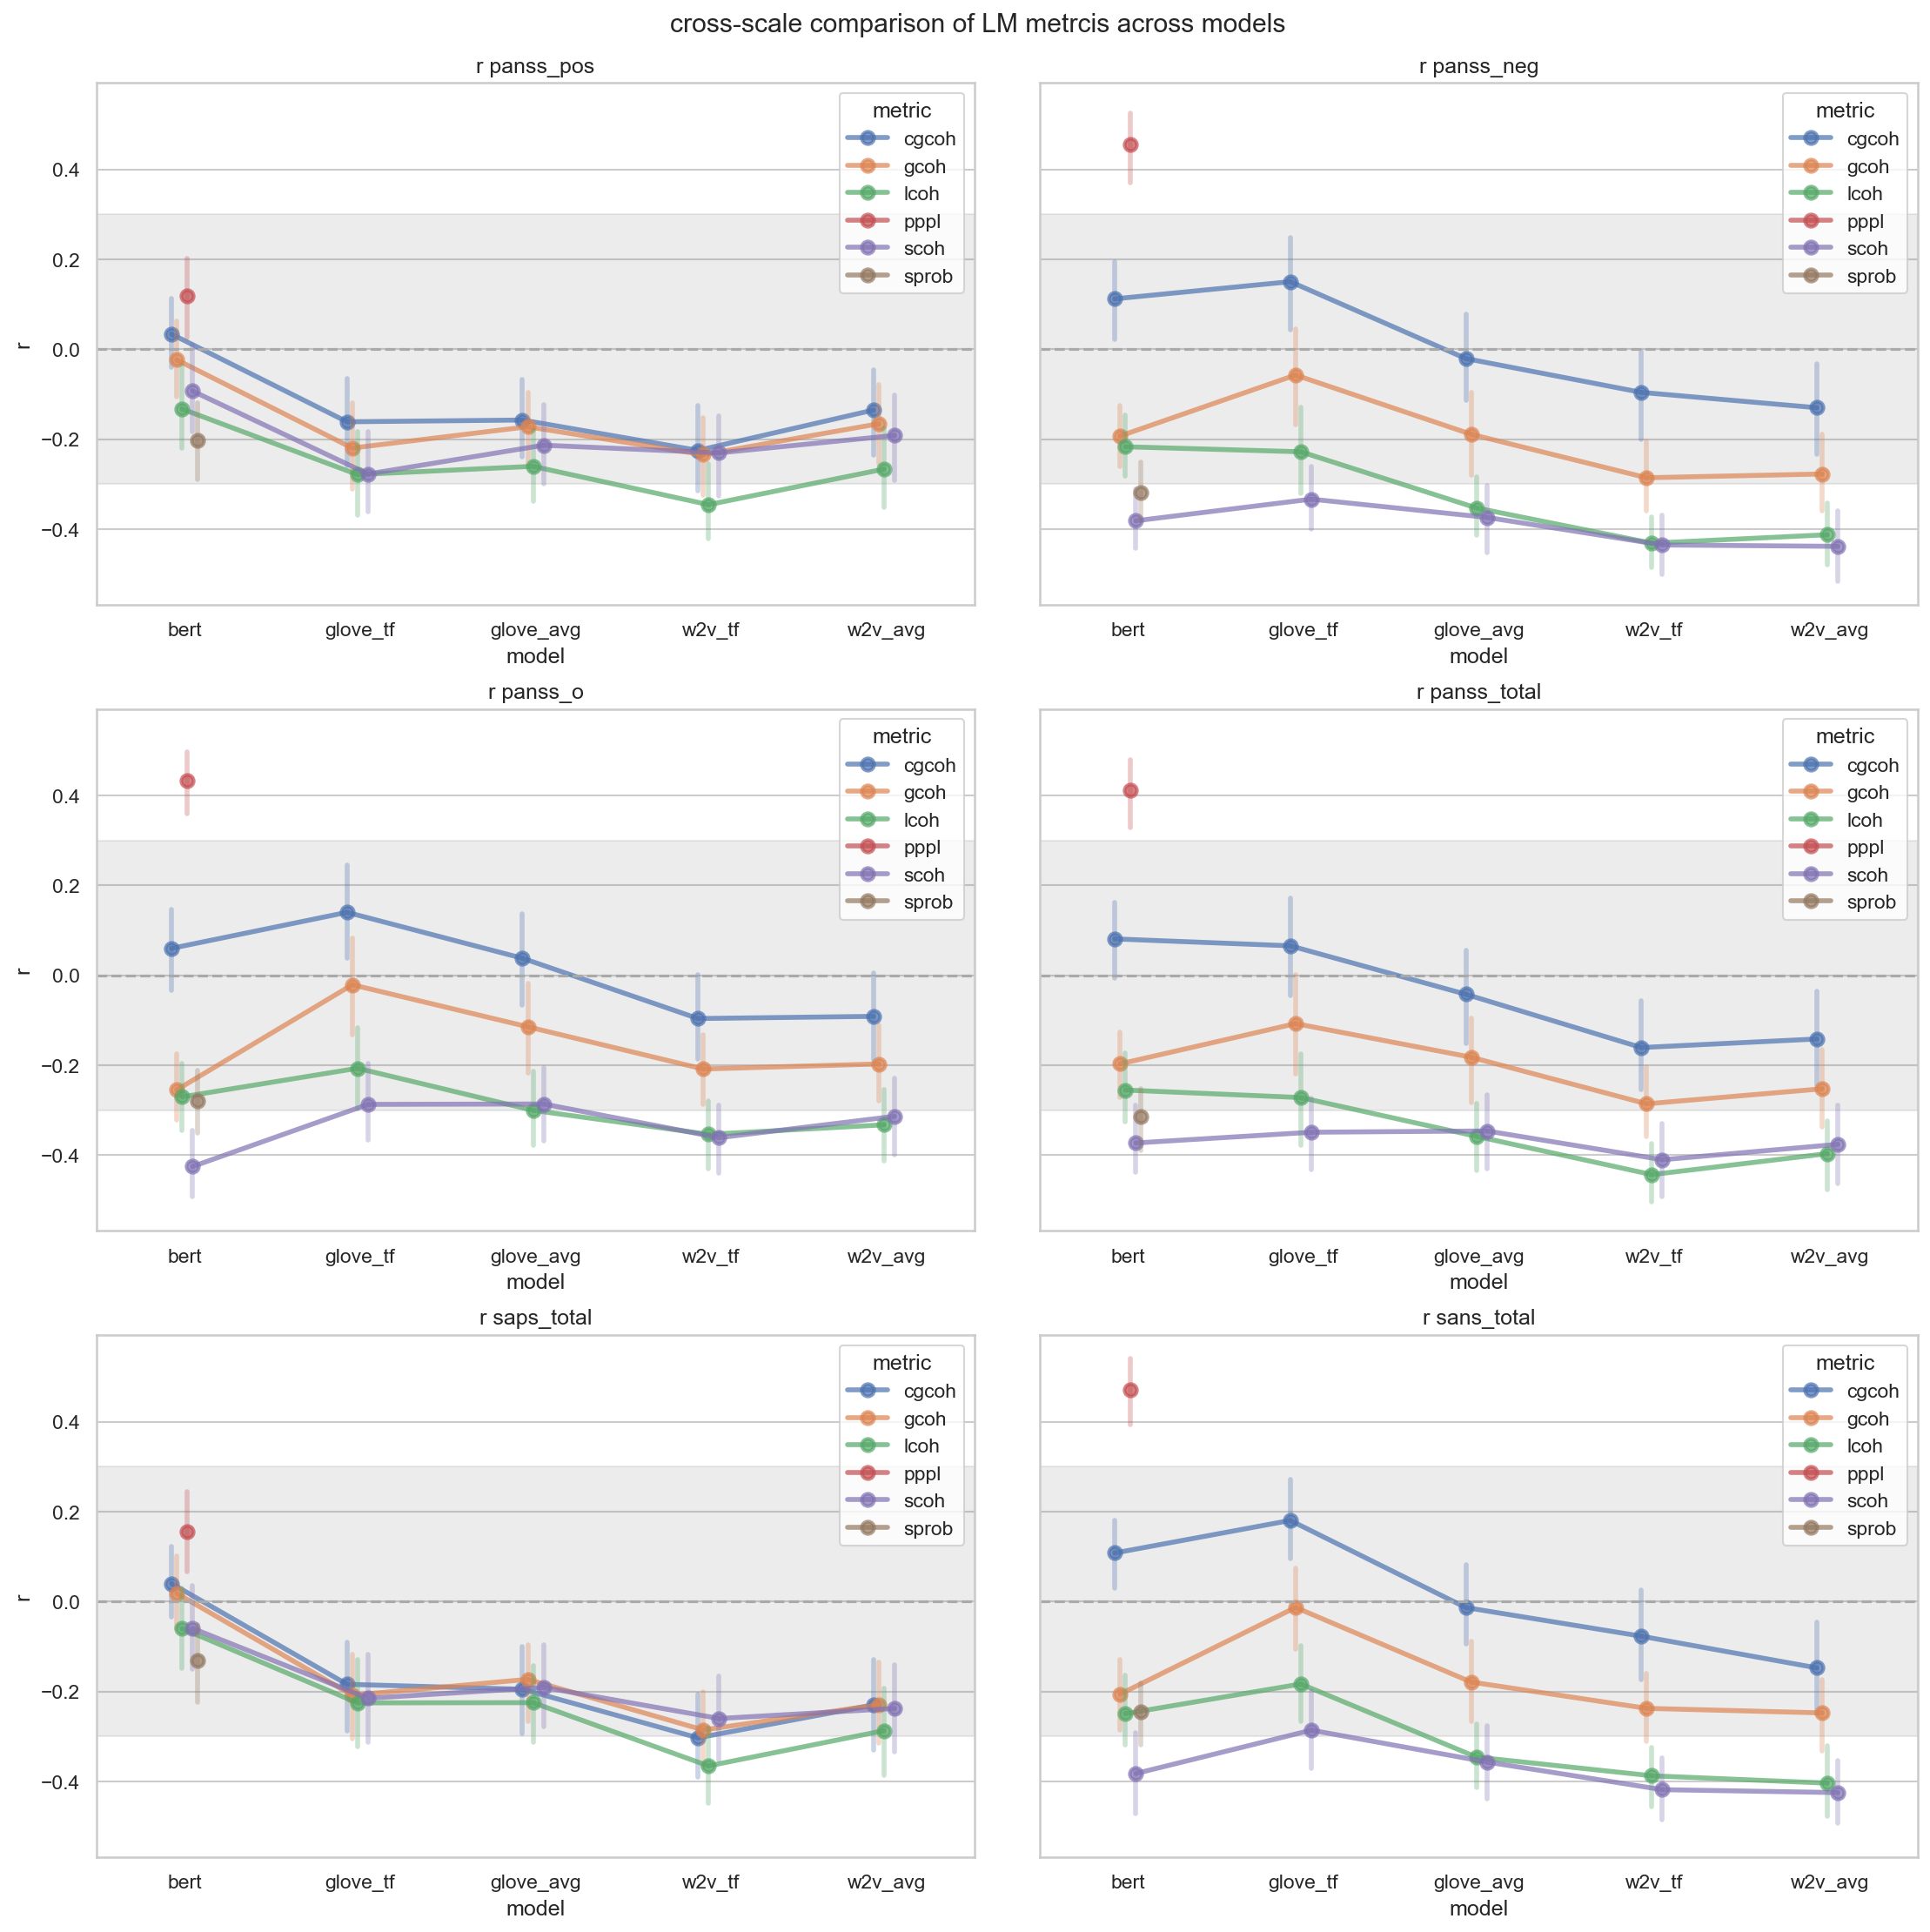
\includegraphics[width=1.1\textwidth, center]{Figures/chapter_4/LM/de_scale_r.png} 
\captionsetup{width=\textwidth}
\caption[LM Metrics: German]{\label{fig:results:lm:de} Pearson's r correlation coefficient with each scale for the LM-based metrics on the German dataset. Grey indicates the values below the 0.3 threshold in absolute value.}
\end{figure}

% hierarchy of metrics
Overall, there was a hierarchy of metrics, with pseudo-perplexity performing the best, positively correlating with negative and general symptom severity. The second-best performing metric was second-order coherence, which correlated negatively across models with negative symptoms and total PANSS, and on all models but averaged GloVe with general PANSS. Local coherence and next sentence probability showed similar levels of performance, with local coherence correlating stronger on word2vec and averaged GloVe, but not BERT, TF-IDF weighted word2vec even correlating negatively with positive symptom severity. Next sentence probability only reached the threshold in negative correlation with PANSS negative and total. Finally, global and cumulative global coherence performed the worst and did not correlate strongly with any of the scales.
% cgcoh    0.120598
% gcoh     0.181313
% sprob    0.248705
% lcoh     0.295024
% scoh     0.311049
% pppl     0.340907

% hierarchy of models
As for the models, on the cosine similarity-based metrics, word2vec showed the best performance with TF-IDF averaging followed by simple averaging, and GloVe, where the pattern was reversed, simple averaging outperforming TF-IDF. For both models, the difference between the averaging schemes was slight. Finally, BERT performed worst for the cosine similarity-based metrics, but the two feature-based metrics performed relatively well.
% bert         0.176137
% glove_tf     0.193866
% glove_avg    0.212054
% w2v_avg      0.263709
% w2v_tf       0.289213

% glove_tf     0.193866
% glove_avg    0.212054
% bert         0.215694
% w2v_avg      0.263709
% w2v_tf       0.289213

Figure \ref{fig:results:lm:de:ttest} shows the results of a bidirectional t-test against the strength of correlation with mean sentence length. Except for pseudo-perplexity, which was somewhat lower in patients than in controls, no metric could differentiate between the groups.

\begin{figure}[ht!]
    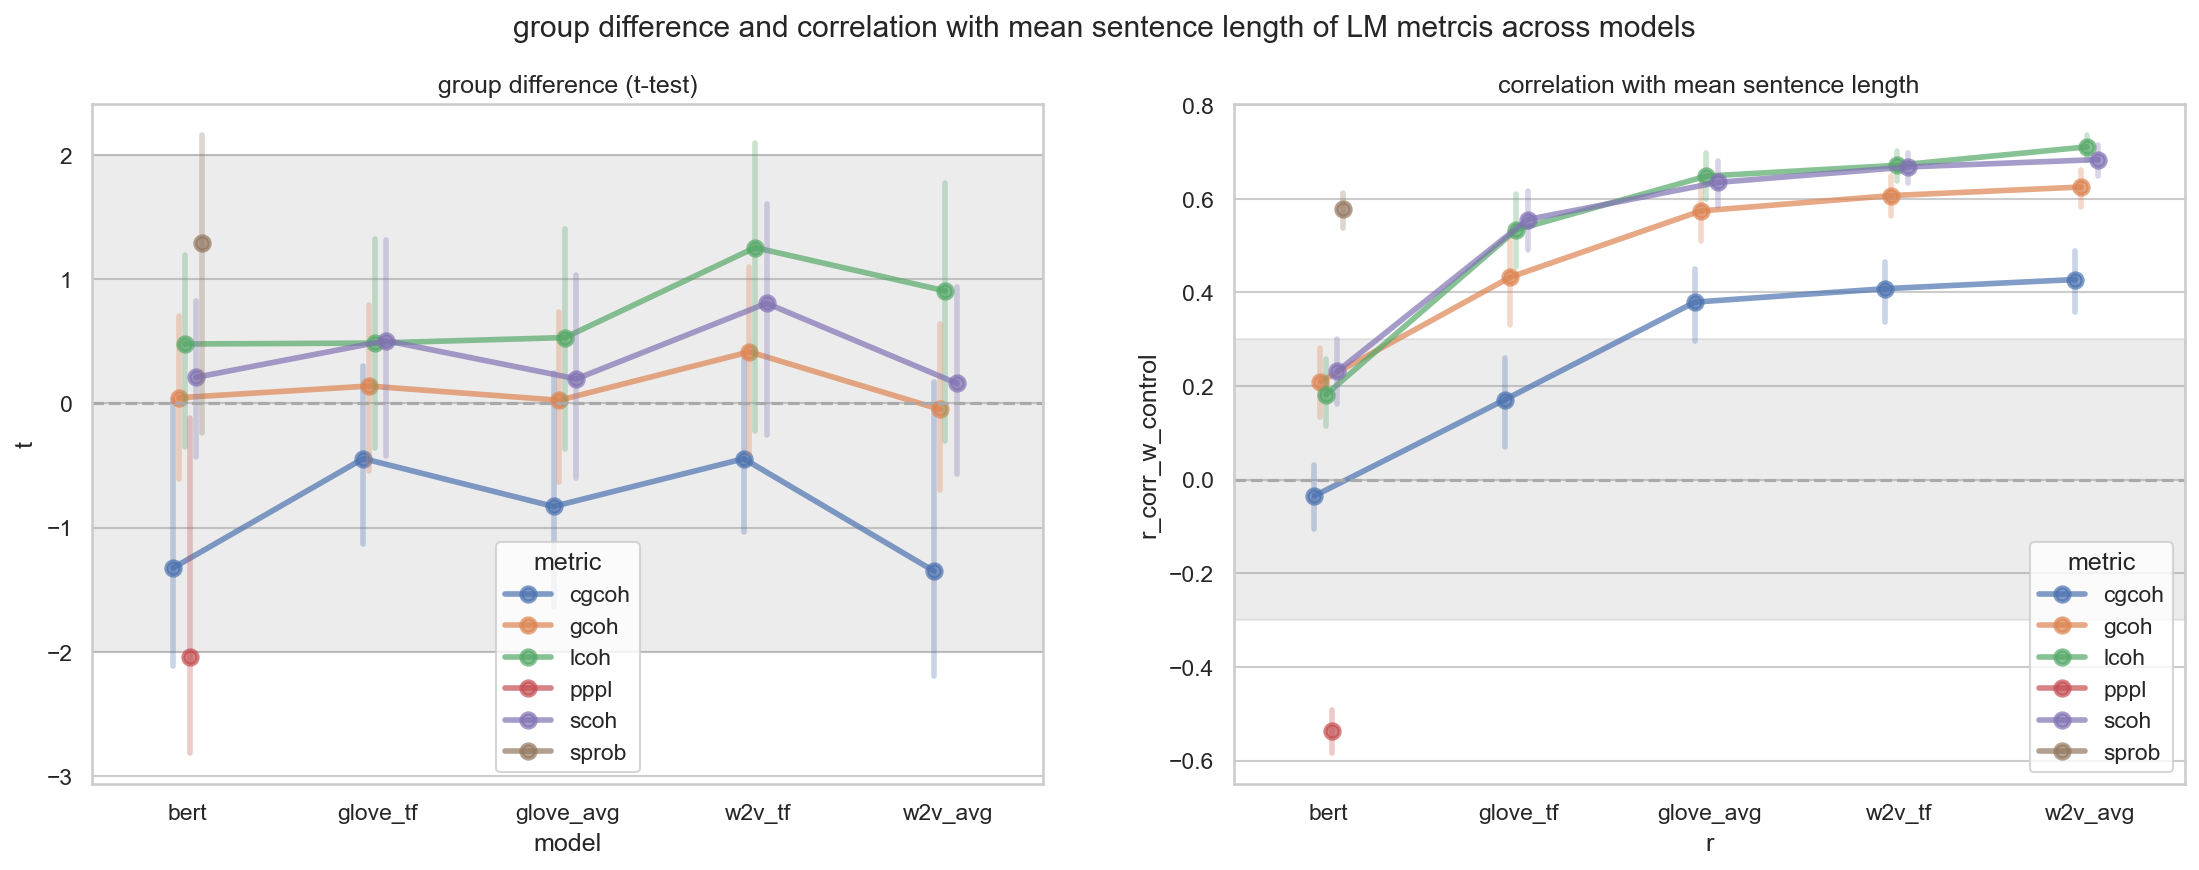
\includegraphics[width=1.1\textwidth, center]{Figures/chapter_4/LM/de_t_test_corr_len.png} 
\captionsetup{width=\textwidth}
\caption[LM Metrics: German (T-Test)]{\label{fig:results:lm:de:ttest} T-test and Pearson's r correlation coefficient with mean sentence length for the LM-based metrics on the German dataset. Grey indicates the values below 2 for t score and below the 0.3 threshold in absolute value for correlation coefficient.}
\end{figure}

% corr len
The cumulative global coherence was least correlated with mean sentence length, followed by global coherence, and then all other metrics. Interestingly, both next sentence probability and pseudo-perplexity were strongly correlated with mean sentence length, though the former was correlated positively and the latter negatively. For the cosine similarity-based metrics, BERT was uncorrelated with mean sentence length. GloVe-based metrics were less correlated than w2v, and the TF-IDF weighted metrics were somewhat less correlated than simple averaged ones. There was an inverse relation trend between overall metric performance and its correlation with mean sentence length, being more pronounced for the correlation with symptom scales, than for the T-test results.

There was an interesting pattern, that cumulative global coherence tended to correlate less negatively (and, in some cases, more positively) than other metrics, and it was followed by global coherence, while local and second-order coherence tended to correlate more negatively with symptom severity.

\subsection{Russian}
Out of the four tasks, on one no LM metric correlated with any of the psychiatric scales, while on the other three, there was some predictive power.

\clearpage
Figure \ref{fig:results:lm:ru:ad} shows the comparative LM-based metric performance across scales, metrics, and models on adventure task.

\begin{figure}[ht!]
    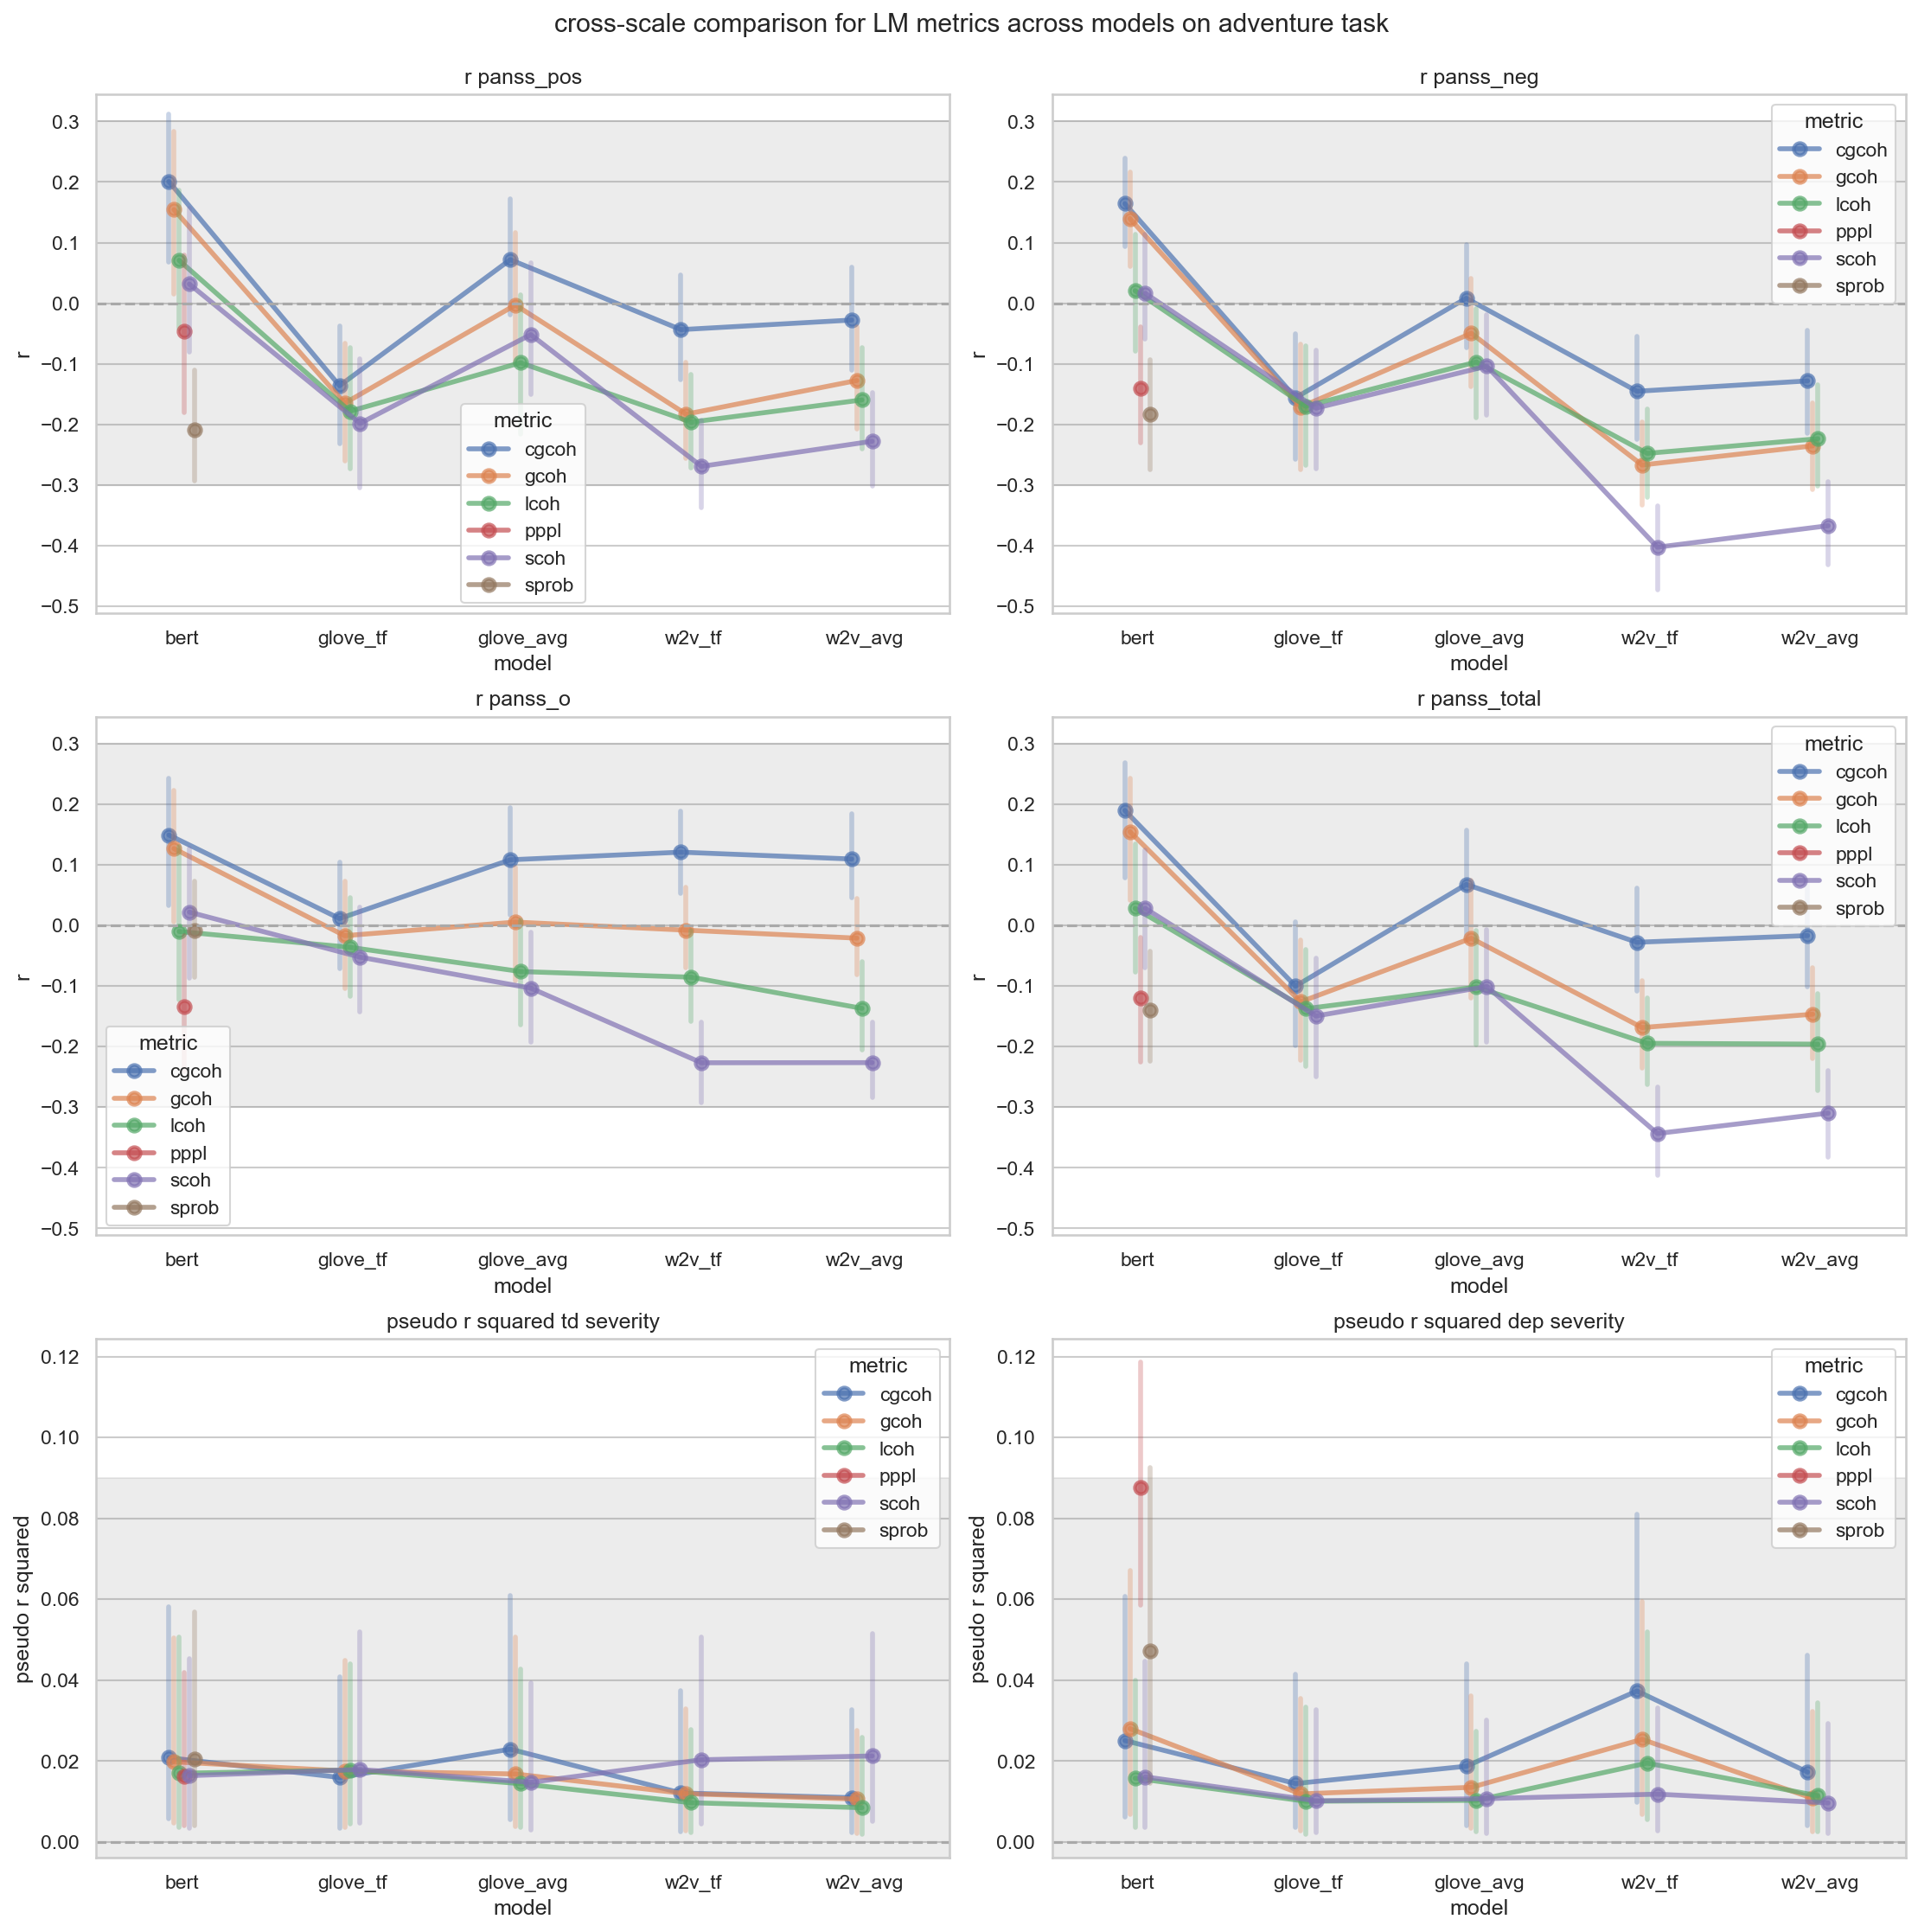
\includegraphics[width=1.1\textwidth, center]{Figures/chapter_4/LM/ru_adventure_scale_r.png} 
\captionsetup{width=\textwidth}
\caption[LM Metrics: Russian, Adventure Task]{\label{fig:results:lm:ru:ad} Pearson's r correlation coefficient and pseudo r squared for each scale for the language model-based metrics on the Russian dataset, adventure task. Grey indicates the values below the 0.3 threshold in absolute value or pseudo r squared below 0.09.}
\end{figure}

% hierarchy of metrics
There was only one metric, that interacted with any scales, namely, second-order coherence, which correlated negatively with PANSS negative and total when calculated with either word2vec weighting scheme. For other metrics, even tough they did not reach the threshold, there was a hierarchy in performance, with second-order coherence being followed by next sentence probability and pseudo-perplexity, and then by local coherence and the two global coherence metrics. 
% cgcoh    0.112622
% gcoh     0.119337
% lcoh     0.120814
% pppl     0.144064
% sprob    0.150057
% scoh     0.153954


% hierarchy of models
word2vec, on average, seemed to outperform the other models, with TF-IDF averaging improving the performance compared to simple averaging for both word2vec and GloVe. BERT under-performed on this task, except for the feature-based metrics. Cosine similarity-based metrics calculated using BERT embeddings, unlike those calculated with either non-contextualized embedding model, tended to correlate positively, rather than negatively, with symptom severity.
% glove_avg    0.085626
% bert         0.109769
% glove_tf     0.122346
% w2v_avg      0.148203
% w2v_tf       0.167033


Figure \ref{fig:results:lm:ru:ch} shows the comparative LM-based metric performance across scales, metrics, and models on chair task. 

Only on this task, depression severity could be predicted, and GloVe TF-IDF could predict depression severity with all metrics but cumulative global coherence. Additionally, averaged word2vec cumulative global coherence correlated positively with general symptoms. 

% hierarchy of metrics
Generally, on this task cumulative global coherence correlated most strongly with symptom severity, followed by pseudo-perplexity, while local coherence and second-order coherence performed worse, and the next sentence prediction showed the worst performance. 
% sprob    0.085901
% lcoh     0.118644
% scoh     0.126696
% gcoh     0.138578
% pppl     0.160010
% cgcoh    0.190945

% hierarchy of models
Among the models, there was no clear patter on this task, though GloVe outperformed word2vec, and TF-IDF outperformed simple averaging, with BERT showing middle correlation strength.
% w2v_avg      0.129196
% glove_avg    0.133443
% bert         0.137969
% w2v_tf       0.140056
% glove_tf     0.167498


\begin{figure}[ht!]
    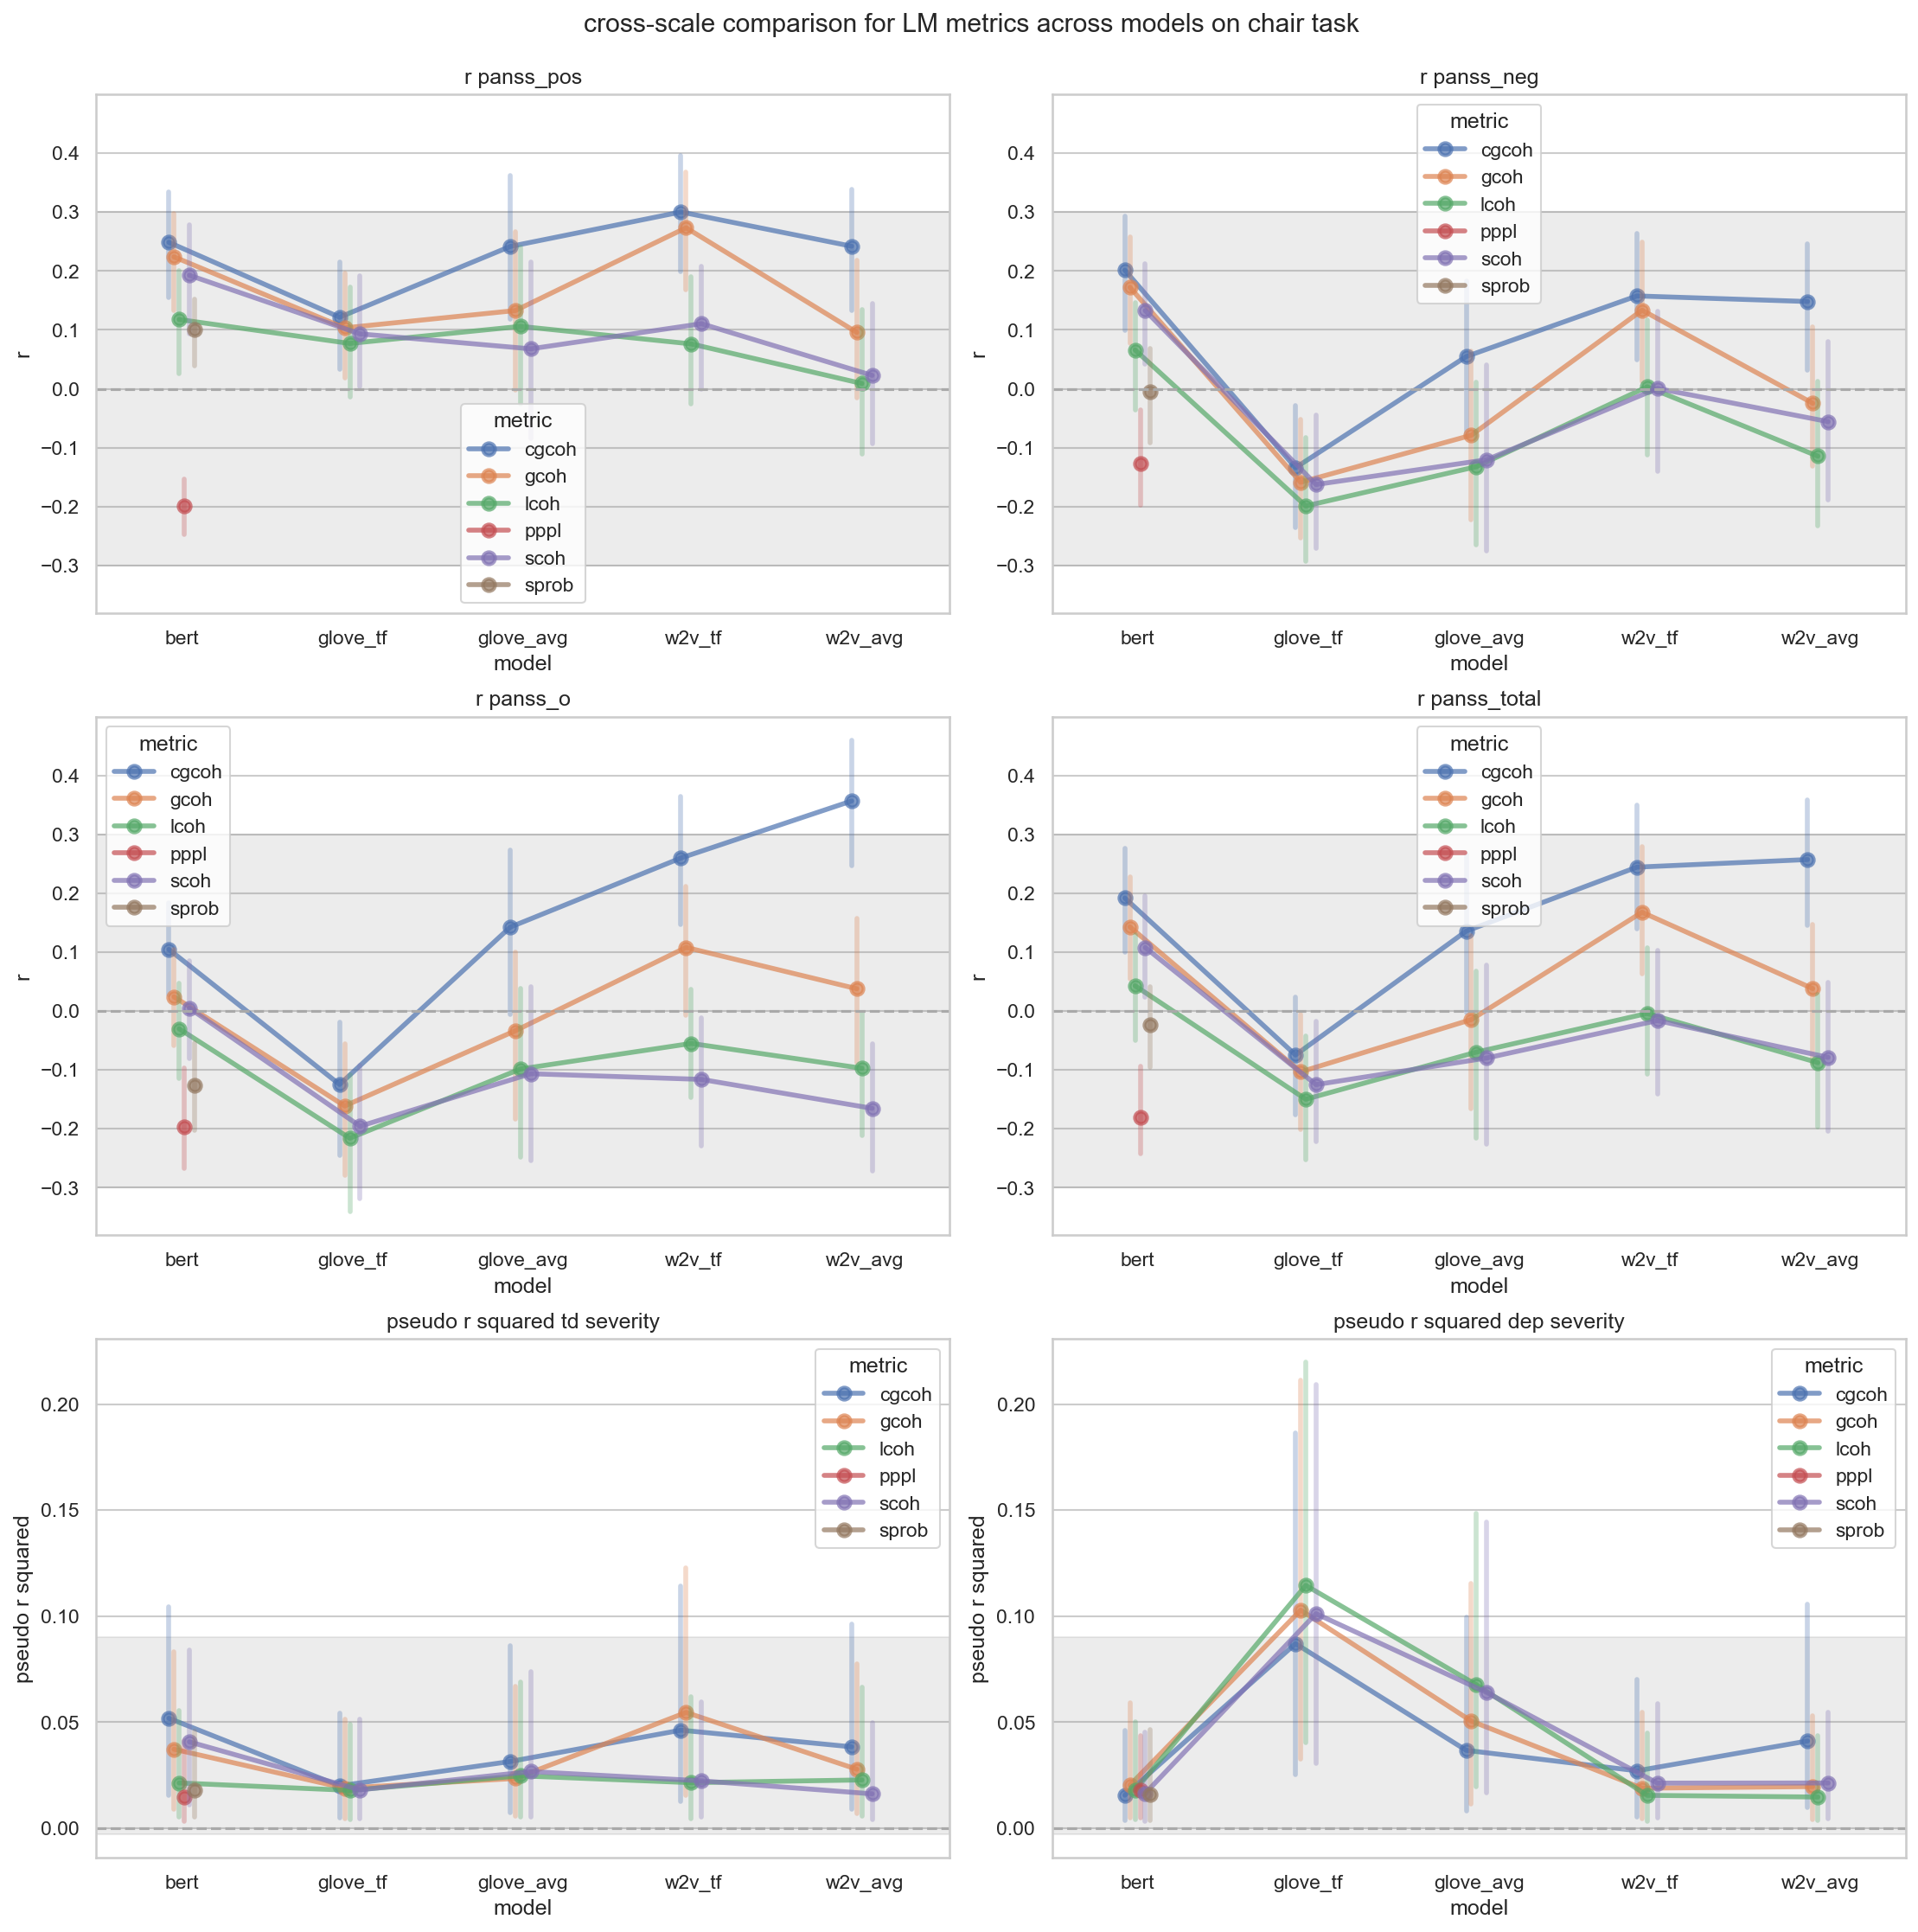
\includegraphics[width=1.1\textwidth, center]{Figures/chapter_4/LM/ru_chair_scale_r.png} 
\captionsetup{width=\textwidth}
\caption[LM Metrics: Russian, Chair Task]{\label{fig:results:lm:ru:ch} Pearson's r correlation coefficient and pseudo r squared for each scale for the language model-based metrics on the Russian dataset, chair task. Grey indicates the values below the 0.3 threshold in absolute value or pseudo r squared below 0.09.}
\end{figure}

\clearpage
Figure \ref{fig:results:lm:ru:pr} shows the comparative LM-based metric performance across scales, metrics, and models on present task. 

\begin{figure}[ht!]
    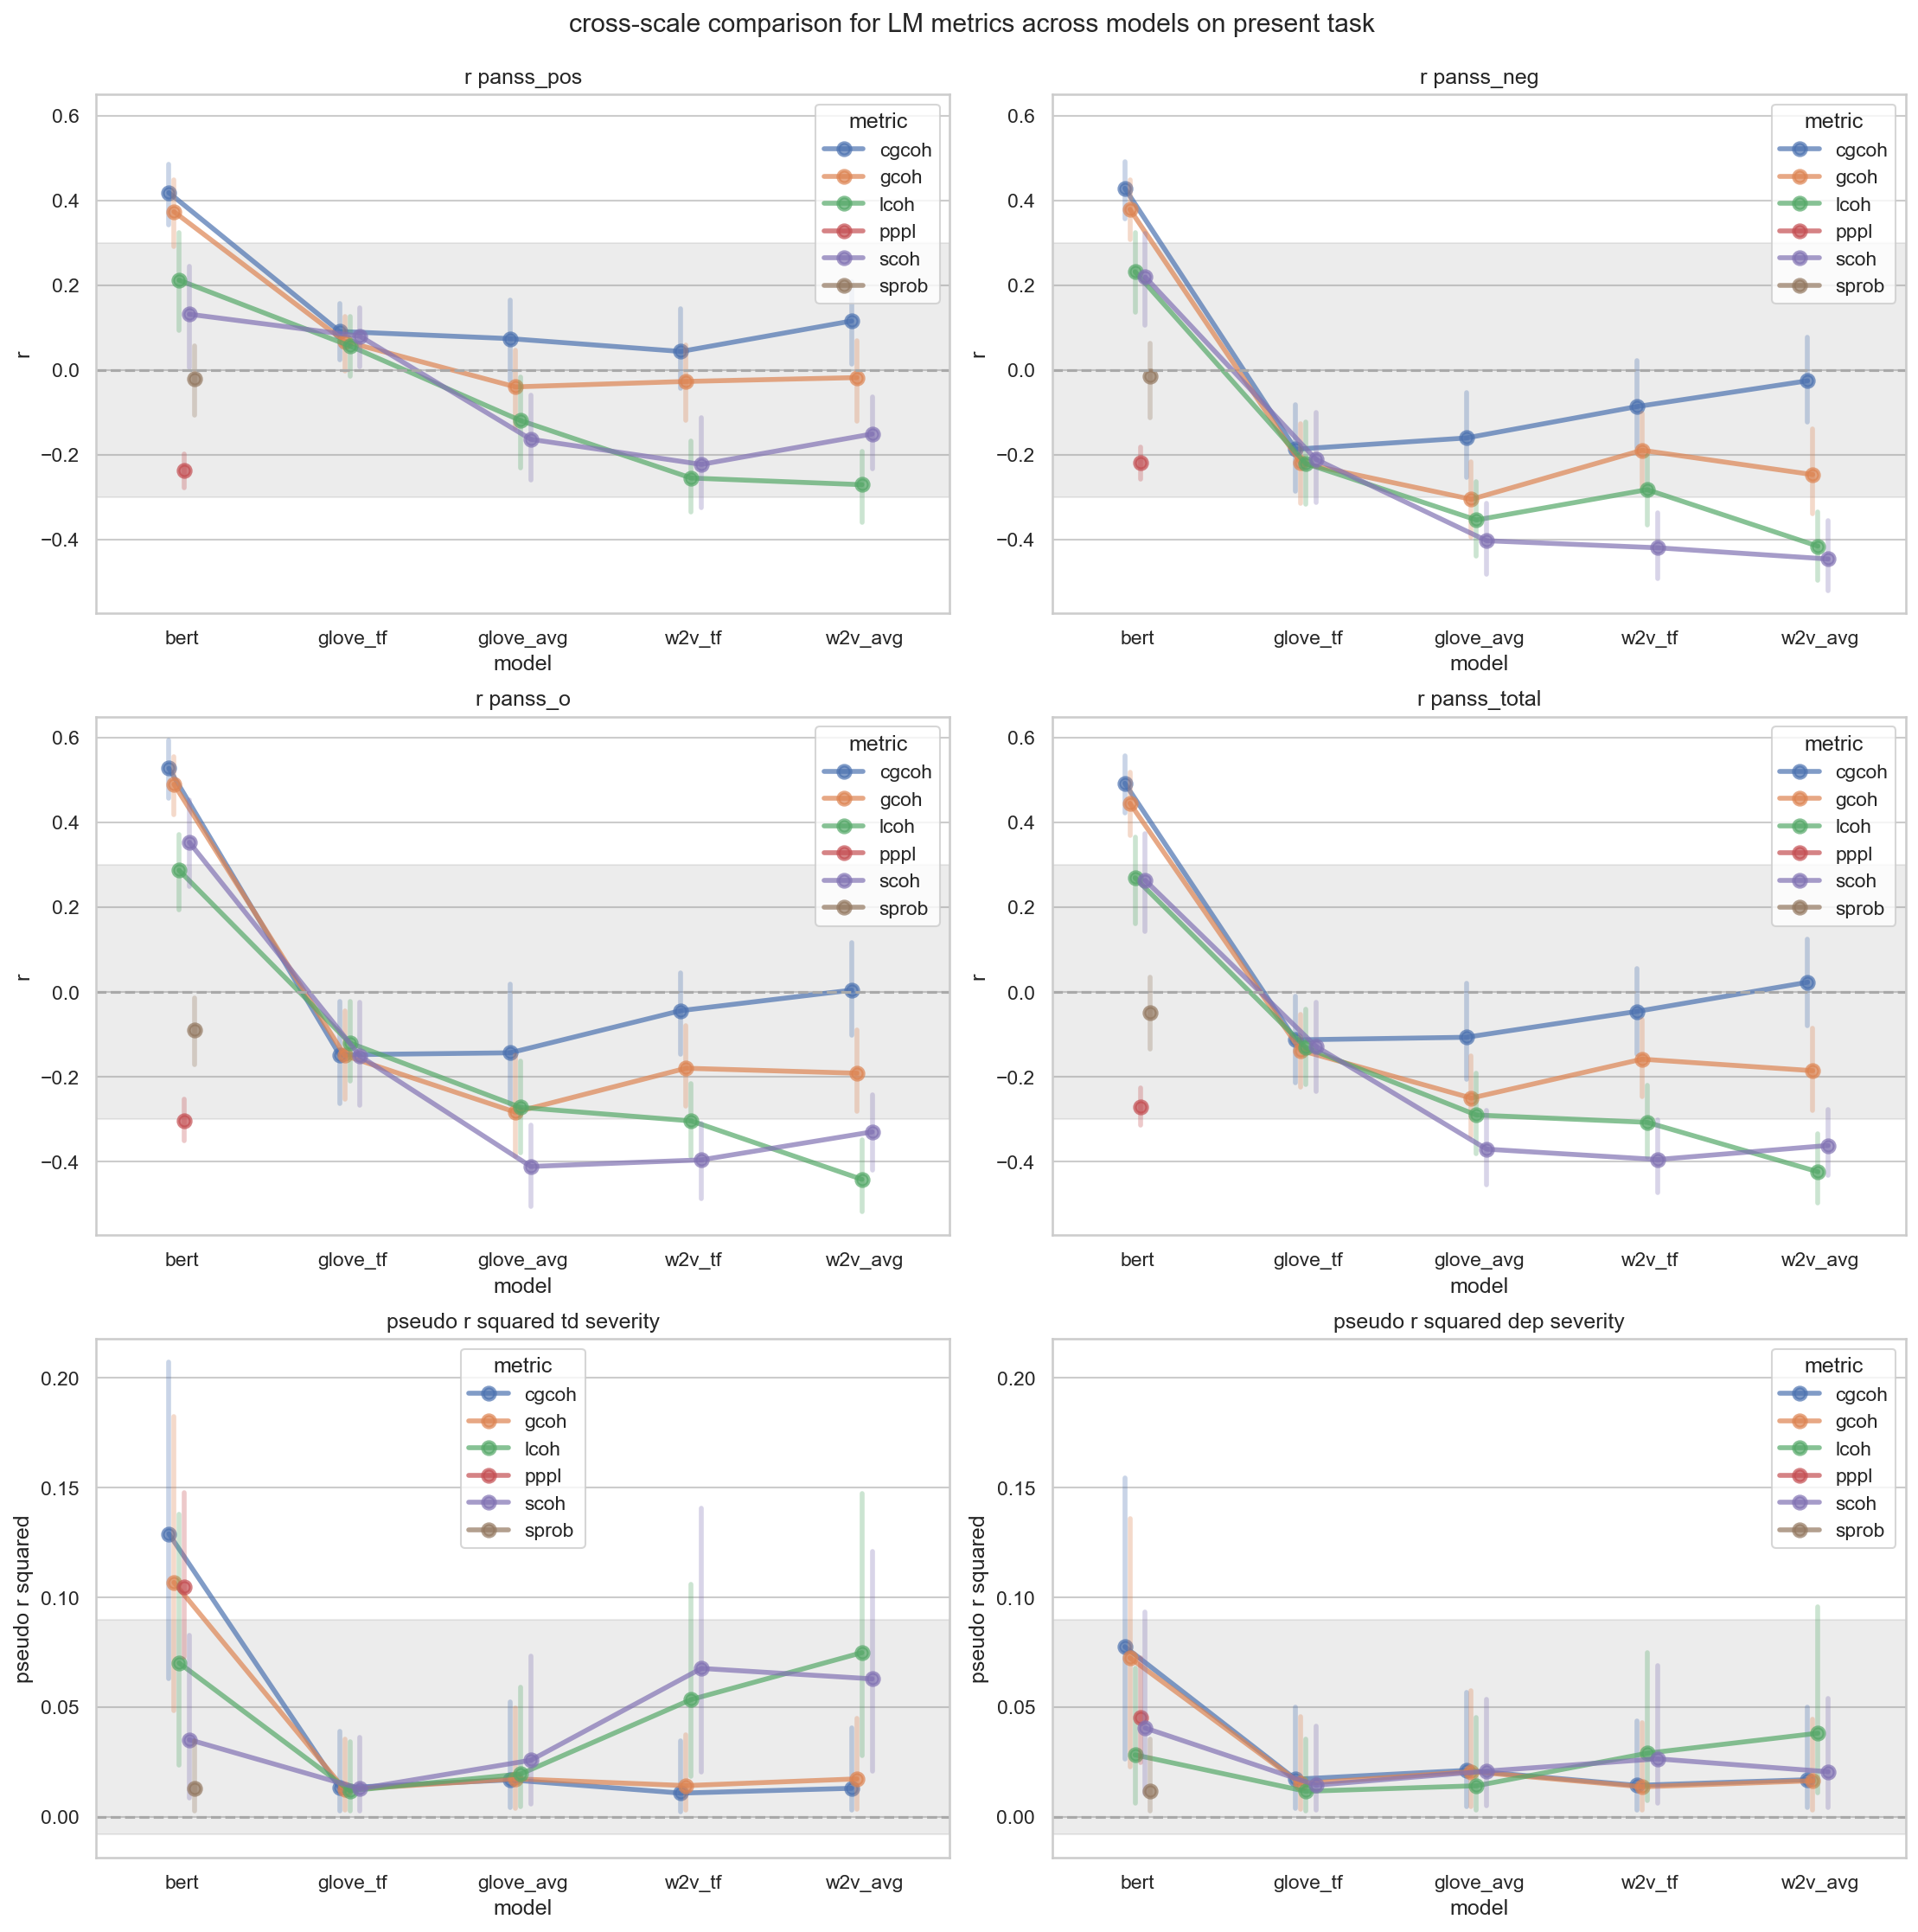
\includegraphics[width=1.1\textwidth, center]{Figures/chapter_4/LM/ru_present_scale_r.png} 
\captionsetup{width=\textwidth}
\caption[LM Metrics: Russian, Present Task]{\label{fig:results:lm:ru:pr} Pearson's r correlation coefficient and pseudo r squared for each scale for the language model-based metrics on the Russian dataset, present task. Grey indicates the values below the 0.3 threshold in absolute value or pseudo r squared below 0.09.}
\end{figure}

On present task, BERT global and cumulative global coherence correlated positively with all scales, while pseudo-perplexity correlated negatively with general symptoms, and they were all predictive of TD severity. Second-order coherence calculated using word2vec with either averaging or GloVe with simple averaging correlated negatively with all PANSS subscales but positive. Local coherence calculated using word2vec correlated negatively with PANSS general and total scores, and when calculated using GloVe with simple averaging it correlated negatively with PANSS negative score.

% hierarchy of metrics
Pseudo-perplexity showed comparatively good performance on this task. When assessed across all models, second-order and local coherence performed best, while global and cumulative global coherence showed worse performance, and next sentence probability barely differed from zero. 
% sprob    0.065762
% cgcoh    0.169817
% gcoh     0.202854
% lcoh     0.237155
% scoh     0.246707
% pppl     0.261305

% hierarchy of models
On this task, as BERT global coherence scores correlated positively with all scales, it showed the best performance of all models. As for the non-contextualized embeddings, word2vec outperformed GloVe, and simple averaging outperformed TF-IDF in absolute correlation strength.
% glove_tf     0.131017
% w2v_tf       0.195729
% glove_avg    0.202681
% w2v_avg      0.211592
% bert         0.317885


% \begin{figure}[ht!]
%     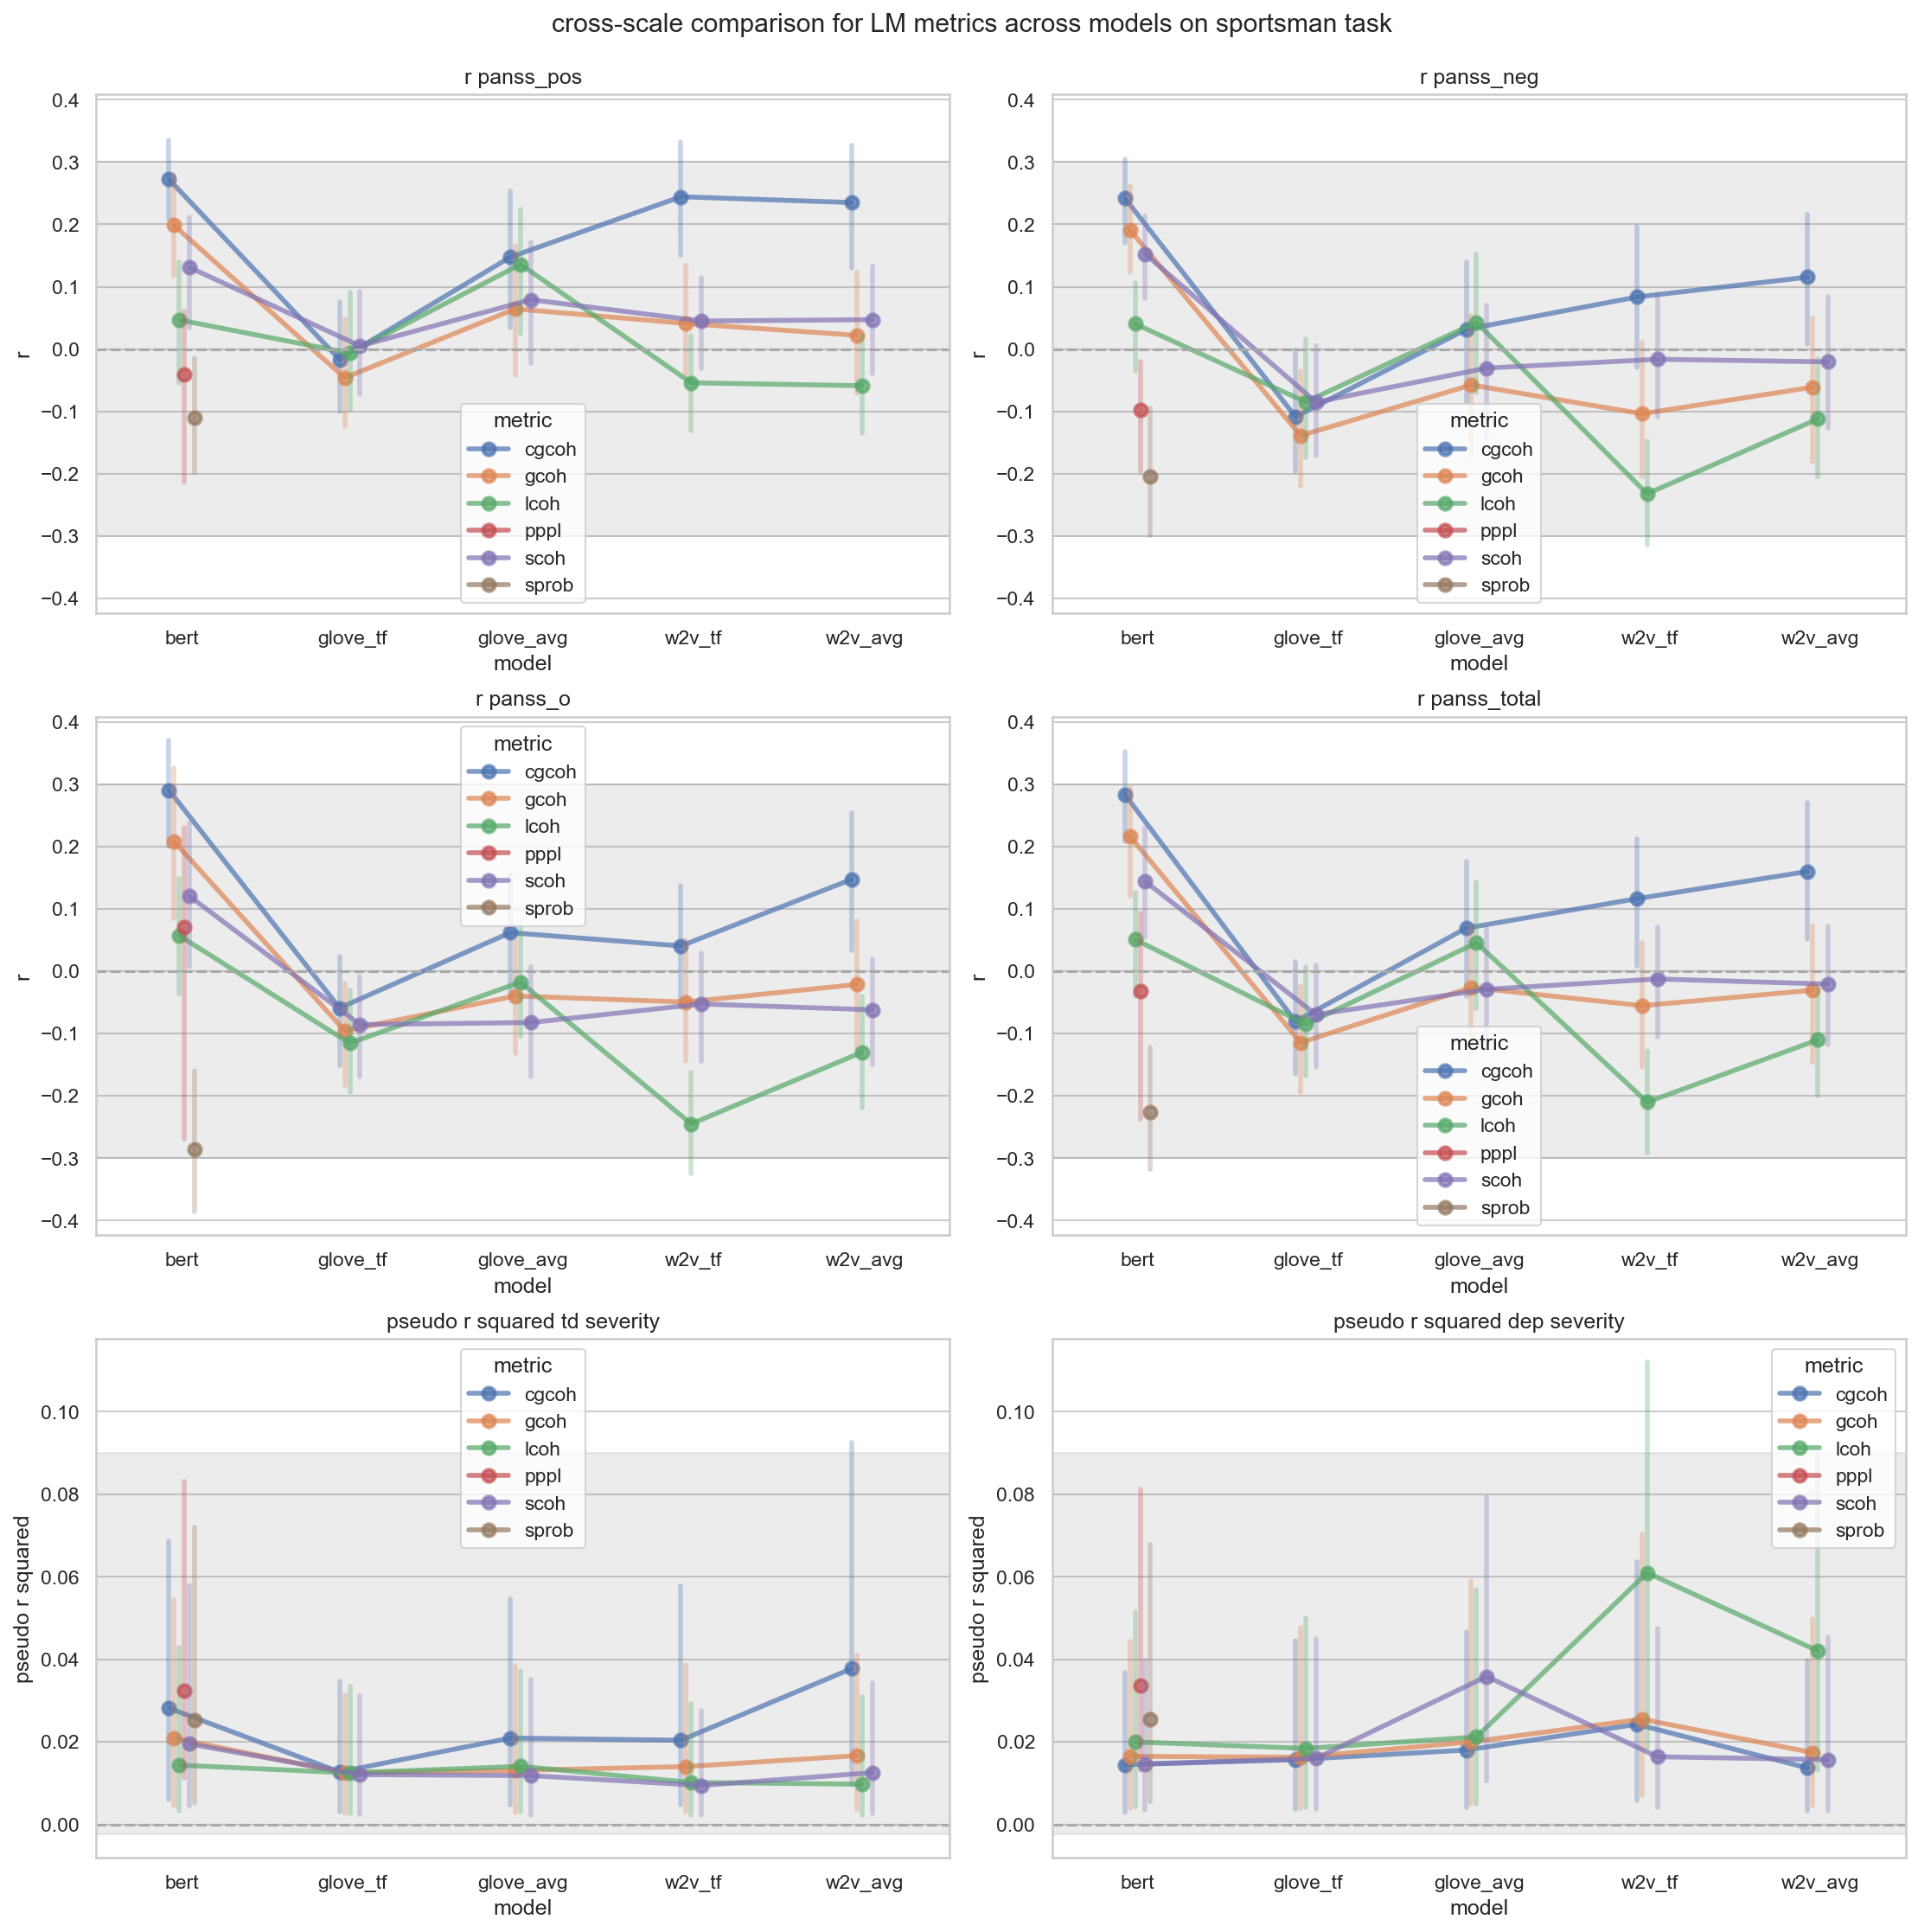
\includegraphics[width=1.1\textwidth, center]{Figures/chapter_4/LM/ru_sportsman_scale_r.png} 
% \captionsetup{width=\textwidth}
% \caption[LM Metrics: Russian, Sportsman Task]{\label{fig:results:lm:ru:sp} Pearson's r correlation coefficient and pseudo r squared for each scale for the language model-based metrics on the Russian dataset, sportsman task. Grey indicates the values below 0.3 threshold in absolute value or pseudo r squared below 0.09.}
% \end{figure}

% sportsman / BERT best model - best but also most difference between the metrics; BERT positive corr(except next sent pred); w2v tf idf no or negative corr; w2v average no corr or positive corr

\begin{figure}[ht!]
    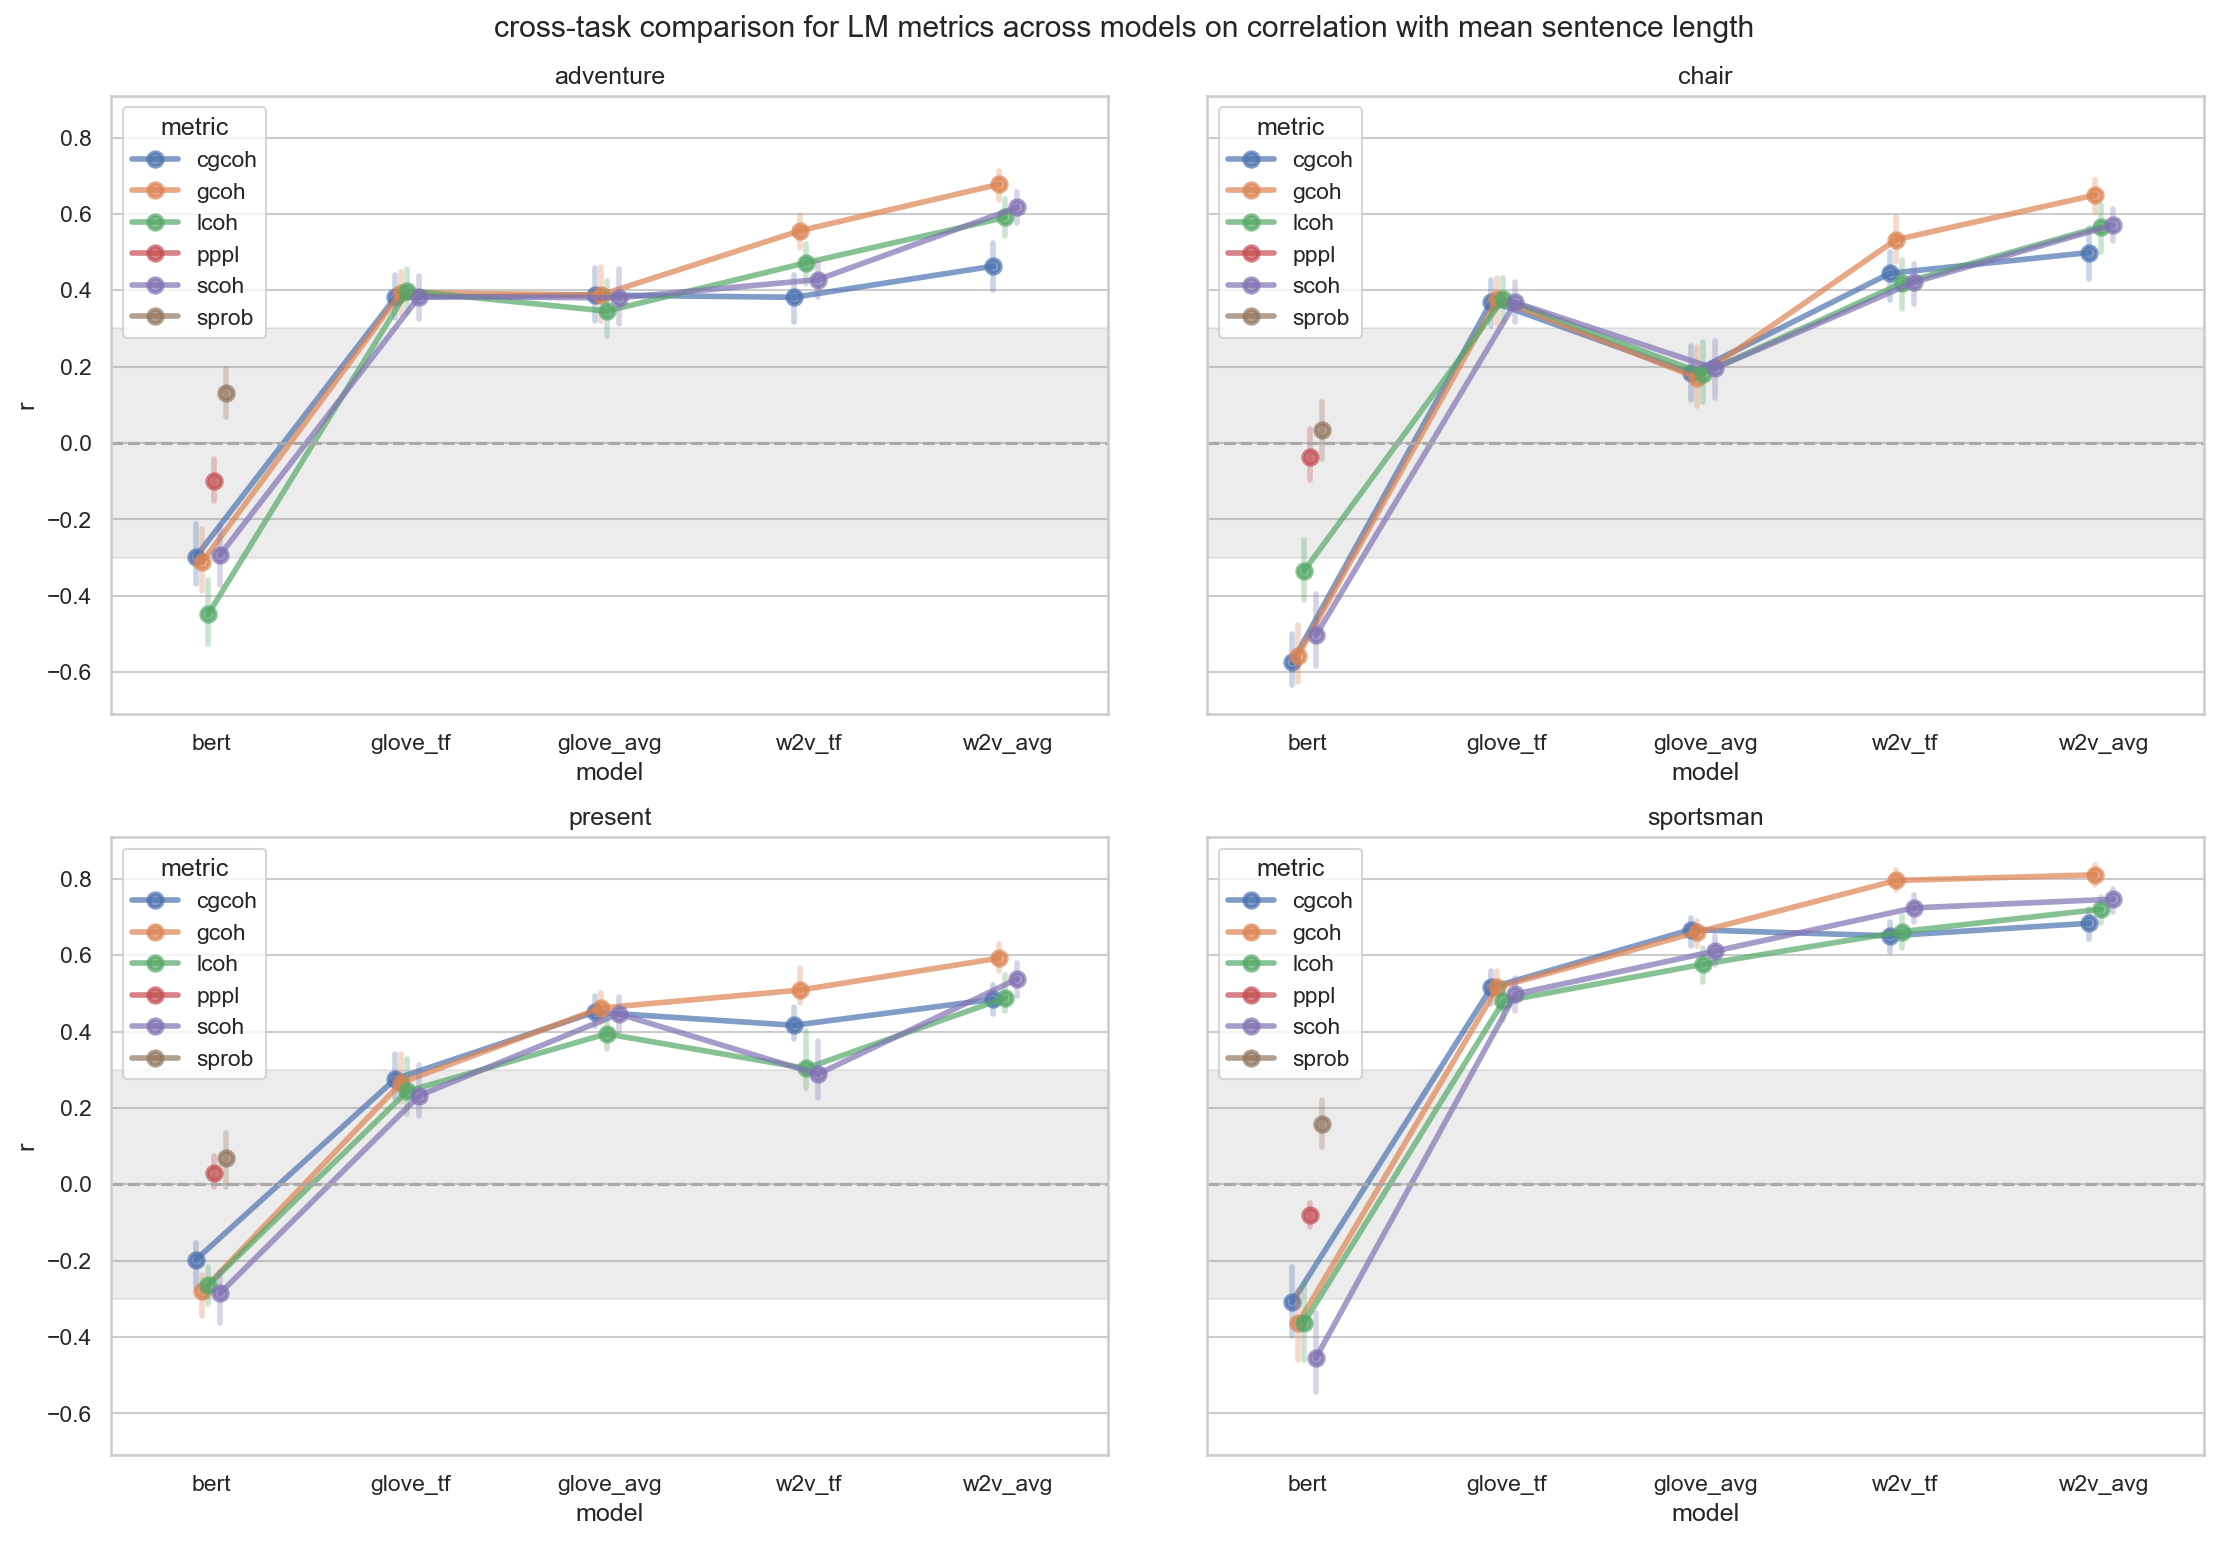
\includegraphics[width=1.1\textwidth, center]{Figures/chapter_4/LM/ru_corr_len.png} 
\captionsetup{width=\textwidth}
\caption[LM Metrics: Russian, Length Correlation]{\label{fig:results:lm:ru:corr_len} Pearson's r correlation coefficient with mean sentence length for the language model-based metrics on the Russian dataset across tasks. Grey indicates the values below 0.3.}
\end{figure}

Figure \ref{fig:results:lm:ru:corr_len} shows the strength of correlation with the mean sentence length across tasks, models, and metrics. 

% corr len
Cosine similarity-based metrics calculated using BERT, correlated negatively with mean sentence length, though the correlation was not equally strong across tasks and metrics, being above the threshold for all metrics on chair and sportsman tasks; only for local and global coherence on the adventure task; and for no metrics on present task. Next sentence probability and pseudo-perplexity did not correlate with length on any of the tasks. 
As for the metrics calculated using GloVe and word2vec, they correlated positively, rather than negatively, with mean sentence length. This correlation was stronger on averaged than on TF-IDF weighed embeddings for all tasks when word2vec was used, and for GloVe it was so on two tasks, sportsman and present, while on chair task the opposite was observed, and almost no difference was seen on the adventure task. All metrics calculated using word2vec correlated with mean sentence length on three tasks and on the fourth, present, second order coherence calculated using TF-IDF averaging did not exceed the threshold. The correlation was above the threshold for all GloVe metrics on sportsman and adventure tasks and was also so for TF-IDF GloVe on chair and for averaged GloVe on present tasks.

Interestingly, across all tasks, cosine similarity-based metrics calculated using BERT showed a positive correlation with the symptom scales and a negative correlation with mean sentence length, while the two non-contextualized embedding models tended to show a negative correlation with the symptoms scales and a positive one with the sentence length. 

There was no clear hierarchy between models or metrics across all tasks, as there was significant interaction between metrics and models, which was also different for different tasks. On average, perplexity, cumulative global coherence, and second-order coherence performed better in absolute correlation strength, while local and global coherence followed closely, and the next sentence probability tended to underperform. BERT and word2vec tended to outperform GloVe, and TF-IDF weighting tended to outperform simple averaging. The performance of word2vec and GloVe seems to be at least partially explained by correlation with mean sentence length.

Across the tasks, there was the same pattern, that cumulative global coherence tended to correlate more positively (or less negatively) than other metrics, and it was followed by global coherence, while local and second-order coherence tended to correlate more negatively. There was, however, a curious difference between the models, as cosine similarity-based metrics calculated using BERT tended also to correlate more positively (or less negatively) than either word2vec or GloVe, which both tended towards a negative correlation. These patterns, when combined, caused a significant model-metric interaction. 

% hierarchy of metrics
% sprob    0.123186
% gcoh     0.140981
% lcoh     0.146947
% scoh     0.153215
% cgcoh    0.153664
% pppl     0.166540

% hierarchy of models
% glove_avg    0.126972
% glove_tf     0.127707
% w2v_avg      0.148330
% w2v_tf       0.154666
% bert         0.180319

\subsection{Cross-Linguistic Comparison}

% German
% hierarchy of metrics (abs)
% cgcoh    0.120598
% gcoh     0.181313
% sprob    0.248705
% lcoh     0.295024
% scoh     0.311049
% pppl     0.340907

% corr len metrics (abs)
% cgcoh    0.284133
% gcoh     0.489777
% lcoh     0.549403
% scoh      0.55498
% sprob     0.57879
% pppl     0.536772

% hierarchy of models (abs)
% bert         0.176137
% glove_tf     0.193866
% glove_avg    0.212054
% w2v_avg      0.263709
% w2v_tf       0.289213

% corr len models (abs)
% bert         0.164279
% glove_tf     0.423349
% glove_avg    0.559389
% w2v_tf       0.588787
% w2v_avg      0.612061

% Russian
% hierarchy of metrics avg acorss tasks (abs)
% sprob    0.123186
% gcoh     0.140981
% lcoh     0.146947
% scoh     0.153215
% cgcoh    0.153664
% pppl     0.166540

% corr len metrics avg acorss tasks (abs)
% pppl     0.060895
% sprob    0.098309
% lcoh     0.431396
% cgcoh    0.431562
% scoh     0.449136
% gcoh     0.493385

% hierarchy of models  avg acorss tasks (abs)
% glove_avg    0.126972
% glove_tf     0.127707
% w2v_avg      0.148330
% w2v_tf       0.154666
% bert         0.180319

% corr len models avg acorss tasks (abs)
% bert         0.364786
% glove_tf     0.379823
% glove_avg    0.406061
% w2v_tf       0.500115
% w2v_avg      0.606063

% differences
There was, for LM-based metrics, little similarity between the languages or tasks. Interestingly, even the direction of correlation with symptoms differed between the samples, as BERT metrics tended to correlate positively with symptoms scales on the Russian sample, but negatively on the German one, where there was no difference in correlation direction between BERT and non-contextualized models. Similarly, pseudo-perplexity correlated positively with symptom severity on the German sample, but negatively on the Russian one, and the reverse was true for next sentence probability. Both these metrics correlated with mean sentence length on the German sample, not on the Russian one, where they were the least strongly correlated of all the metrics.

% similarity in direction of metric correlation pattern
There was a similarity in the tendency for more positive (or less negative) correlation for cumulative global and global coherence across the models and for more negative correlation with symptom severity for local and especially second-order coherence, which was present for both languages.

% corr len patterns
On the German sample, there was a much clearer hierarchy of models and metrics,  which was absent from the Russian sample across the tasks, as there were large differences in performance between them. On both samples, BERT correlated least with mean sentence length, though here, also, the direction of correlation differed between the samples, as on the Russian sample BERT-based metrics tended to correlate negatively with mean sentence length. On both samples TF-IDF clearly helped mitigate the correlation with length, yet, on the Russian sample, this pattern was somewhat weaker and task-dependent. Cumulative global coherence was clearly the least length-dependent for the German sample, but this pattern, if at all present, was also much weaker on the Russian sample. The relative performance of GloVe and word2vec, the latter outperforming the former, seems to be inversely related to the strength of their respective correlation with mean sentence length.

%-----------------------------------
%	section 8
%-----------------------------------
\clearpage
\section{Cross-Group Metric Comparison}
\label{sec:results:clinical:cross_group}

This section compares the performance of the metrics across metric types taking into account only the metrics that showed good performance, comprehending t-test error bars not intersecting zero, above threshold correlation with any of the scales, or above threshold predictive power. Additionally, metrics that were correlated with mean sentence length and performed worse than this baseline on all scales were excluded.

\subsection{German}

Figure \ref{fig:results:comp:de} compares the performance of the metrics across metric groups for all the psychiatric scales on the German sample. Among the metrics that performed well independently of sentence length, was BERT second-order coherence, which correlated negatively with the negative symptoms as well as general and total PANSS scores, and the same correlation pattern was also apparent for the rate of CCONJ. The only other length-independent metric was the AUX rate which correlated negatively with total SAPS score. 

Mean sentence length could only serve as a moderate baseline on the negative scales and PANSS total score. The rate of PART was correlated with length but consistently outperformed this baseline, and correlated positively with all the scales but PANSS positive. Four graph metrics, LCC, LSC, N, and E correlated with length but consistently outperformed it, negatively correlating with all but the two positive symptom scales. LTR showed weak positive correlation patterns, as it only outperformed mean sentence length on general PANSS, and for negative MALTR correlation, the only such scale was total SAPS score. 

\begin{figure}[ht!]
    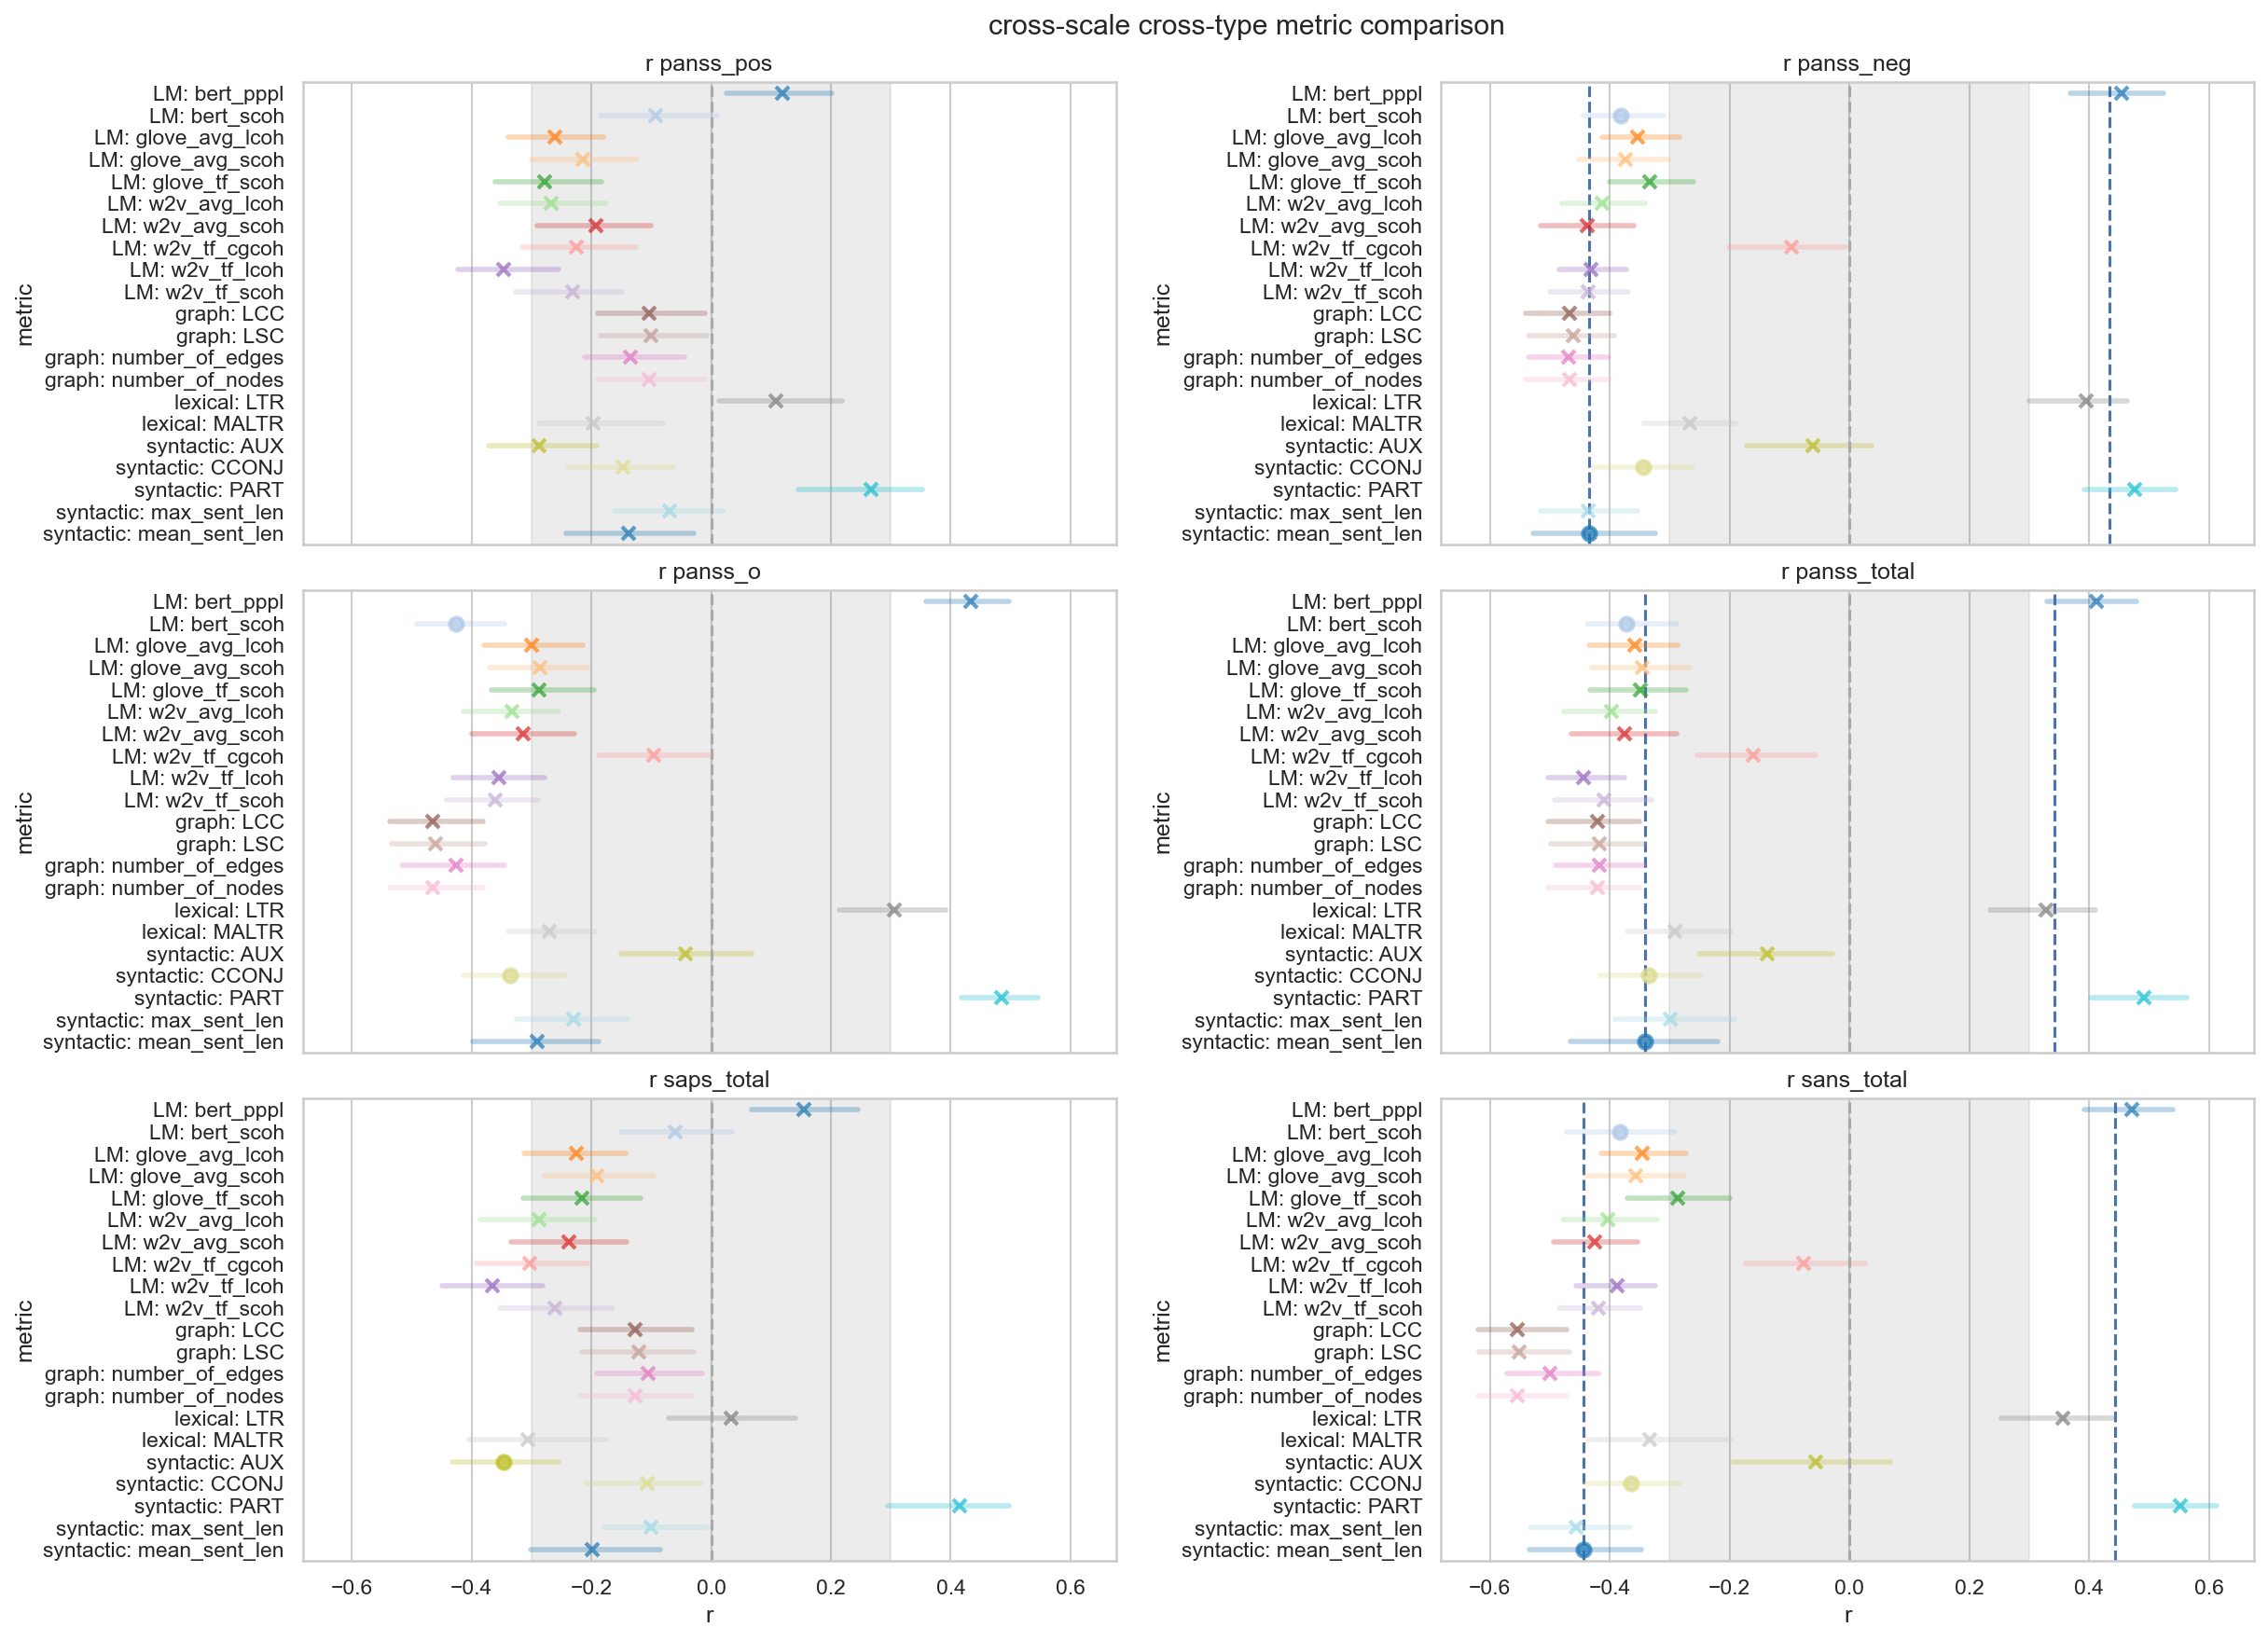
\includegraphics[width=1.1\textwidth, center]{Figures/chapter_4/compare/de_compare_r.png} 
\captionsetup{width=\textwidth}
\caption[Metric Comparison: German, Psychiatric Scales]{\label{fig:results:comp:de} Pearson's r correlation coefficient with each scale across well-performing metrics on the German dataset. Grey indicates the values below the 0.3 threshold in absolute value. The crossed dots indicate the metrics indicate either above-threshold correlation with mean sentence length or below-threshold correlation on a given scale. The mean sentence length baseline is shown by blue dashed line on the scales where this metric serves as a baseline. }
\end{figure}

BERT pseudo-perplexity score correlated more strongly than the mean sentence length baseline with negative and general symptom scales. BERT second-order coherence was uncorrelated with mean sentence length, and performed below the baseline on PANSS negative, but above it on SANS and PANS general and total scores. Averaged GloVe local coherence, which was correlated with length, barely correlated with general PANSS scale and was barely above mean sentence length in the negative correlation with PANSS total score. Averaged GloVe second-order coherence was similarly barely above mean sentence length on the negative correlation with PANSS total score. As for word2vec, all the metrics calculated using it correlated with mean sentence length, but frequently outperformed it, with TF-IDF weighted local coherence correlating with positive symptoms scales and outperforming length on the total PANSS score. Second-order coherence on TF-IDF weighted word2vec was weaker, outperforming the baseline only for PANSS general. Averaged local and second-order coherence calculated with word2vec were barely above the threshold and baseline for PANSS general and total. On the negative scales, where mean sentence length served as a reasonable baseline, all GloVe metrics were below it, while word2vec TF-IDF weighted and simply averaged second-order coherence barely outperformed the baseline for PANSS negative. Maximum sentence length barely outperformed mean sentence length on SANS total but on no other scale.

As negative symptoms predominated in the German sample, it was unsurprising that the performance was overall better on the negative and general symptom scales, with the only exception of the AUX rate. As could be expected, more pronounced patterns could be seen on SANS and SAPS than on the corresponding PANSS subscales. Overall, on the German sample, syntactic metrics showed the most promise, taking into account the mean sentence length baseline. Graph-based and lexical metrics seemed to be to some significant extent explaining the same effects as mean sentence length, yet outperformed this baseline in some cases. Finally, LM, except for pseudo-perplexity, was the least reliable group, with weak correlations, barely ever outperforming mean sentence length. 

\begin{figure}[ht!]
    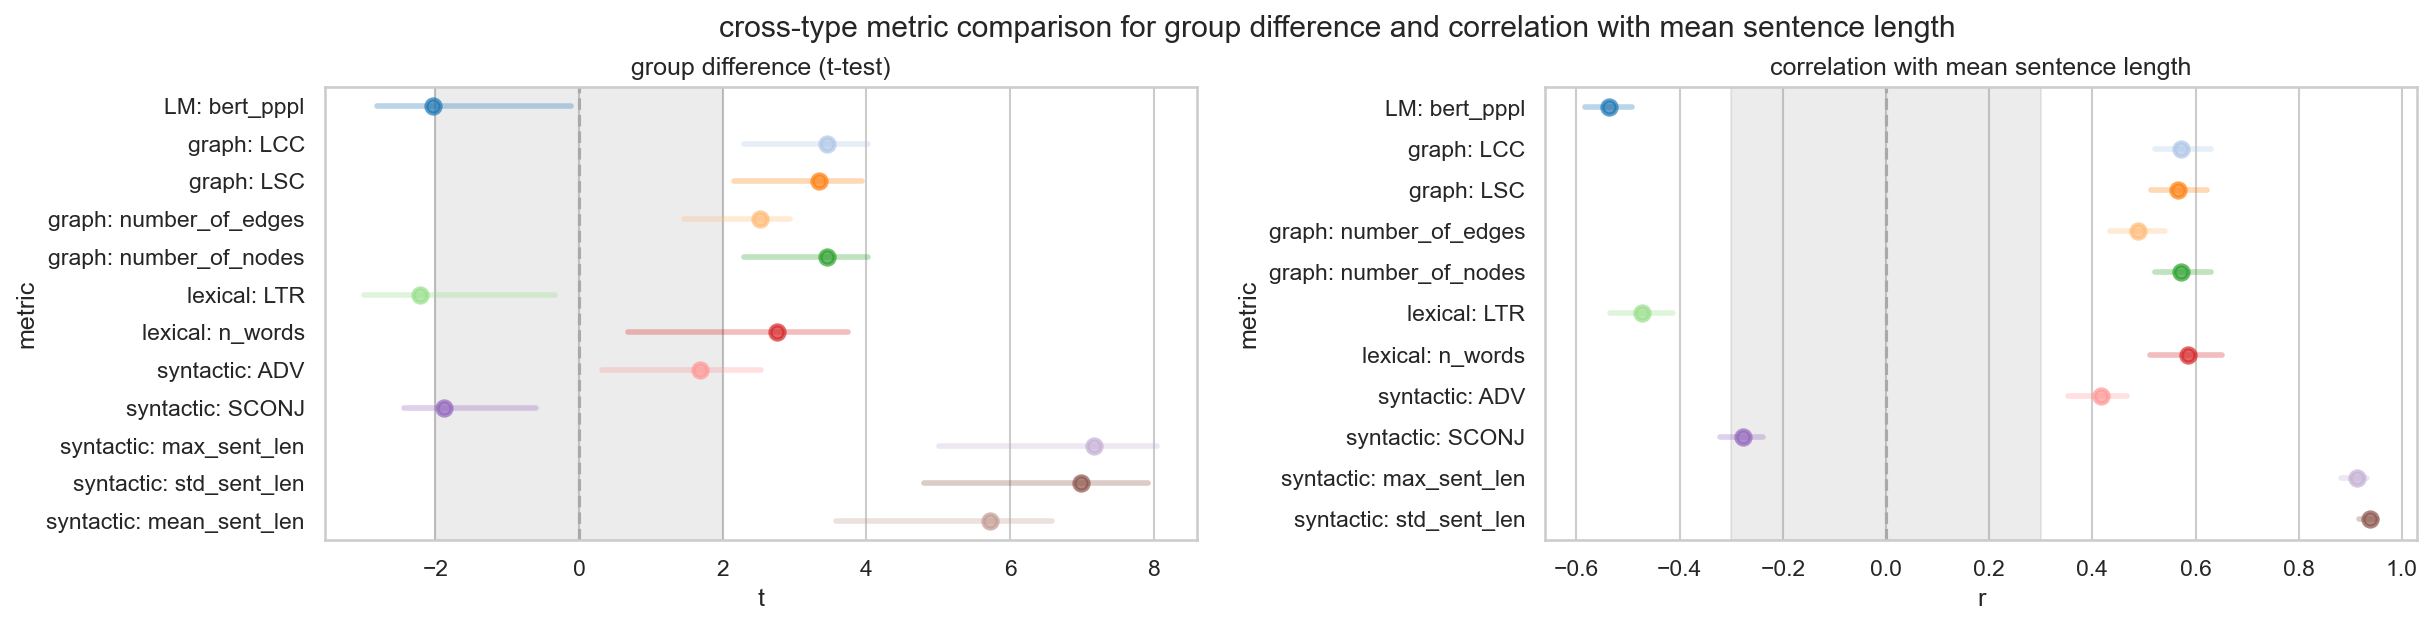
\includegraphics[width=1.1\textwidth, center]{Figures/chapter_4/compare/de_compare_t.png} 
\captionsetup{width=\textwidth}
\caption[Metric Comparison: German, T-Test]{\label{fig:results:comp:de:ttest} T-test and Pearson's r correlation coefficient with mean sentence length for the LM-based metrics on the German dataset. Grey indicates the values below 2 for t score and below the 0.3 threshold in absolute value for correlation coefficient. Only the metrics, for which error bars on T-test do not intersect zero, are shown.}
\end{figure}

Figure \ref{fig:results:comp:de:ttest} compares the t-test effect size to the correlation with mean sentence length for the metrics, the bootstrap 25/75 percentile error bars of which did not intersect zero on the t-test. For all the metrics, the t-test effect size corresponds quite closely with the strength and to the direction of the correlation with mean sentence length. The mean sentence length itself also served as a very strong baseline for the t-test, outperformed, but not significantly so, only by the maximum and standard deviation in mean sentence length. 

\subsection{Russian}

Figure \ref{fig:results:comp:ru} compares the performance of the metrics averaged across tasks for all the psychiatric scales on the Russian sample. The metrics that did not, on average, strongly correlated with length, and performed somewhat well were as follows. The number of words correlated negatively with all PANSS scales and was also predictive of TD severity. LTR, being inversely related to the word count, performed similarly but in the opposite direction, correlating positively with all PANSS scales, yet less strongly than the simple word count. The number of sentences on average correlated negatively with all PANSS scales but positive. Interestingly, the number of parallel edges was on average slightly above the baseline for the positive PANSS subscale.


\begin{figure}[ht!]
    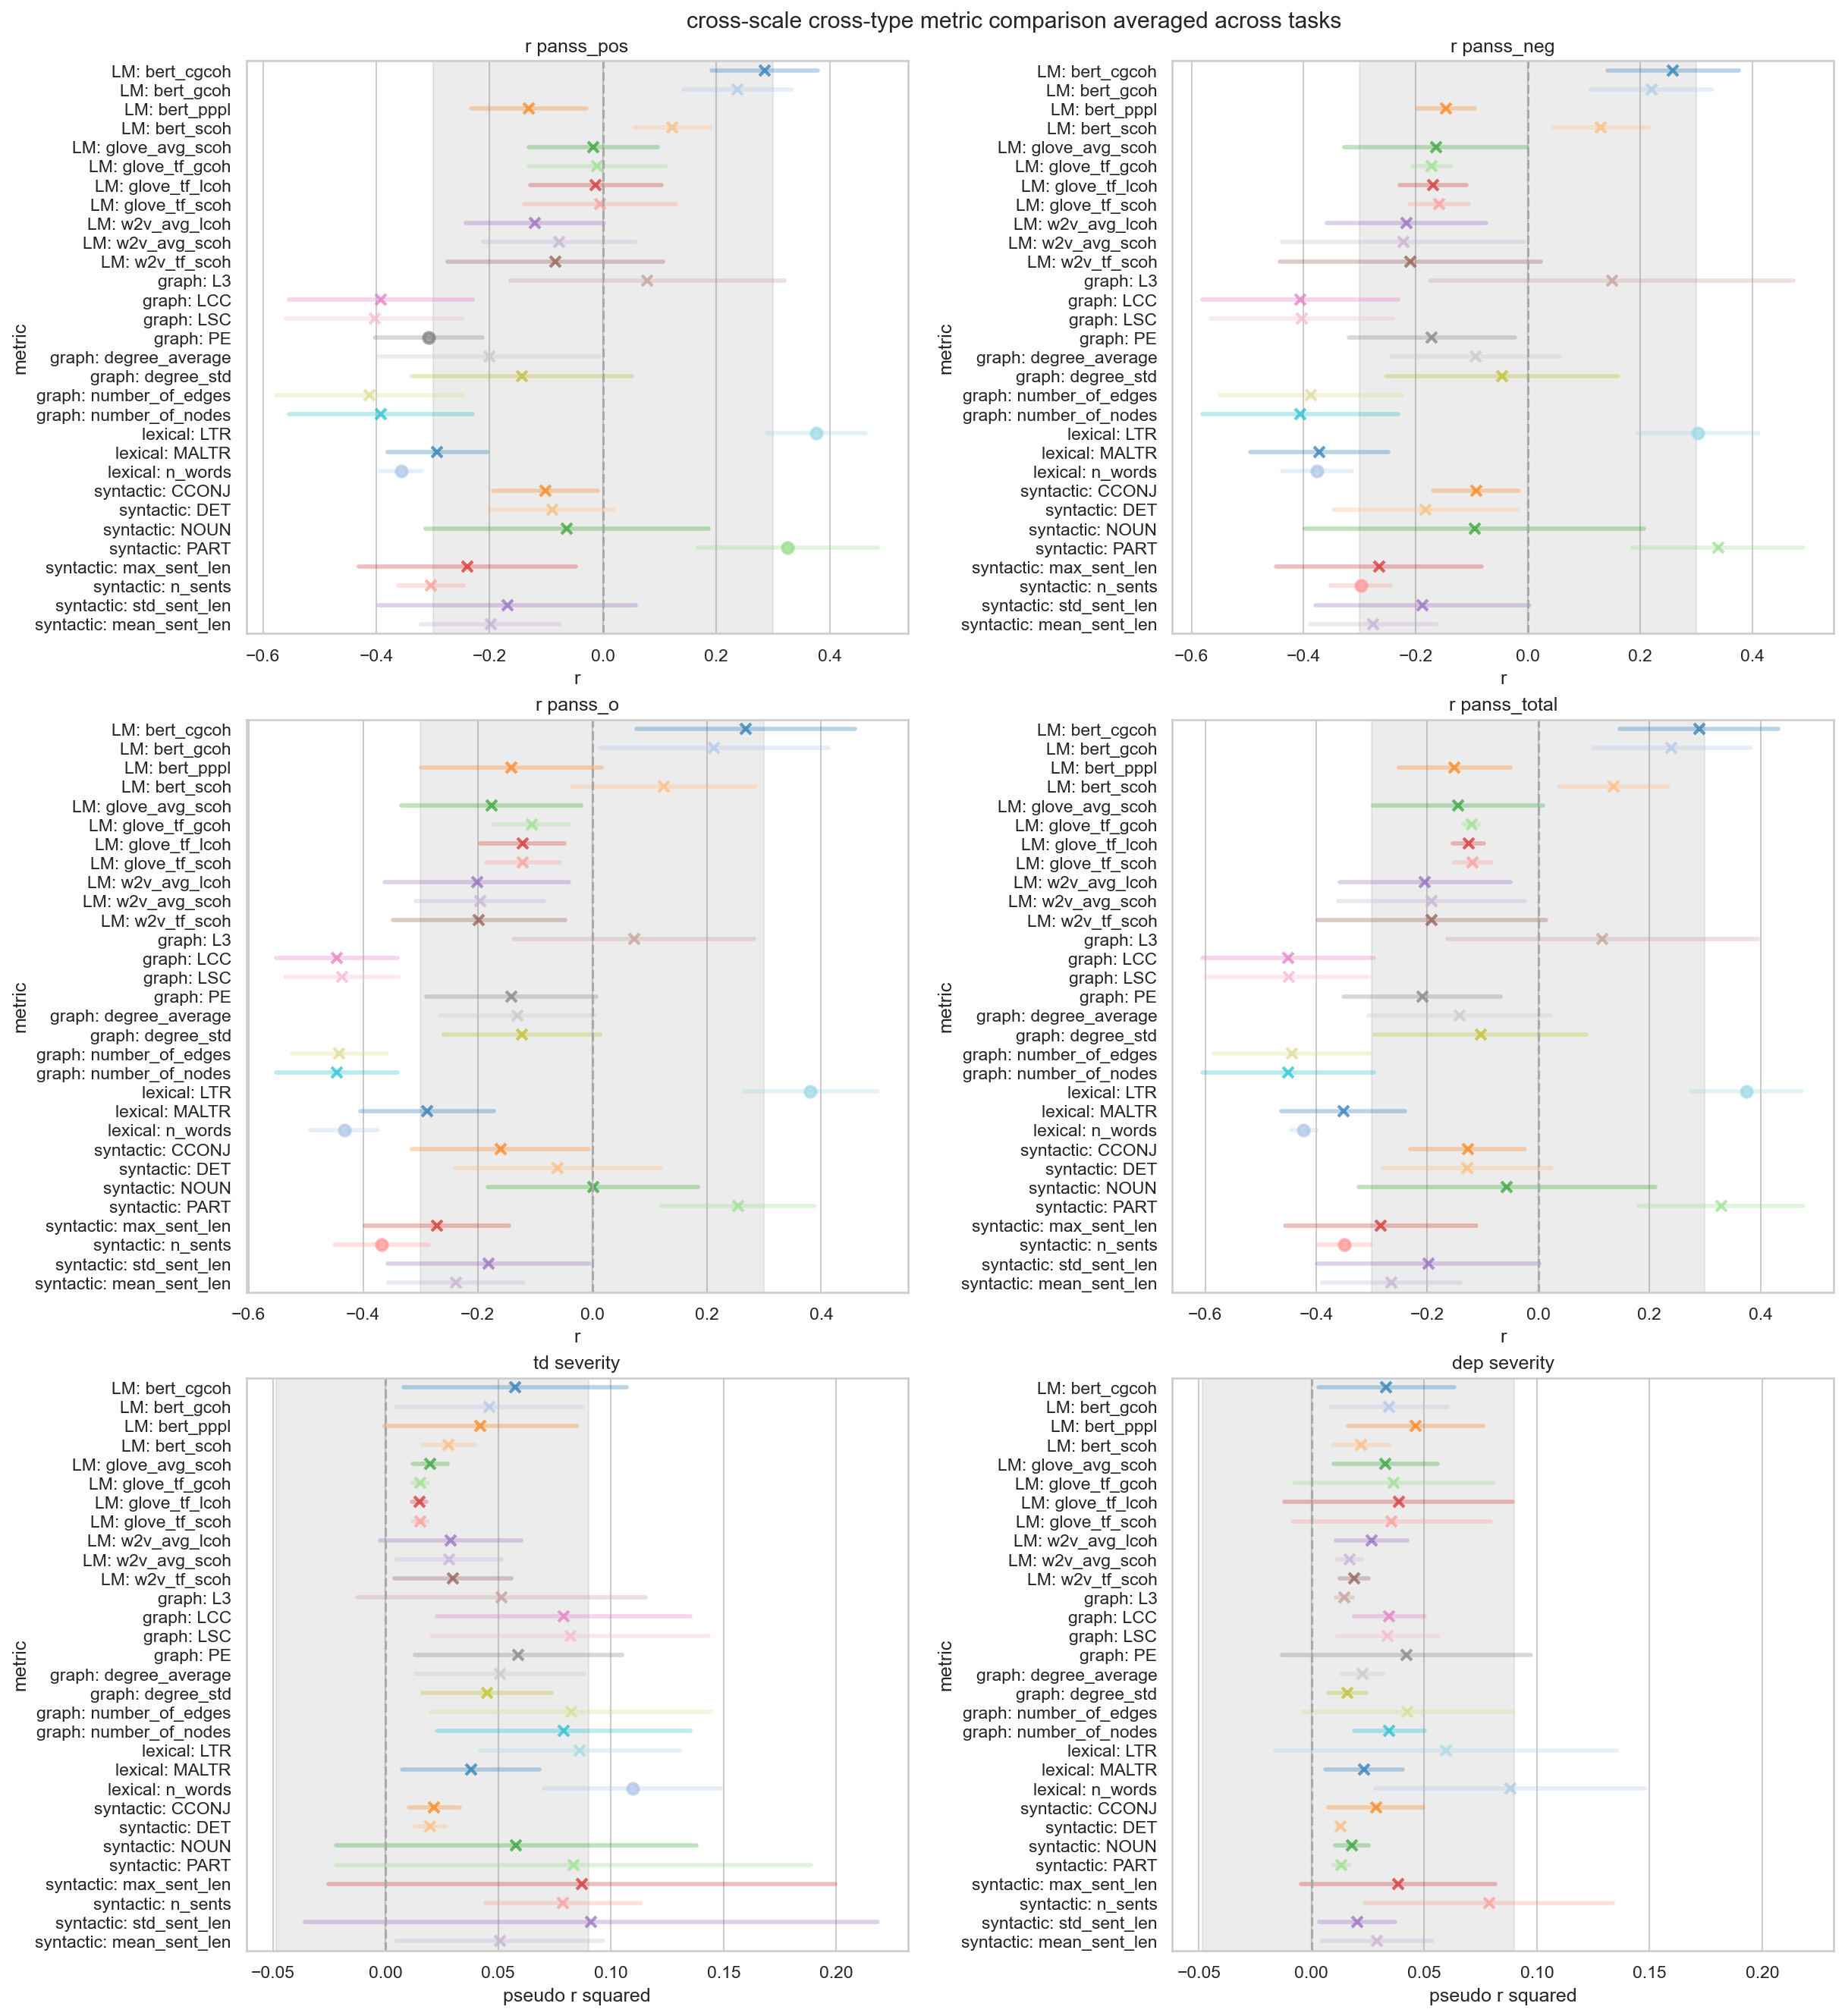
\includegraphics[width=1.1\textwidth, center]{Figures/chapter_4/compare/ru_cross_task_average_compare_r.png} 
\captionsetup{width=\textwidth}
\caption[Metric Comparison: Russian]{\label{fig:results:comp:ru}  Pearson's r correlation coefficient with each scale across well-performing metrics on the Russian dataset, averaged across tasks. Grey indicates the values below the 0.3 threshold in absolute value. The crossed dots indicate the metrics indicate either above-threshold correlation with mean sentence length or below-threshold correlation on a given scale. 
% The mean sentence length baseline is shown by blue dashed line on the scales where this metric serves as a baseline. 
Unlike other plots in this section, the error bars represent standard deviation, and the dot itself is the average value across the four tasks.}
\end{figure}

On the Russian sample, the mean sentence length did not, on average, serve as a reasonable baseline, because the differences were more pronounced in the number of sentences and words, rather than the length of sentences, as discussed above (\ref{sec:results:clinical:sample_length}). LCC, LSC, N, and E consistently outperformed this weak baseline and correlated negatively with all PANSS scales. The rate of PART correlated above baseline for all PANSS scales but the general. The standard deviation in mean sentence length was, on average, barely above the baseline in predicting TD severity. No LM metric was above baseline for any of the scales, when averaged across the four tasks. As depression severity could only be predicted on one task, no metric averaged across tasks, was predictive above baseline, with the number of words and sentences being the strongest predictors. No metric, even on the individual tasks, could differentiate between the groups reliably, as all error bars intersected zero.

\clearpage
Though there were some interactions between the scales and the metrics, the best-performing metrics showed similar results across scales, and the correlation direction was also the same.

On the Russian sample, verbosity was the most robust though not the strongest metric, but otherwise, the tested graph-based metrics outperformed the lexical and syntactic ones, and LM-based ones were by far the weakest.

\subsection{Cross-Linguistic Comparison}
\label{sec:results:clinical:cross_linguistic}

The difference between the languages was about as large as the difference between the tasks on the Russian sample, which, as the tasks were different between the languages, could be the main yet not the only cause for this difference. 

On both samples, LCC, LSC, N, and E were correlated with length, yet outperformed it in the strength of negative correlation with the psychiatric scales. PART rate, on the other hand, was also correlated with length and yet outperformed it in the strength of correlation, correlating positively with the psychiatric scales for both samples. LTR and MALTR correlated with length and were much weaker, sometimes performing worse than the mean sentence length baseline, especially on the German sample, where it was stronger. On the German sample mean sentence length was a stronger baseline than word count or sentence count, while the opposite was true on the Russian sample.

CCONJ rate performed well for the German sample, but weak on average, for the Russian sample. The mean sentence length, due to the differences covered in section \ref{sec:results:clinical:sample_length}, provided a moderate baseline for the German, but not the Russian sample. Instead, on the Russian sample the numbers of words and sentences were much stronger.

Among LM metrics, there was a surprising pattern, as the direction of correlation for BERT metrics was positive on the Russian sample but negative on the German one, and the direction of correlation was inverted for feature-based metrics as well as for cosine similarity-based ones. The perplexity performed well for the German, but not the Russian sample. Across both samples, cumulative global and global coherence correlated more positively with symptom severity than local and second-order coherence, which tended to correlate more negatively. Finally, there was a difference in the strength of correlation with mean sentence length between the languages. However, there was an overall pattern, more evident on the German sample, of BERT being least correlated with sentence length, followed by the TF-IDF and then by simply averaged non-contextualized models, and GloVe being less correlated than word2vec.

In both languages, relatively simple metrics, such as the word count, sentence count, or the number of nodes in the co-occurrence graph, i.e. moving window unique lemma count, showed the best performance, as compared to more complex metrics, such as LM-based ones. Co-occurrence graphs showed a promising result overall, and so did the syntactic metrics, though, the POS rates less so that simple unit length and count.